\section{Hardware Implementation}
\label{sec:hardware_impl}

% REORG_TAG: moved here from Kinematic Base Upgrade from Omnidirectional to Differential Drive
\subsection{Kinematic Base Redesign}

Extended operational testing of Tino's original omnidirectional Triskar base revealed systematic mechanical failures and control complexities that threatened system reliability during social interaction research. The three-wheel omnidirectional configuration, initially selected for maximum maneuverability, proved unsuitable for Tino's 20kg operational weight and predominantly forward-motion interaction patterns.

\subsubsection{System Failure Analysis and Design Requirements}

The original Triskar platform exhibited multiple failure modes under operational demands. Omniwheel rollers experienced systematic deformation, with surfaces becoming squared due to continuous plastic deformation under Tino's weight, creating irregular rolling characteristics that manifested as vibration, reduced traction, and unpredictable movement behavior. Roller bearing failures occurred frequently in the rear omniwheel due to dragging forces during movement operations, while the three-wheel configuration created uneven weight distribution with the rear wheel experiencing excessive drag forces that accelerated component wear.

\begin{figure}[H]
    \centering
    \includegraphics[width=0.5\textwidth]{Images/wire_triskar.png}
    \caption{Original Triskar Base System}
    \label{fig:original_Triskar_base}
\end{figure}

Motor performance analysis revealed inadequate torque delivery under sustained loading, with heating issues during extended use leading to performance degradation. The omnidirectional kinematics required sophisticated coordination between three drive motors while compensating for mechanical variability, creating control system complexity. Additionally, dependency on the VirHas library limited customization capabilities and created maintenance challenges for the Tino platform's specific requirements.

\subsubsection{Differential Drive Solution Design}

To address these limitations, a differential drive architecture was selected, prioritizing mechanical simplicity, enhanced reliability, and improved maintainability while providing adequate maneuverability for Tino's social interaction requirements. The design eliminates omnidirectional complexity while maintaining essential mobility through a two-wheel configuration with rear caster support that provides stable platform dynamics with reduced component count.

\begin{figure}[H]
    \centering
    \includegraphics[width=0.7\textwidth]{Images/NewBaseDifferentialDrive.jpg}
    \caption{Complete Differential Drive Base with T-Structure Framework}
    \label{fig:differential_base_complete}
\end{figure}

Weight distribution optimization utilizes the two front drive wheels to support the majority of Tino's operational weight while the rear caster provides stability without bearing significant driving loads, eliminating the dragging forces that compromised the original system. Maneuverability analysis demonstrates that differential drive provides adequate turning capability through differential wheel speed control, with simplified kinematics enabling more precise movement control and improved repeatability. This architecture proved highly effective, providing the reliable mobility foundation necessary for supporting the enhanced computational requirements of the power system upgrade detailed in the following section.

\subsubsection{Mechanical Implementation and System Integration}

The mechanical implementation required comprehensive base reconstruction utilizing aluminum Item profiles to create a robust T-structure framework. This modular profile system provides structural rigidity while enabling mechanical adjustments without complete system redesign, with wheel spacing optimization through the adjustable T-structure enabling fine-tuning of track width to achieve proper balance and stability characteristics.

\begin{figure}[H]
    \centering
    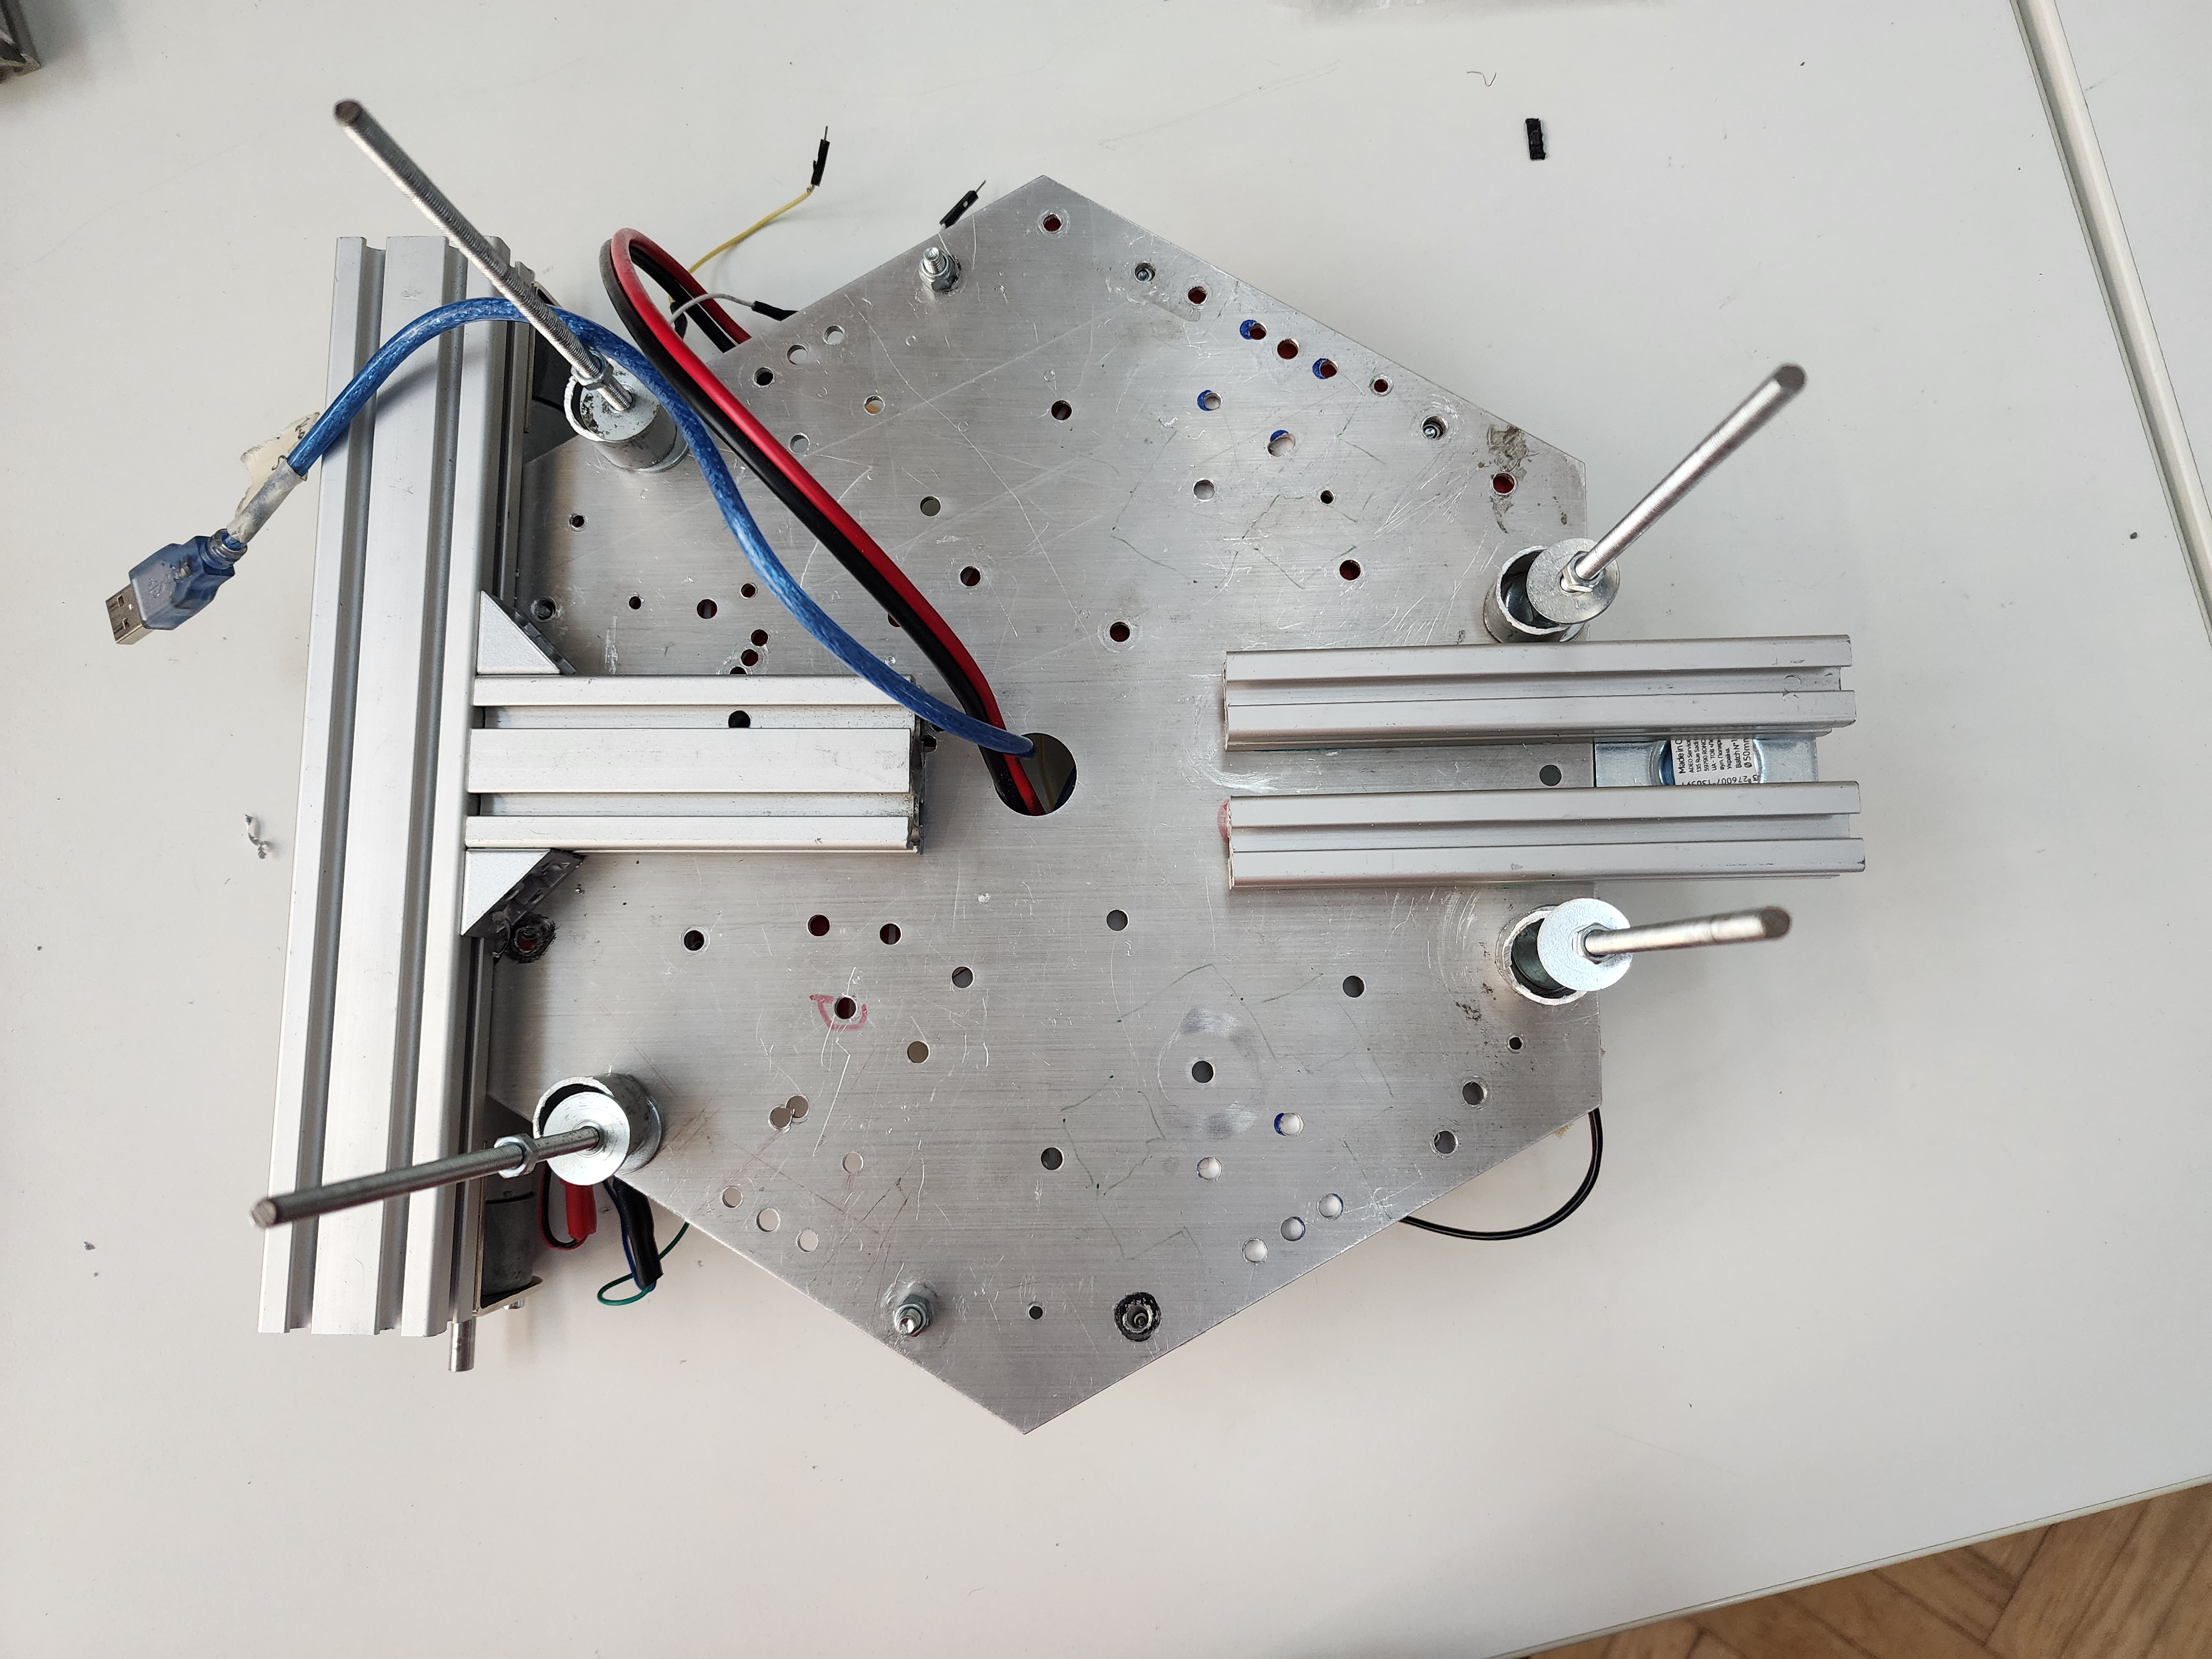
\includegraphics[width=0.6\textwidth]{Images/NewBaseDifferentialDrive (5).jpg}
    \caption{Top View of Differential Drive Base with T-Structure}
    \label{fig:differential_base_top}
\end{figure}

Motor mounting points integrate directly with the Item profile system through custom brackets providing precise alignment and secure attachment. The motor upgrade to more powerful units addresses the thermal and torque limitations of the original system, with new motors providing enhanced heat dissipation capabilities and higher continuous torque ratings suitable for Tino's operational requirements. Motor driver upgrade to the MDD10A units provides increased current handling capability and enhanced control responsiveness compared to the original dual-driver configuration.

\begin{figure}[H]
    \centering
    \begin{minipage}{0.45\textwidth}
        \centering
        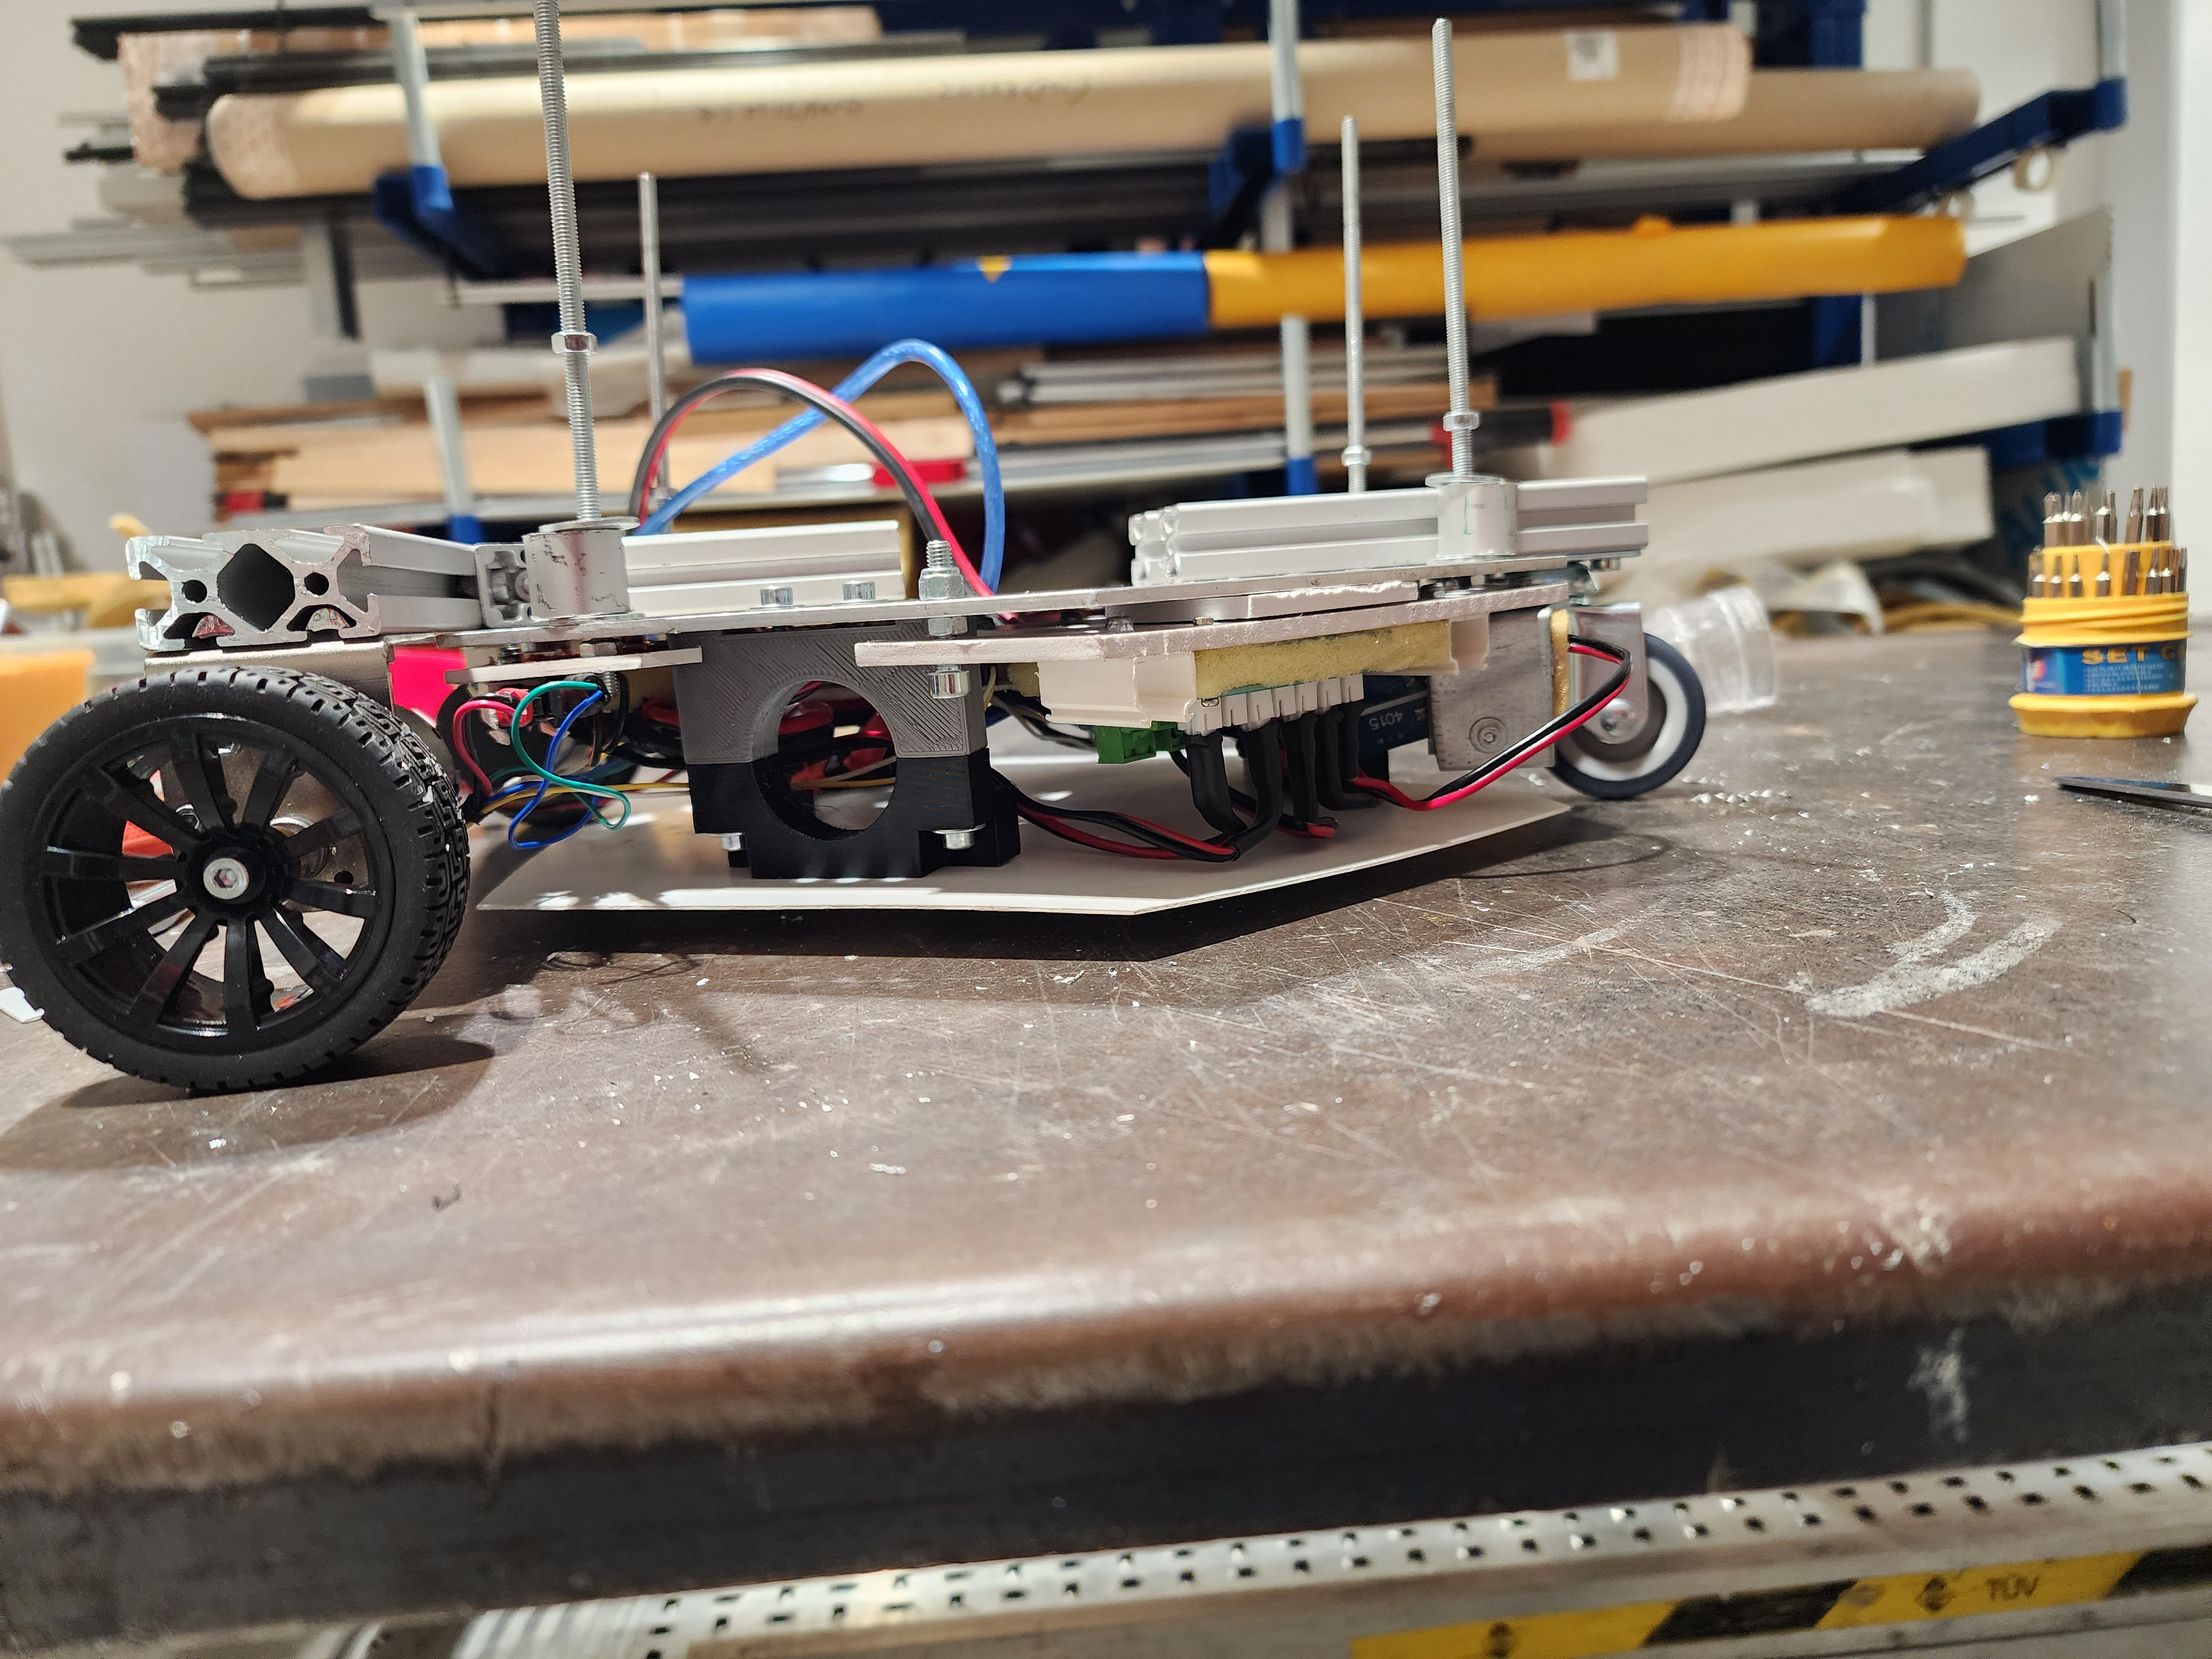
\includegraphics[width=\textwidth]{Images/NewBaseDifferentialDrive (2).jpg}
        \caption{Differential Drive Base Side View}
        \label{fig:differential_base_side}
    \end{minipage}
    \hfill
    \begin{minipage}{0.45\textwidth}
        \centering
        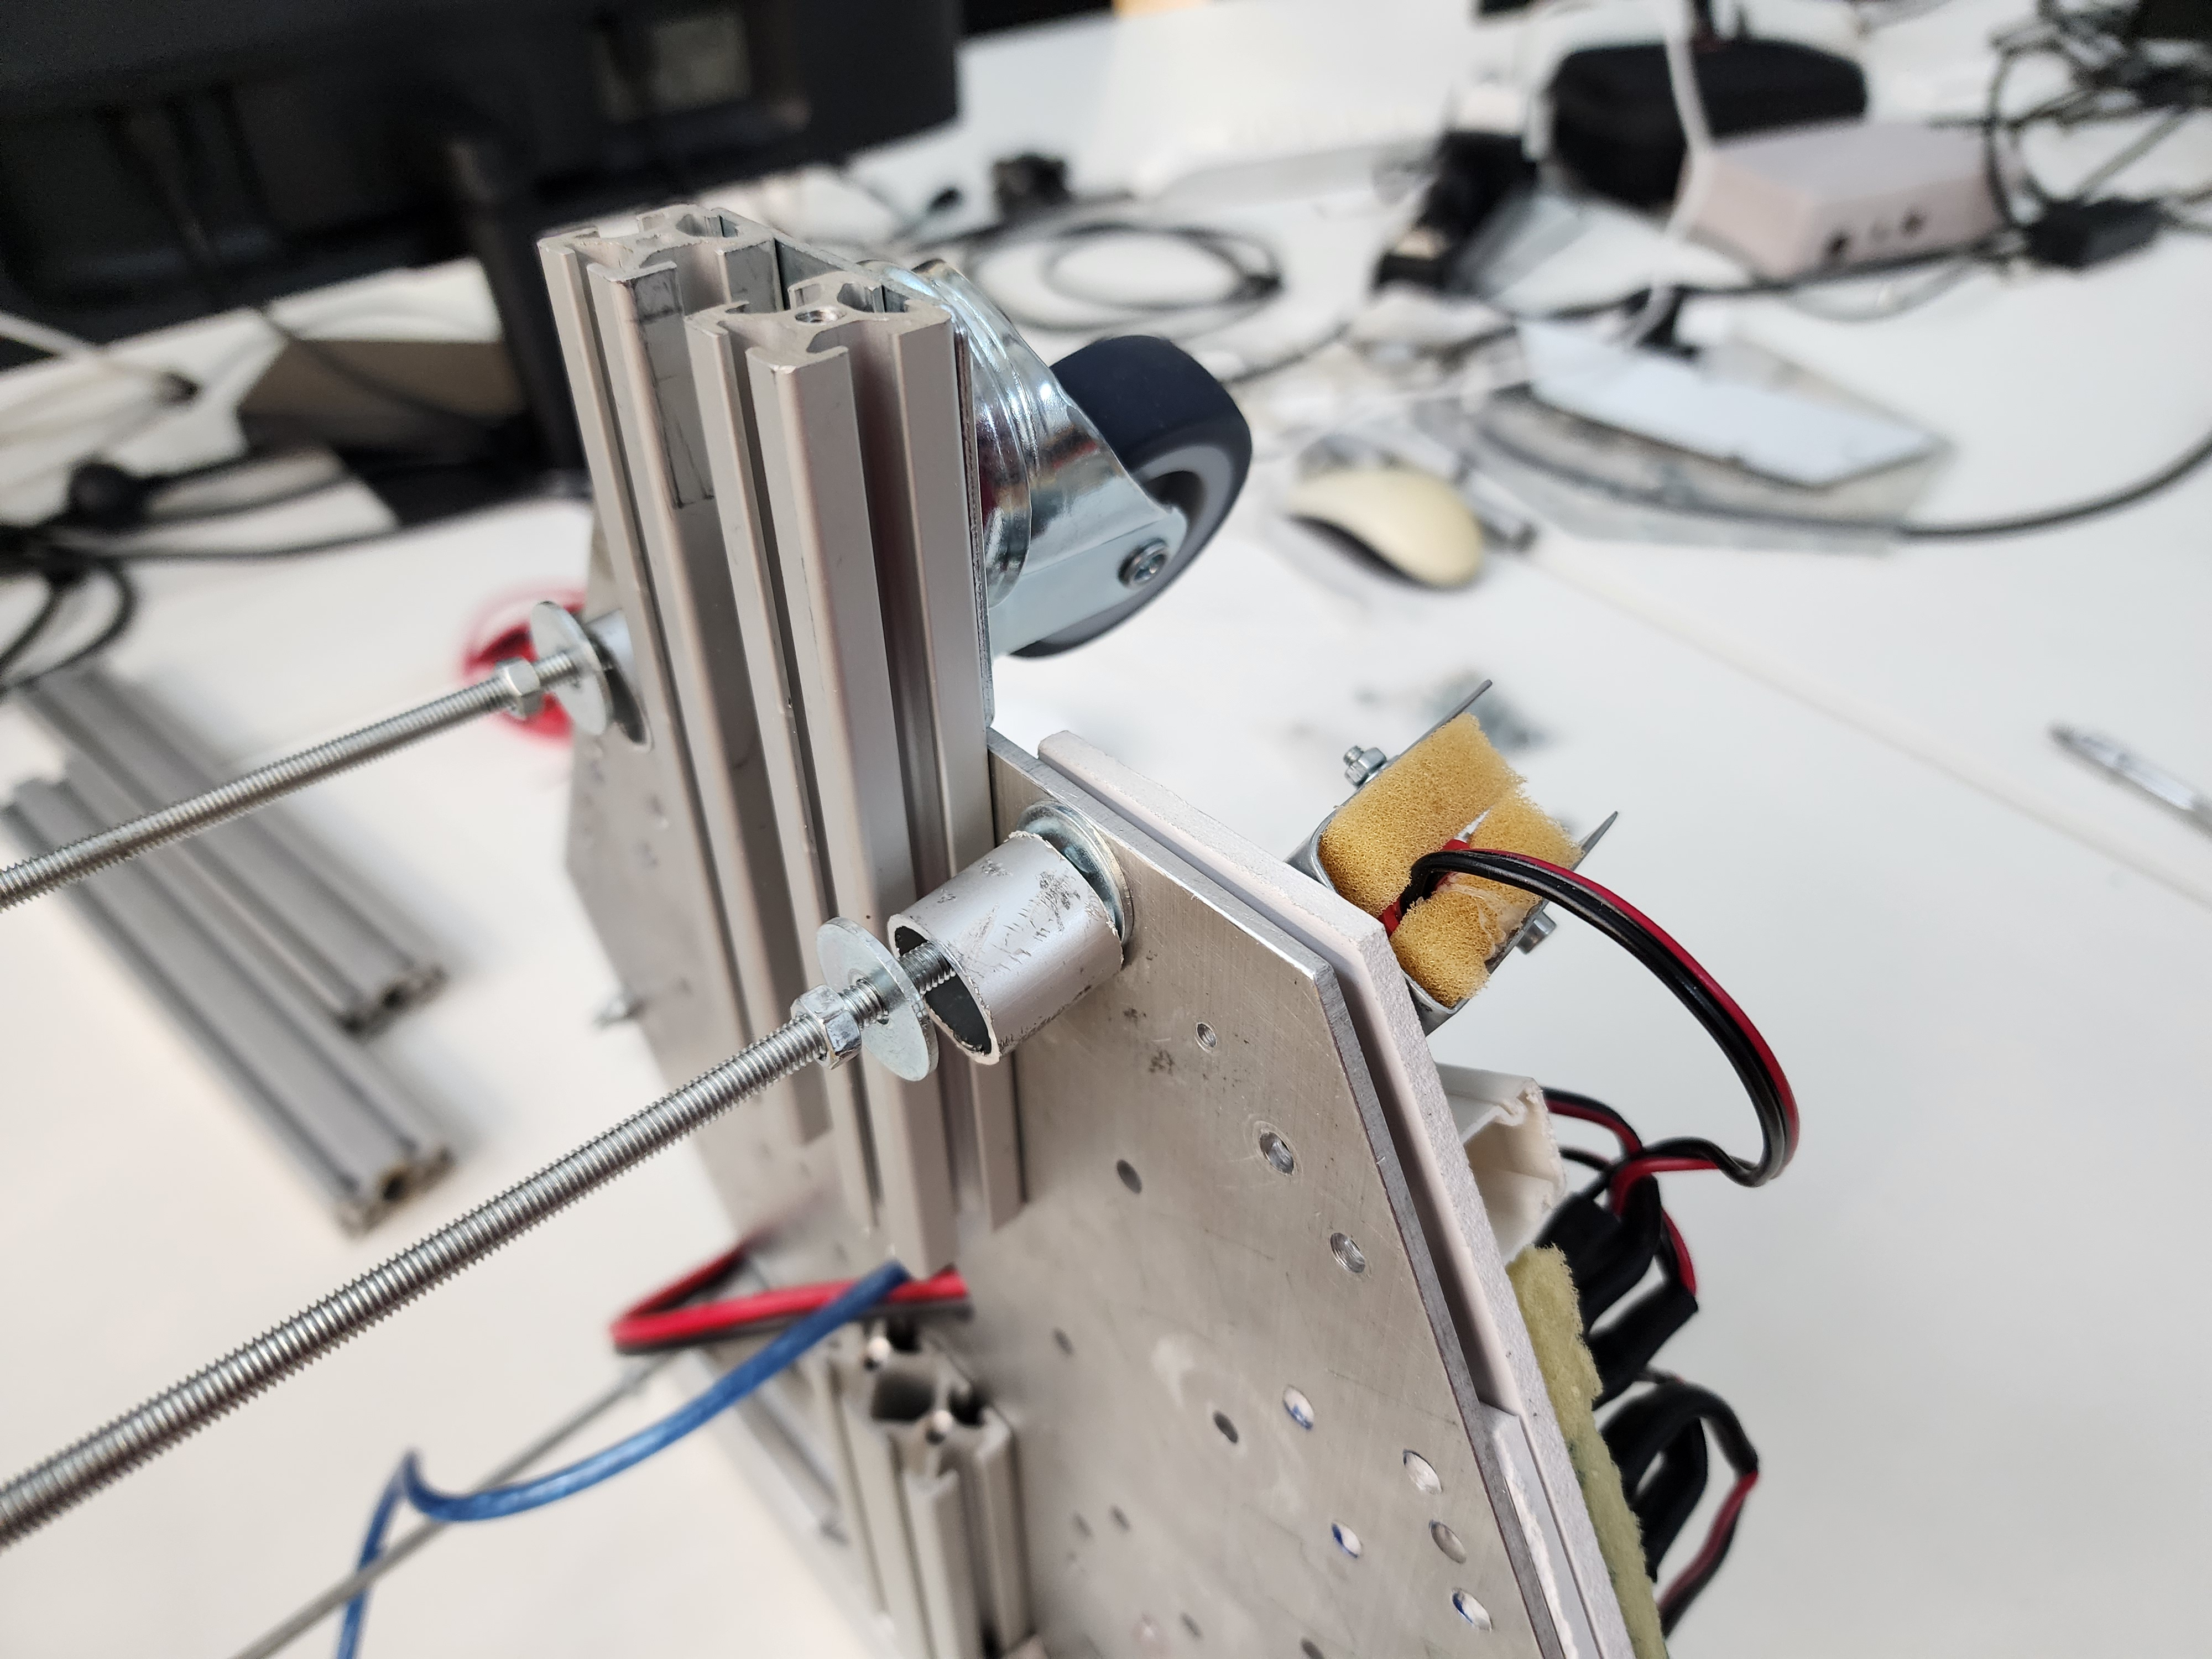
\includegraphics[width=\textwidth]{Images/NewBaseDifferentialDrive (3).jpg}
        \caption{Caster Wheel supporting Rear of Base}
        \label{fig:differential_base_caster}
    \end{minipage}
\end{figure}

\begin{figure}[H]
    \centering
    \begin{minipage}{0.45\textwidth}
        \centering
        \includegraphics[width=\textwidth,angle=-90]{Images/BaseNewMotors.jpg}
        \caption{Base with New Motors (Top View)}
        \label{fig:base_new_motors}
    \end{minipage}
    \hfill
    \begin{minipage}{0.45\textwidth}
        \centering
        \includegraphics[width=\textwidth,angle=-90]{Images/BaseNewMotors2.jpg}
        \caption{Base with New Motors (Close up Side View)}
        \label{fig:base_new_motors_side}
    \end{minipage}
\end{figure}

\subsubsection{Wheel System and Control Integration}

The wheel selection process revealed challenges with plastic hub construction under operational loads, requiring iterative development to achieve reliable traction and durability. Initial plastic wheels with pneumatic rubber tires provided adequate traction but suffered from hub failure and tire debeading issues when rubber separated from plastic hubs due to inadequate bonding strength. The solution involved wheel hub reinforcement through hot-glue filling, which addressed structural weakness while maintaining traction characteristics, though representing a temporary fix requiring future system upgrade.

\begin{figure}[H]
    \centering
    \begin{subfigure}{0.45\textwidth}
        \centering
        \includegraphics[width=\textwidth]{Images/WheelSilicona (3).jpg}
        \caption{Wheel Front View}
        \label{fig:wheel_hotglue}
    \end{subfigure}
    \hfill
    \begin{subfigure}{0.45\textwidth}
        \centering
        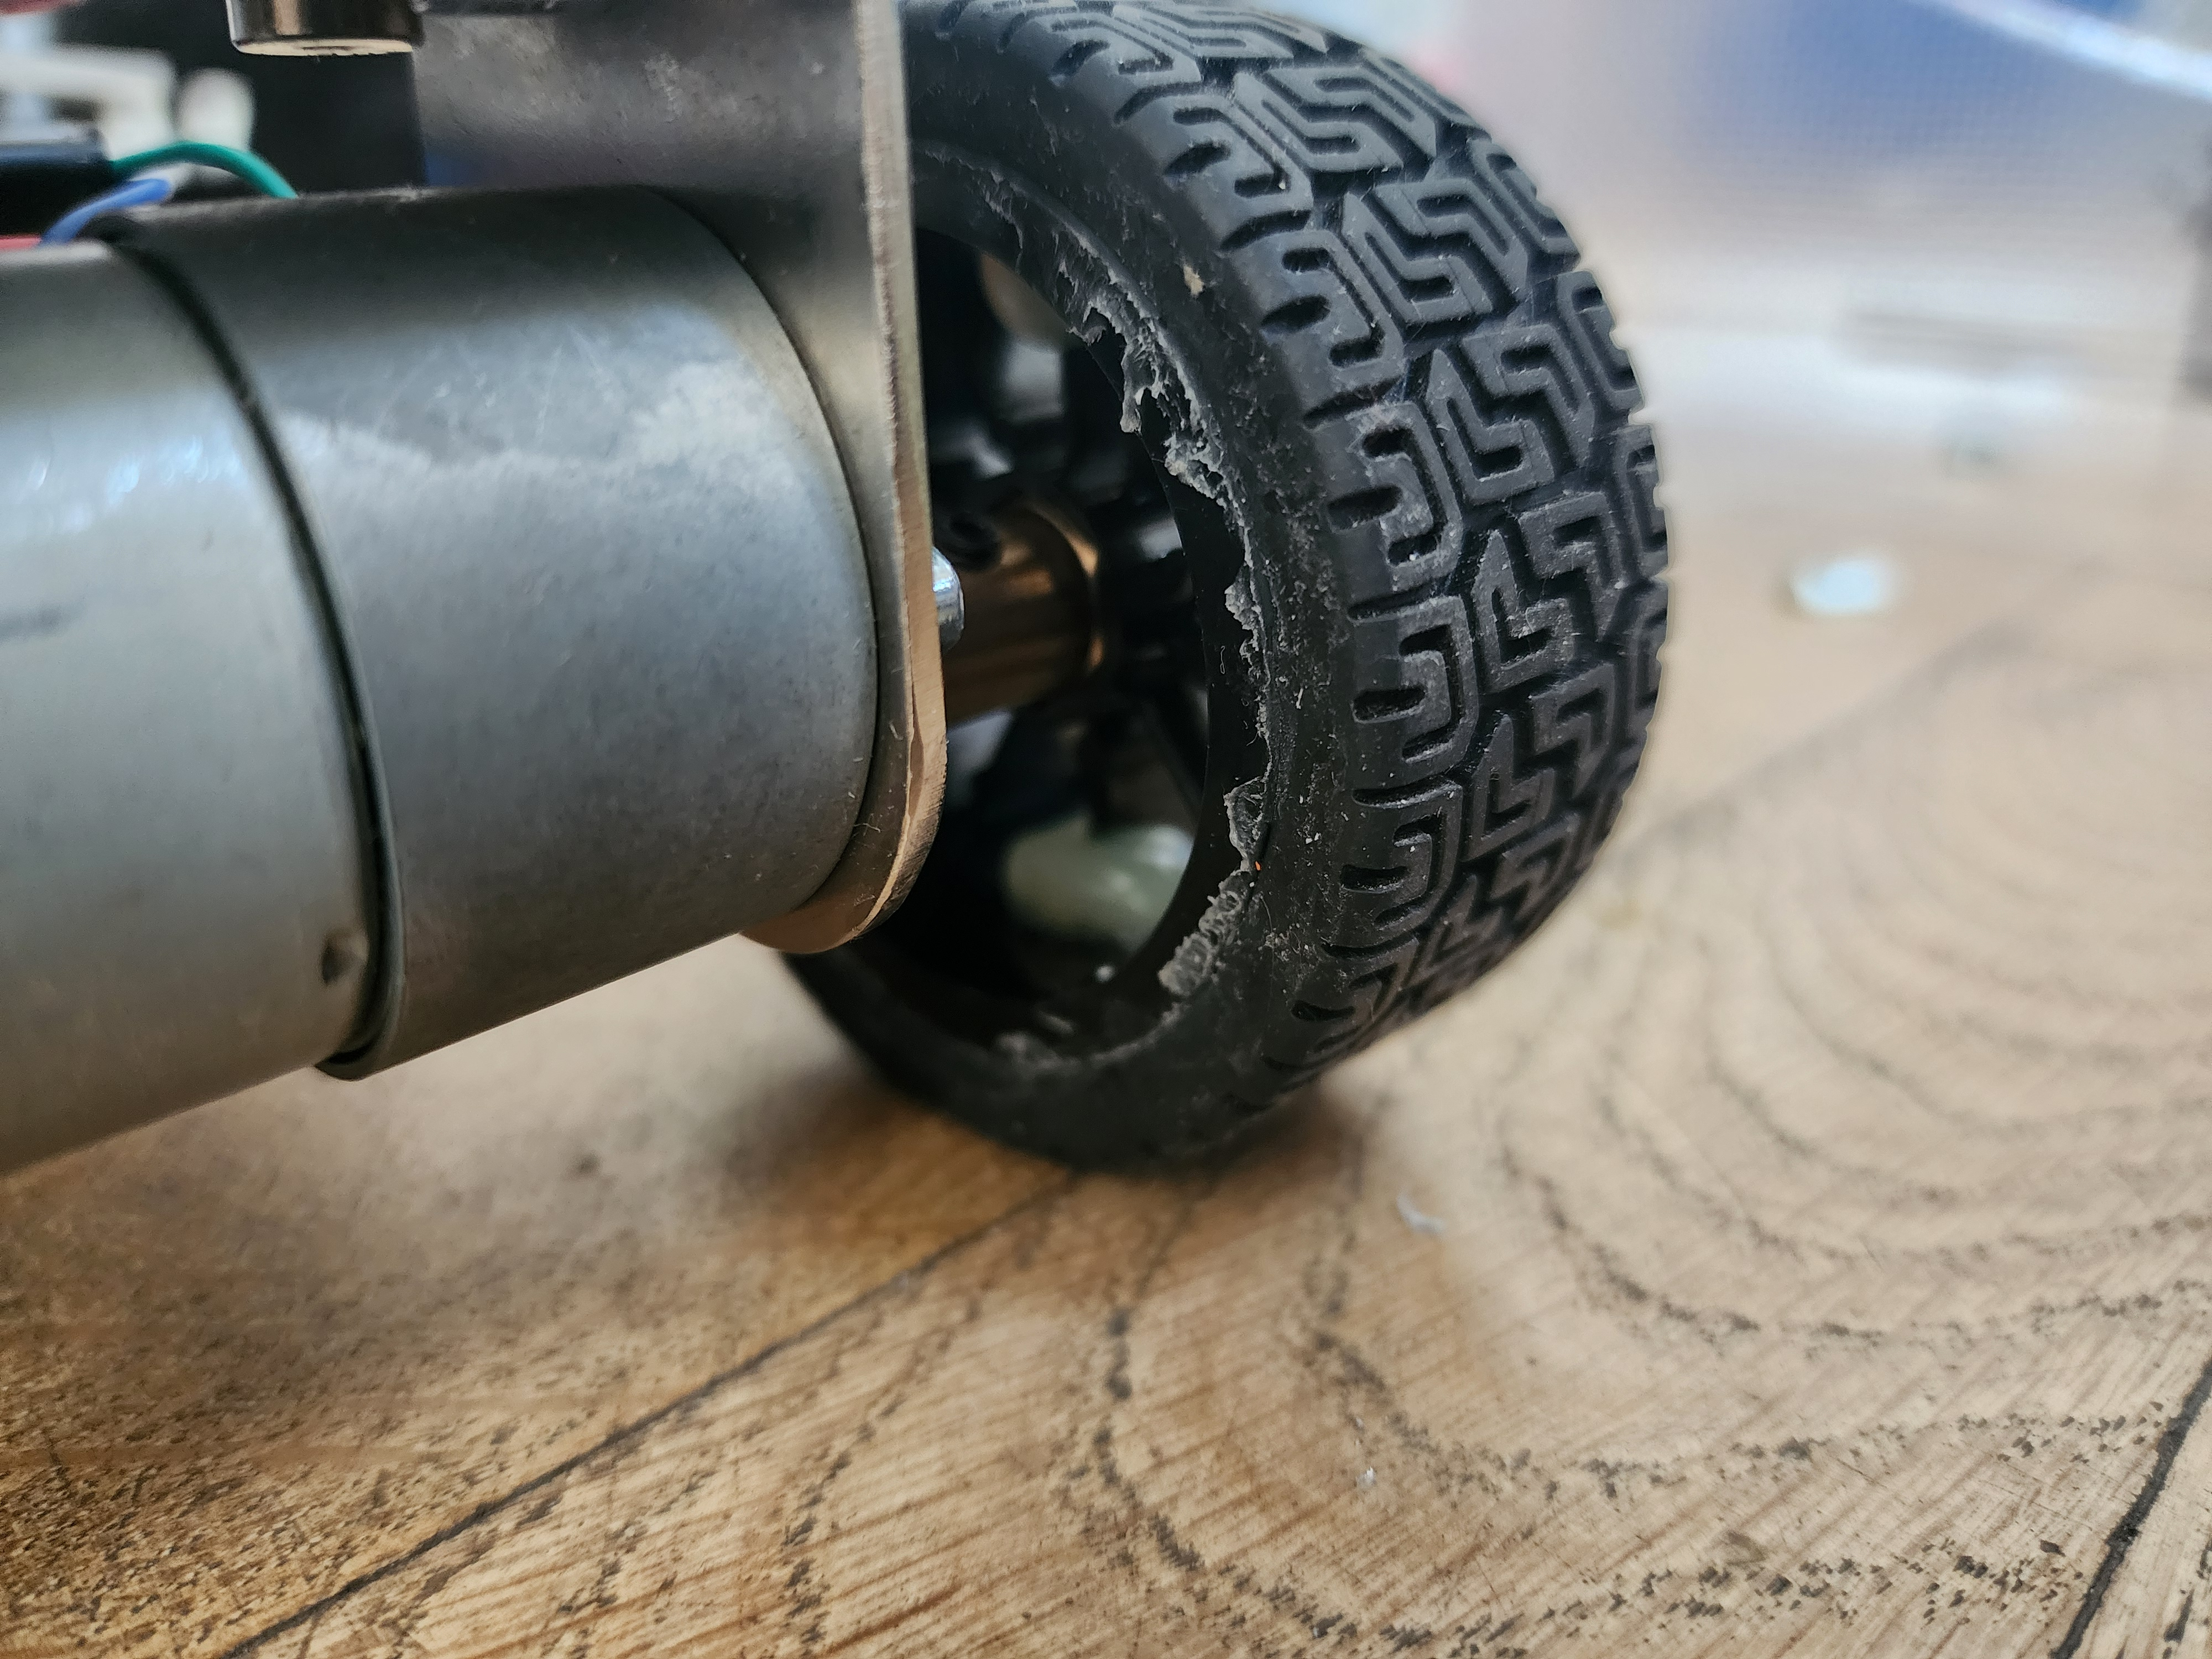
\includegraphics[width=\textwidth]{Images/WheelSilicona.jpg}
        \caption{Wheel Mounted on Motor Shaft}
        \label{fig:wheel_silicone}
    \end{subfigure}
    \caption{Wheel with Hot-Glue Filled Tires}
    \label{fig:combined}
\end{figure}

Fabric interference prevention required protective bumper implementation to prevent Tino's fabric covering from interfering with wheel operation. The bumper design provides physical separation between moving wheels and flexible fabric structure, with effectiveness testing demonstrating successful prevention of fabric entanglement in most operational scenarios.

\begin{figure}[H]
    \centering
    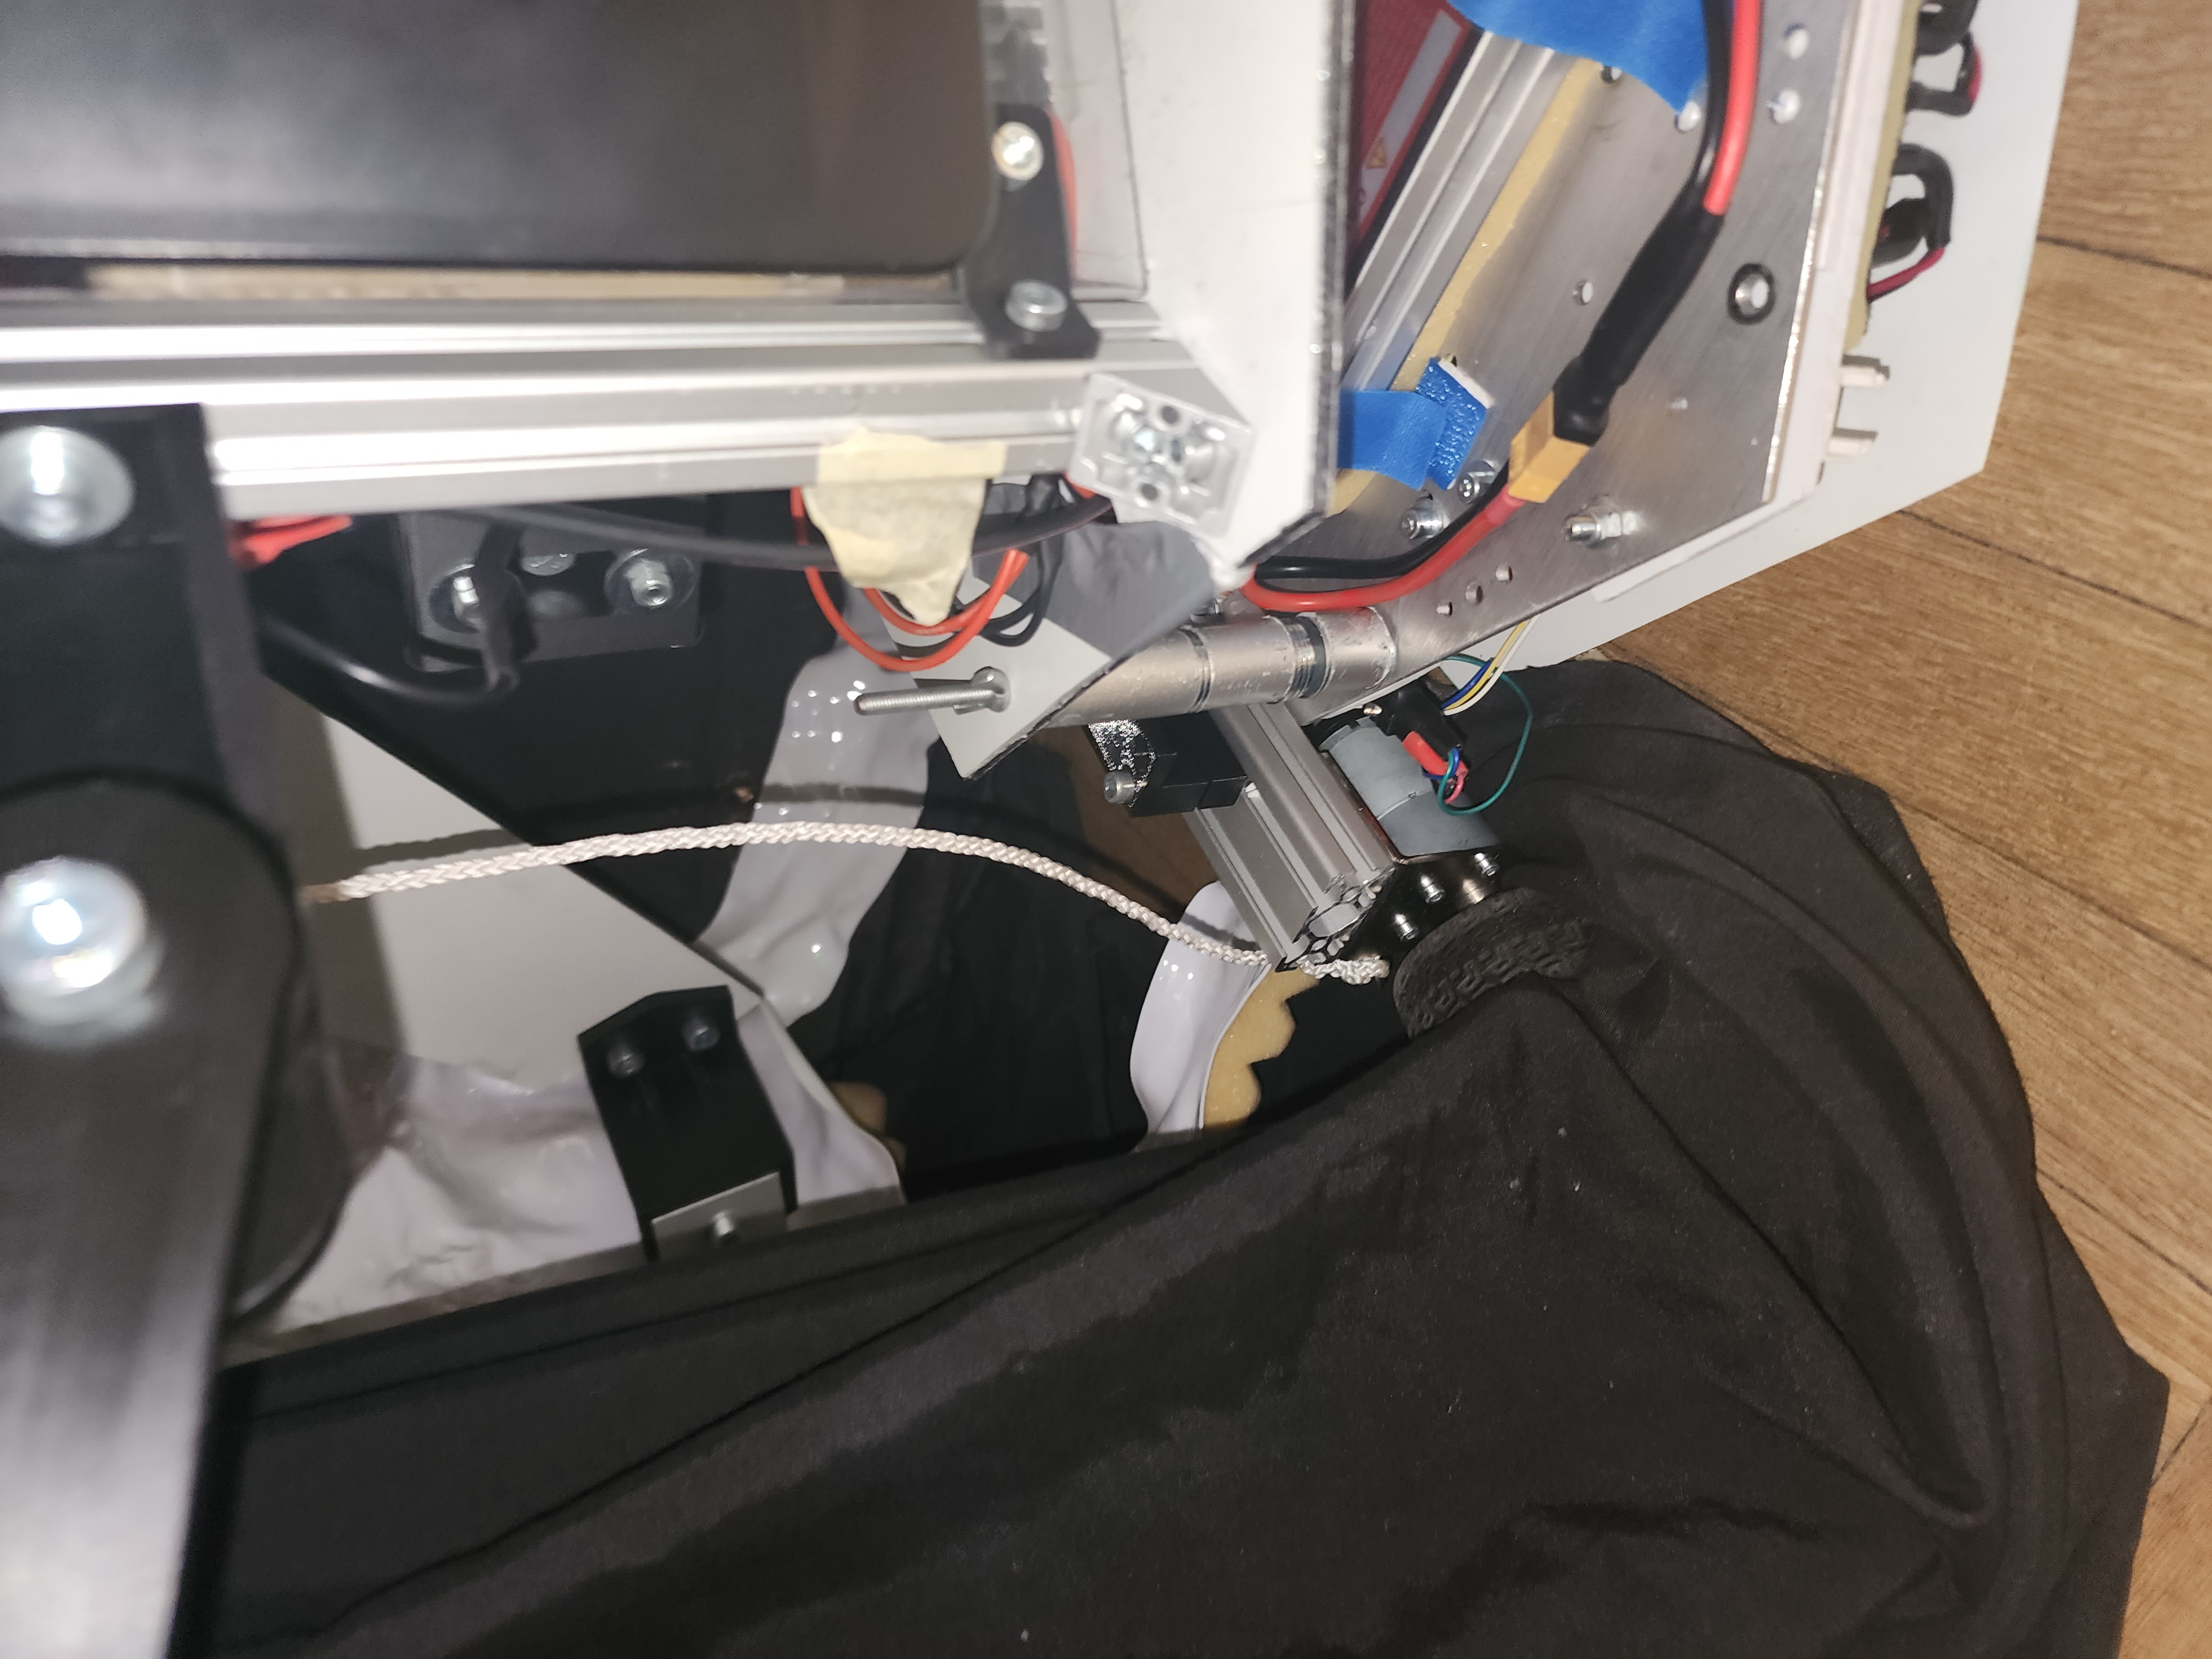
\includegraphics[height=6cm,angle=-90]{Images/WheelVSFabric (2).jpg}
    \caption{Wheel vs Fabric Interference}
    \label{fig:wheel_vs_fabric}
\end{figure}

\begin{figure}[H]
    \centering
    \begin{minipage}{0.45\textwidth}
        \centering
        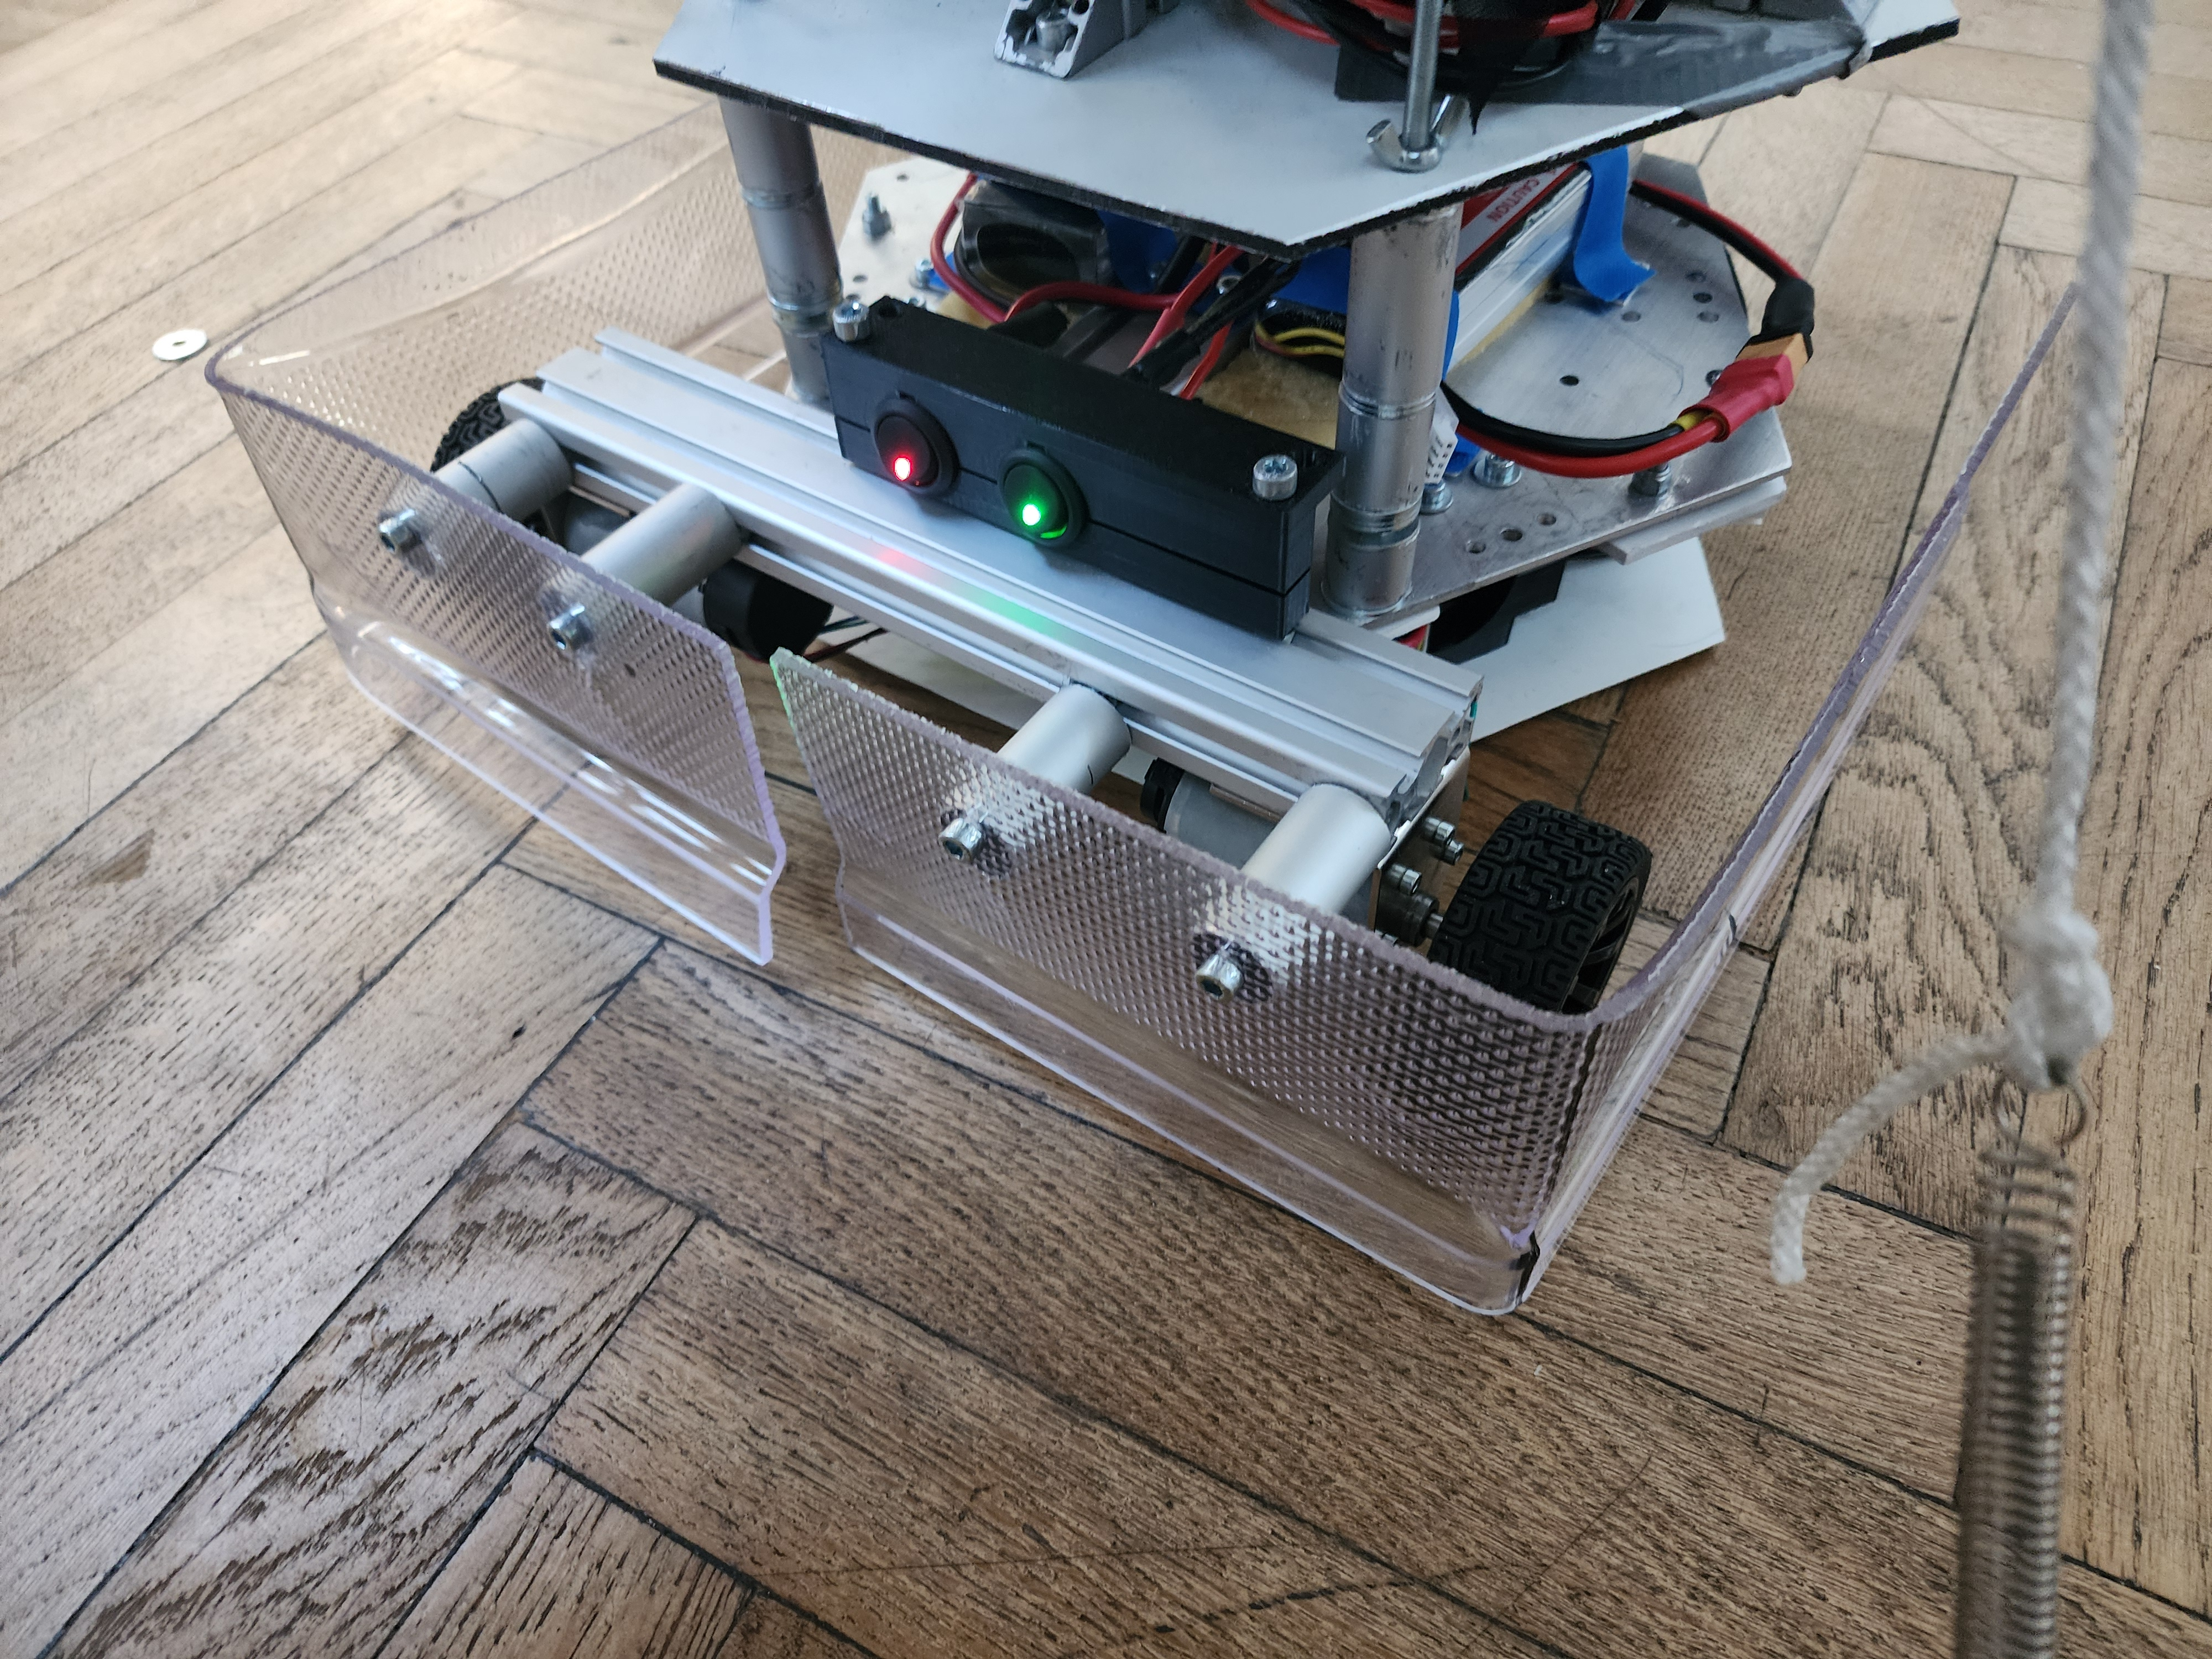
\includegraphics[width=\textwidth]{Images/TinoBumper (4).jpg}
        \caption{Tino Bumper Front View}
        \label{fig:tino_bumper_front}
    \end{minipage}
    \hfill
    \begin{minipage}{0.45\textwidth}
        \centering
        \includegraphics[width=\textwidth]{Images/TinoBumper (5).jpg}
        \caption{Tino Bumper Top View}
        \label{fig:tino_bumper_top}
    \end{minipage}
\end{figure}

The control system adaptation required comprehensive modification to support differential drive kinematics while maintaining compatibility with existing command interfaces. A custom PID controller was developed specifically for differential drive characteristics, replacing the VirHas library with optimized algorithms utilizing Kp=7.3, Ki=5.6, and Kd=0.2 parameters tuned for MDD10A motor drivers. Motor speed calculation employs encoder feedback with 1920 pulses per revolution (PPR) encoders, while atomic movement control integrates four distinct movement states that support synchronized leg-base coordination for VR integration.

\begin{figure}[H]
    \centering    \includegraphics[width=0.8\textwidth, angle=-90]{Images/TinoOnNewBase.jpg}
    \caption{Tino's new Base}
    \label{fig:tino_on_new_base}
\end{figure}

Motor speed calculation employs encoder feedback with 1920 pulses per revolution (PPR) encoders through the \texttt{getMotorSpeed()} function, enabling closed-loop speed control for precise movement execution. The \texttt{updatePid()} function implements the complete PID algorithm with integral term reset, derivative damping, and output limiting to ±255 PWM range, ensuring stable motor control without oscillation.

The \texttt{updateBaseMovementByTime()} function manages four distinct movement states that implement atomic operation completion where each movement phase must finish before accepting new commands. This prevents interrupted motions that could compromise synchronized robot behavior during VR integration. With the kinematic base providing reliable mobility, the system required enhanced power delivery capabilities to support the computational demands of the upgraded processing platform.

\subsection{Power Supply System}

The transition from Raspberry Pi to NVIDIA Orin Nano necessitated complete power system redesign to support significantly higher computational loads and multiple high-performance components. The legacy Raspberry Pi power distribution system proved inadequate for the Orin Nano's 19V DC requirement, Oak-D Pro camera power demands, and enhanced router system, requiring comprehensive architecture overhaul with consolidated battery management and efficient DC-DC conversion.

\subsubsection{System Requirements and Power Analysis}

The Orin Nano requires 19V DC input with power consumption reaching up to 2A during maximum computational load scenarios including simultaneous SLAM processing, human detection, audio processing, and ROS2 node operation. Typical operational consumption ranges between 1.3A to 1.4A during standard social interaction scenarios, with peak consumption of 38W during maximum load conditions and sustained operation typically requiring 25--27W. The power profile exhibits significant variation based on computational load, requiring robust power delivery capable of handling transient peaks without voltage drop.

Auxiliary system requirements include the Oak-D Pro camera system requiring 5V DC input with power consumption up to 5W during high-resolution stereo processing, and the onboard router system requiring 5V DC input with approximately 3W consumption during operational periods. Total system power budget analysis indicates maximum power consumption of approximately 46W under peak operational conditions, with typical sustained operation requiring 33--35W.

\subsubsection{Power Conversion and Distribution Implementation}

The power conversion system utilizes high-efficiency DC-DC converters to transform battery voltage to the multiple voltage levels required by system components. The Oumefar DC-DC step-up converter provides stable 19V output from 12V battery input with efficiency ratings exceeding 85\% across the operational load range, with converter selection prioritizing stability, efficiency, and thermal performance under sustained loading conditions. Power delivery stability testing demonstrated consistent voltage regulation within ±2\% across full load range with excellent transient response during computational load variations.

The 12V to 5V conversion system provides power for auxiliary components including the Oak-D Pro camera and onboard router, with power distribution architecture enabling independent power control for auxiliary components. 

\subsubsection{Battery System Consolidation and Performance}

The battery system redesign consolidates multiple power sources while providing enhanced capacity and reliability for extended operational periods. The primary battery system utilizes 5200mAh 80C 11.1V 57.72Wh LiPo batteries that provide the power density and discharge capabilities required for robotic applications, with battery specification analysis demonstrating adequate capacity for 2--3 hours of typical operation with conservative discharge management.

Maximum load operational time calculations indicate approximately 1.37 hours of operation under peak power conditions, though realistic operational scenarios typically achieve 2+ hours due to variable computational loading. The high discharge rate capability (80C) ensures stable power delivery during computational peaks without voltage sag, while the system consolidation reduces complexity from four separate battery systems to three integrated power sources.

The cable harness redesign eliminates obsolete USB-A and USB-C connections utilized for Raspberry Pi power delivery, replacing them with proper 12V distribution and 19V DC jack connectivity optimized for Orin Nano requirements. The 12V input distribution system provides primary power for both the step-up converter and the secondary 5V converter, with the 19V DC jack implementation providing secure power connection to the Orin Nano with proper mechanical support and electrical contact reliability.
% REORG_TAG: moved here from Stewart Platform Head Mechanism Improvements
\subsection{Stewart Platform Head Mechanism}

The Stewart platform head mechanism required iterative design improvements to address systematic reliability issues encountered during extended operational periods. The original implementation exhibited servo axis misalignment that created excessive stress concentrations on servo motor internals during head movement operations, with force analysis revealing that head loads were transmitted directly through servo shafts rather than through the structural framework. Additionally, the connecting arms showed excessive structural flexibility that reduced head positioning precision and contributed to mechanical instability, with repeated arm failures occurring due to inadequate load distribution and material selection in the 3D printed PLA components.

\begin{figure}[H]
    \centering
    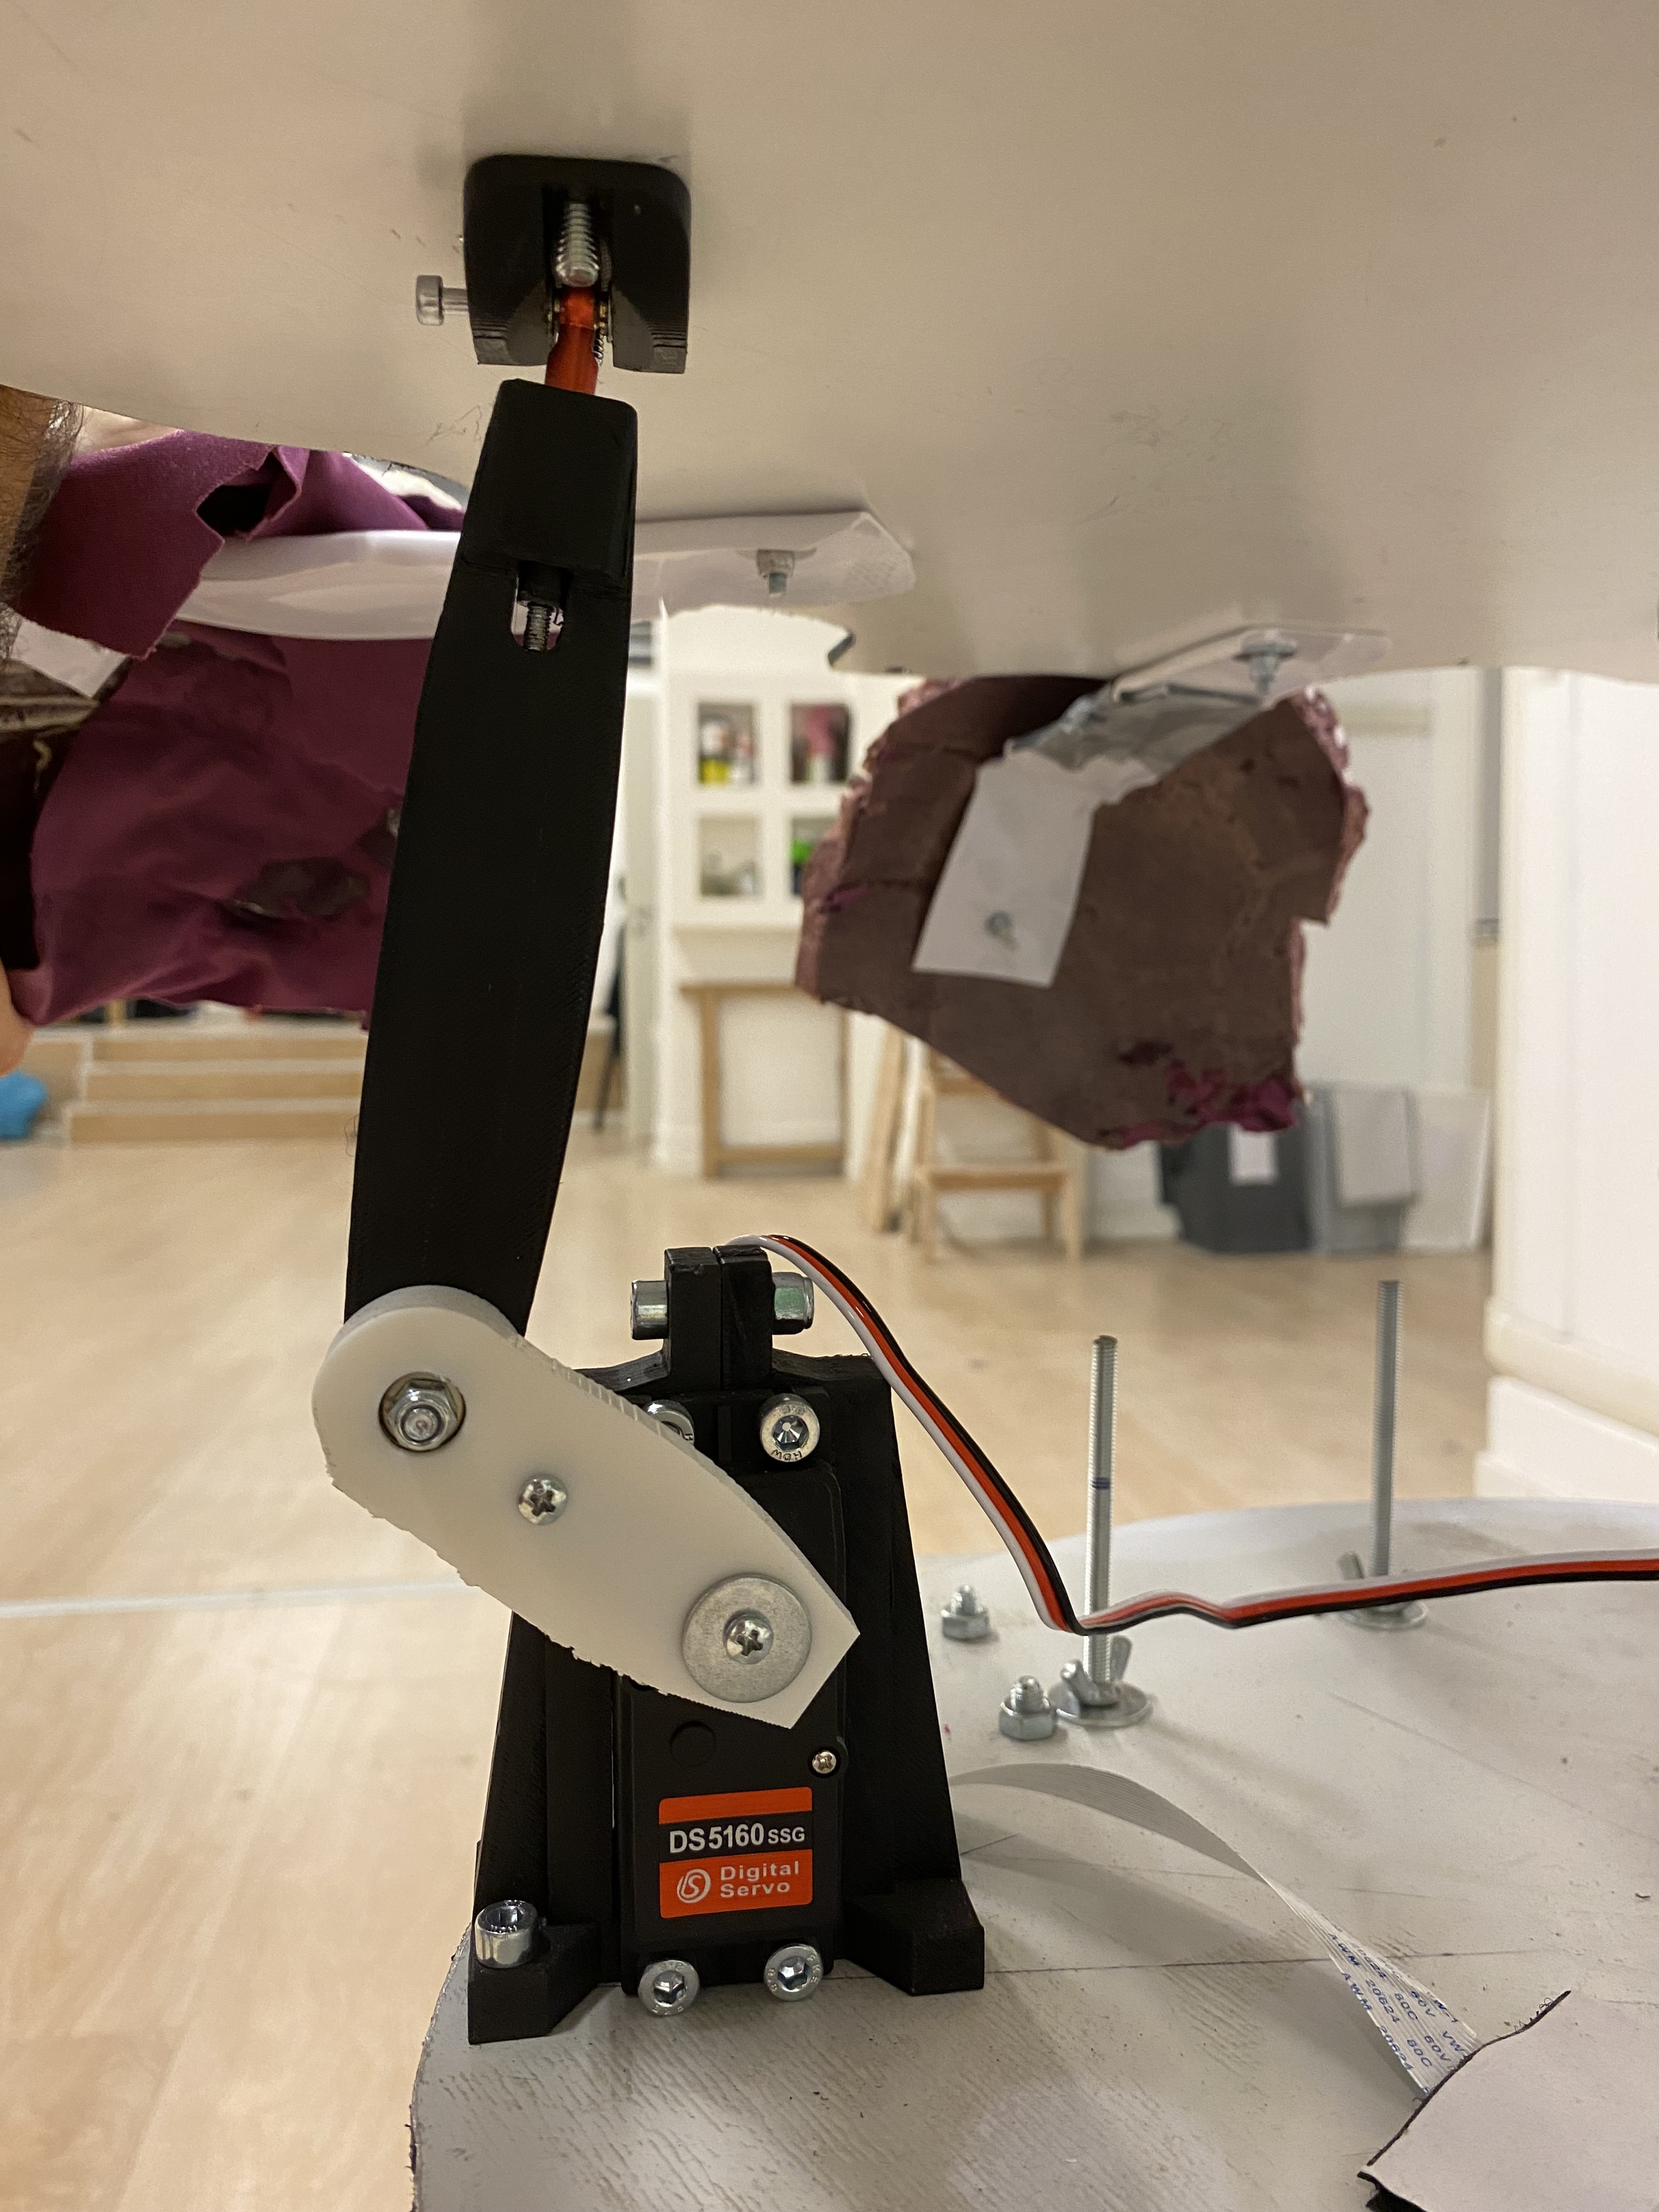
\includegraphics[height=6cm]{Images/signle_head_motor.jpg}
    \caption{Head Arm V0 Design}
    \label{fig:head_arm_v0}
\end{figure}

\subsubsection{Design Evolution and Failure Resolution}

The first design iteration focused on servo axis alignment to redirect forces through proper load paths while maintaining the existing bearing-based connection system. The servo axis alignment improvement redirected head loads through the structural framework rather than servo mechanisms, with enhanced PLA arm geometry providing improved load distribution through optimized cross-sectional design and stress concentration reduction.

\begin{figure}[H]
    \centering
    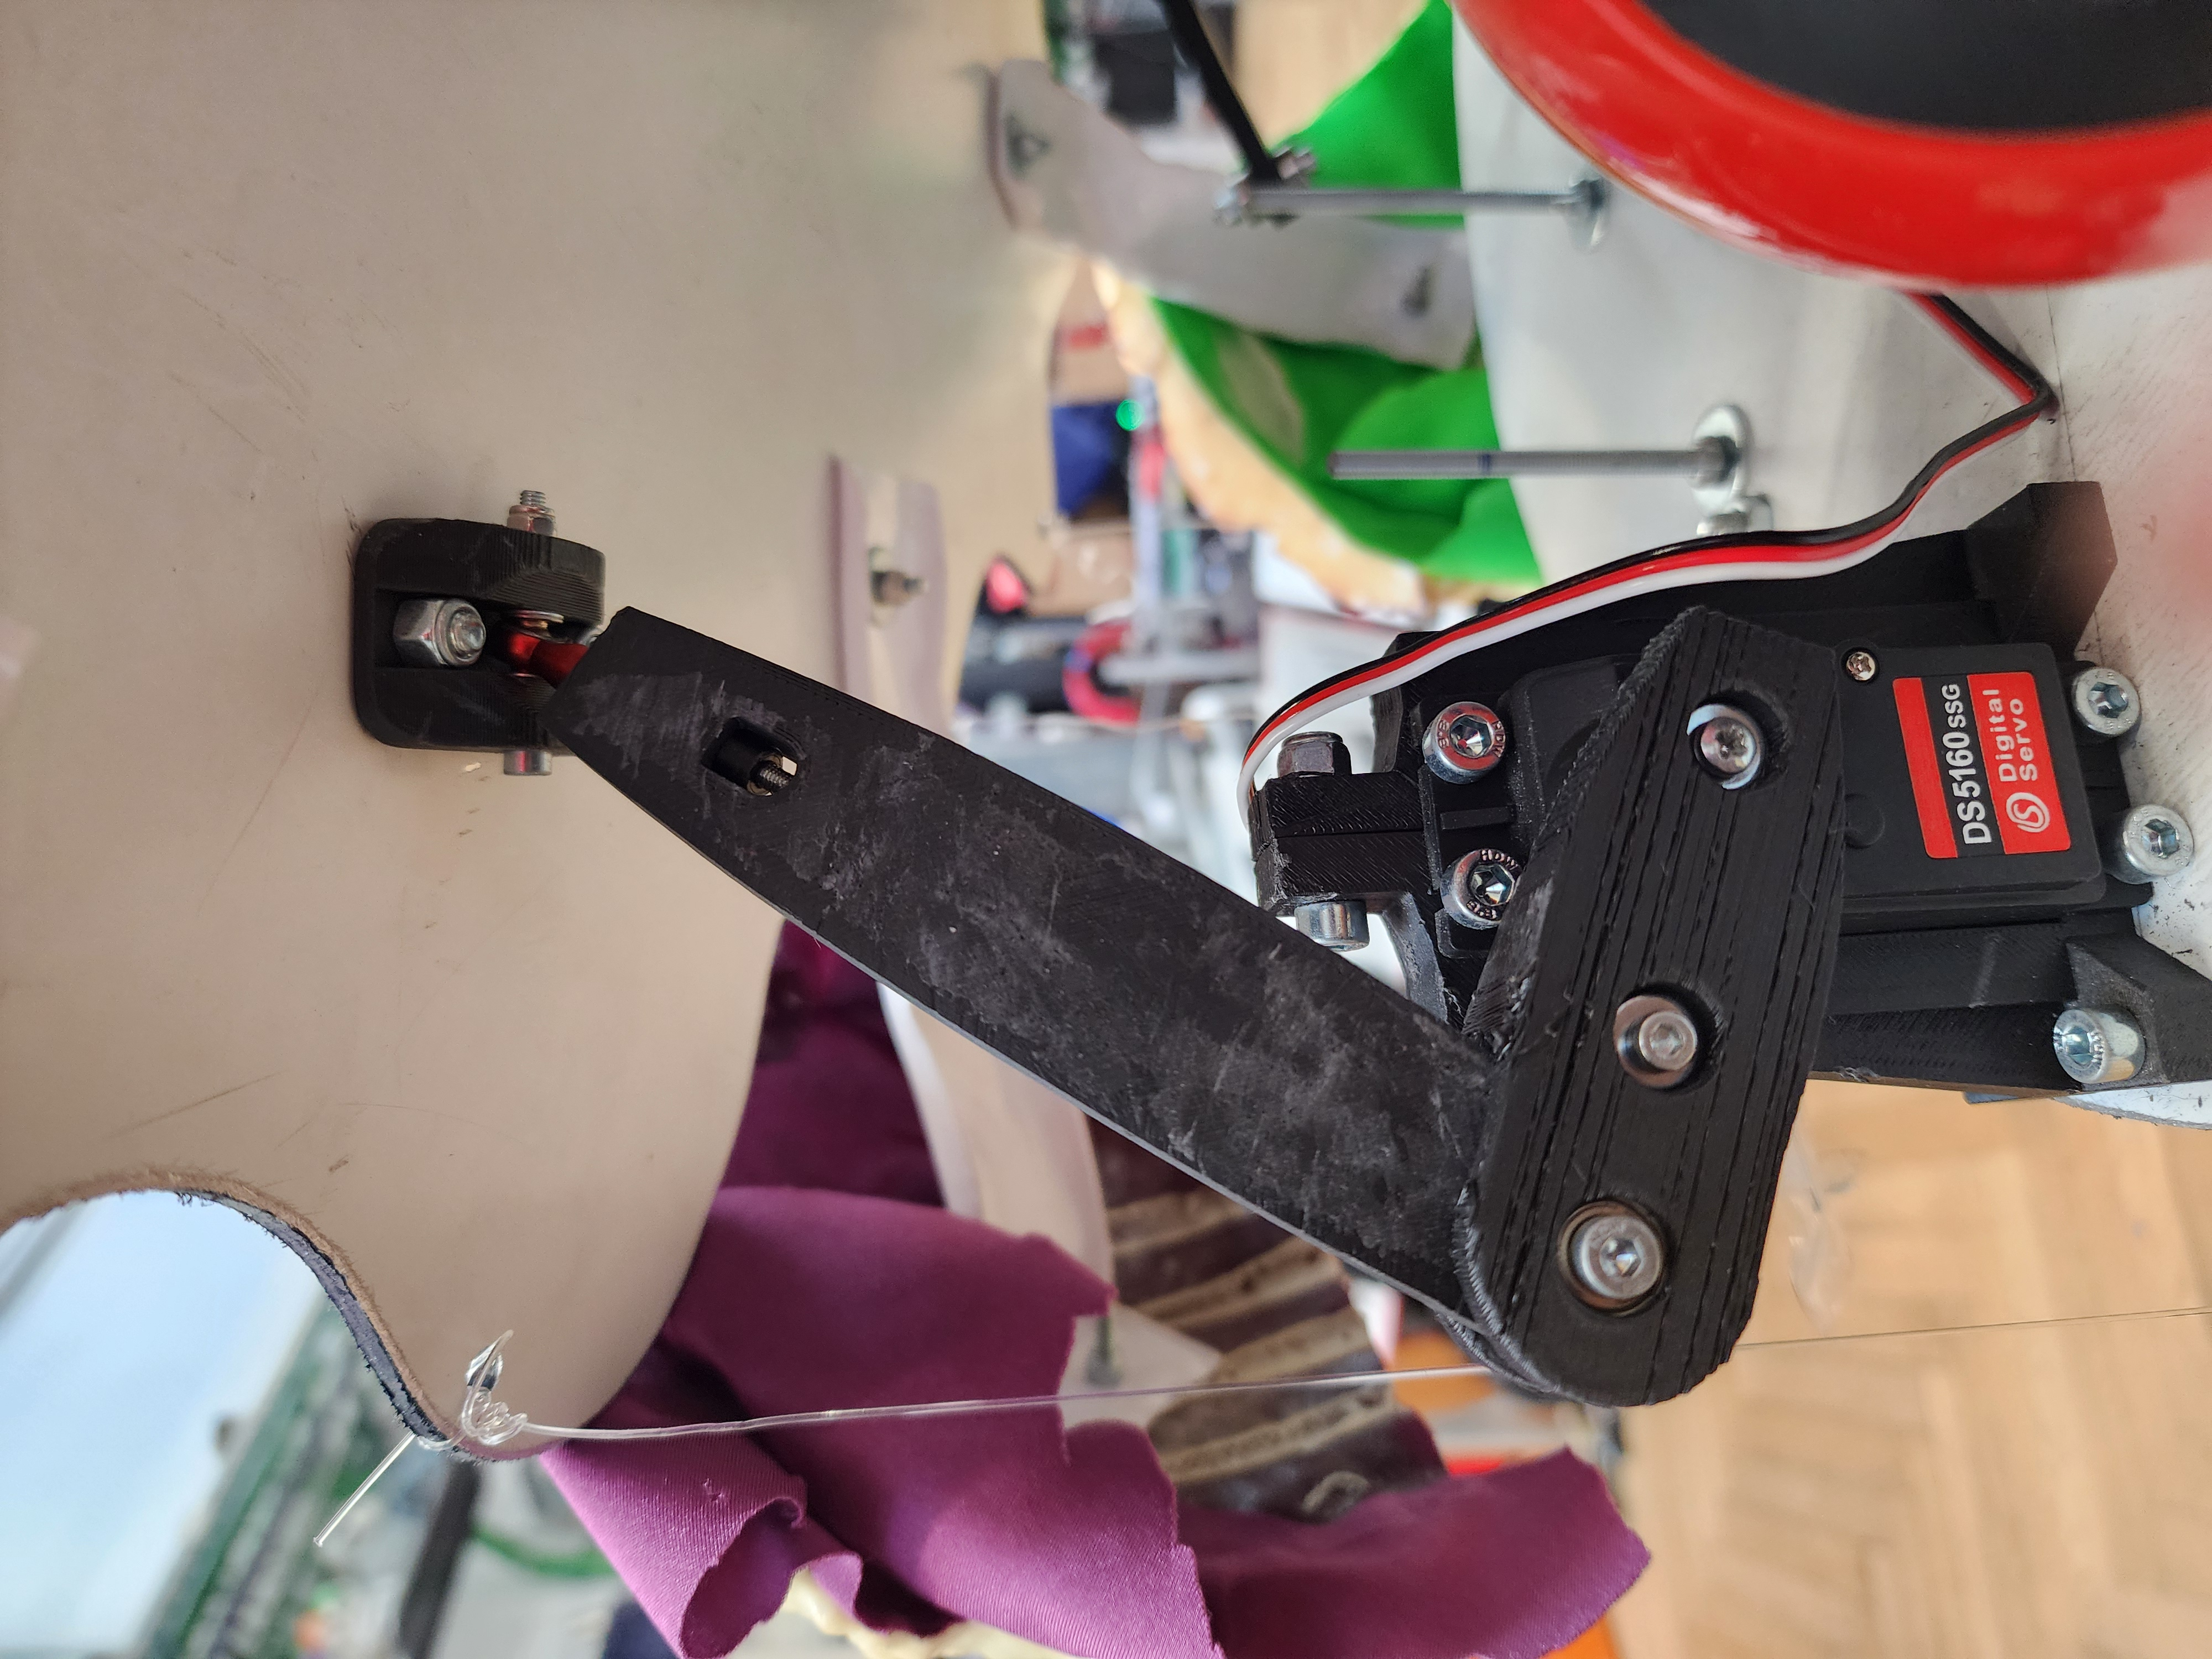
\includegraphics[height=6cm, angle=-90]{Images/HeadArmV2.jpg}
    \caption{Head Arm V1 Design}
    \label{fig:head_arm_v1}
\end{figure}

Performance evaluation demonstrated reduced servo stress indicators and improved movement precision, though structural flexibility issues remained due to the retained bearing connection system. Despite these improvements, the Stewart platform continued to experience significant structural flexibility problems that led to repeated arm failures during extended operational periods.

\begin{figure}[H]
    \centering
    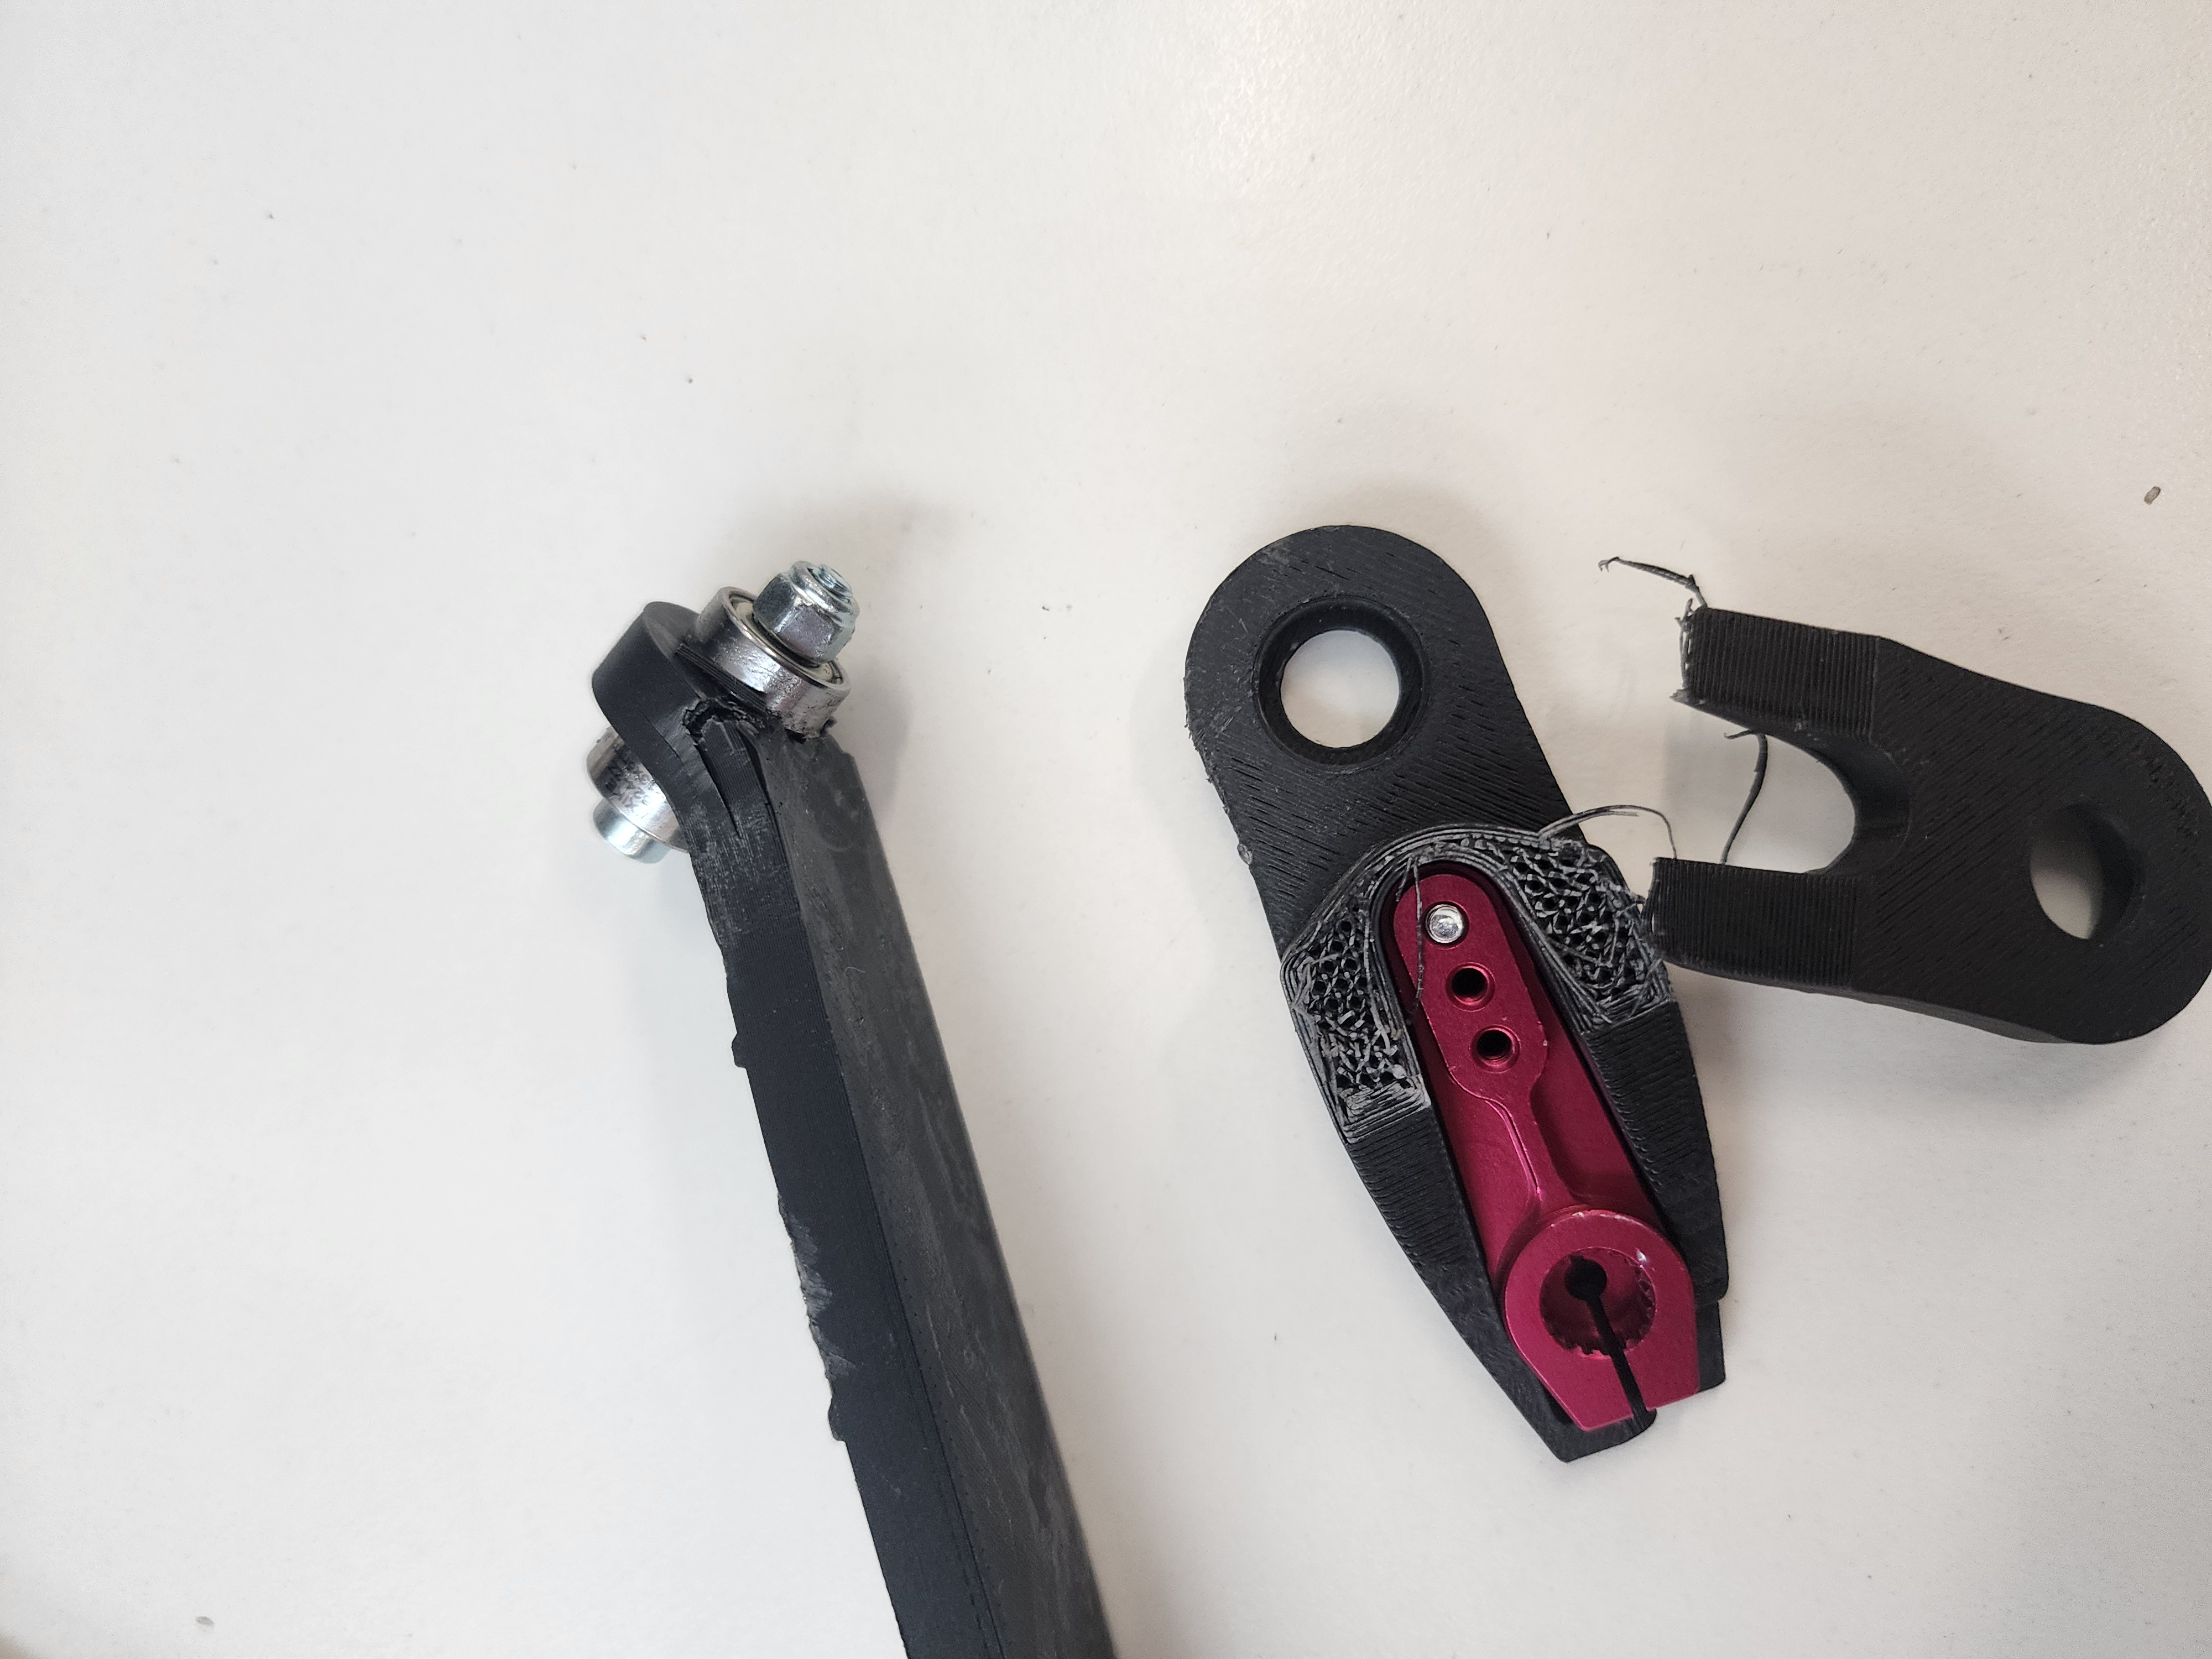
\includegraphics[height=6cm, angle=-90]{Images/HeadArmFailure (2).jpg}
    \caption{Head Arm Failure after Extended Use}
    \label{fig:head_arm_failure}
\end{figure}

The bearing connection system on the servo side of each arm introduced excessive compliance that compromised head positioning precision and contributed to continued mechanical instability. Failure analysis revealed that the 3D printed bearing housings could not adequately transfer forces between the improved servo connections and the head platform, with repeated stress cycling causing progressive degradation and eventual structural failure.

\begin{figure}[htbp]
    \centering
    \begin{minipage}{0.45\textwidth}
        \centering
        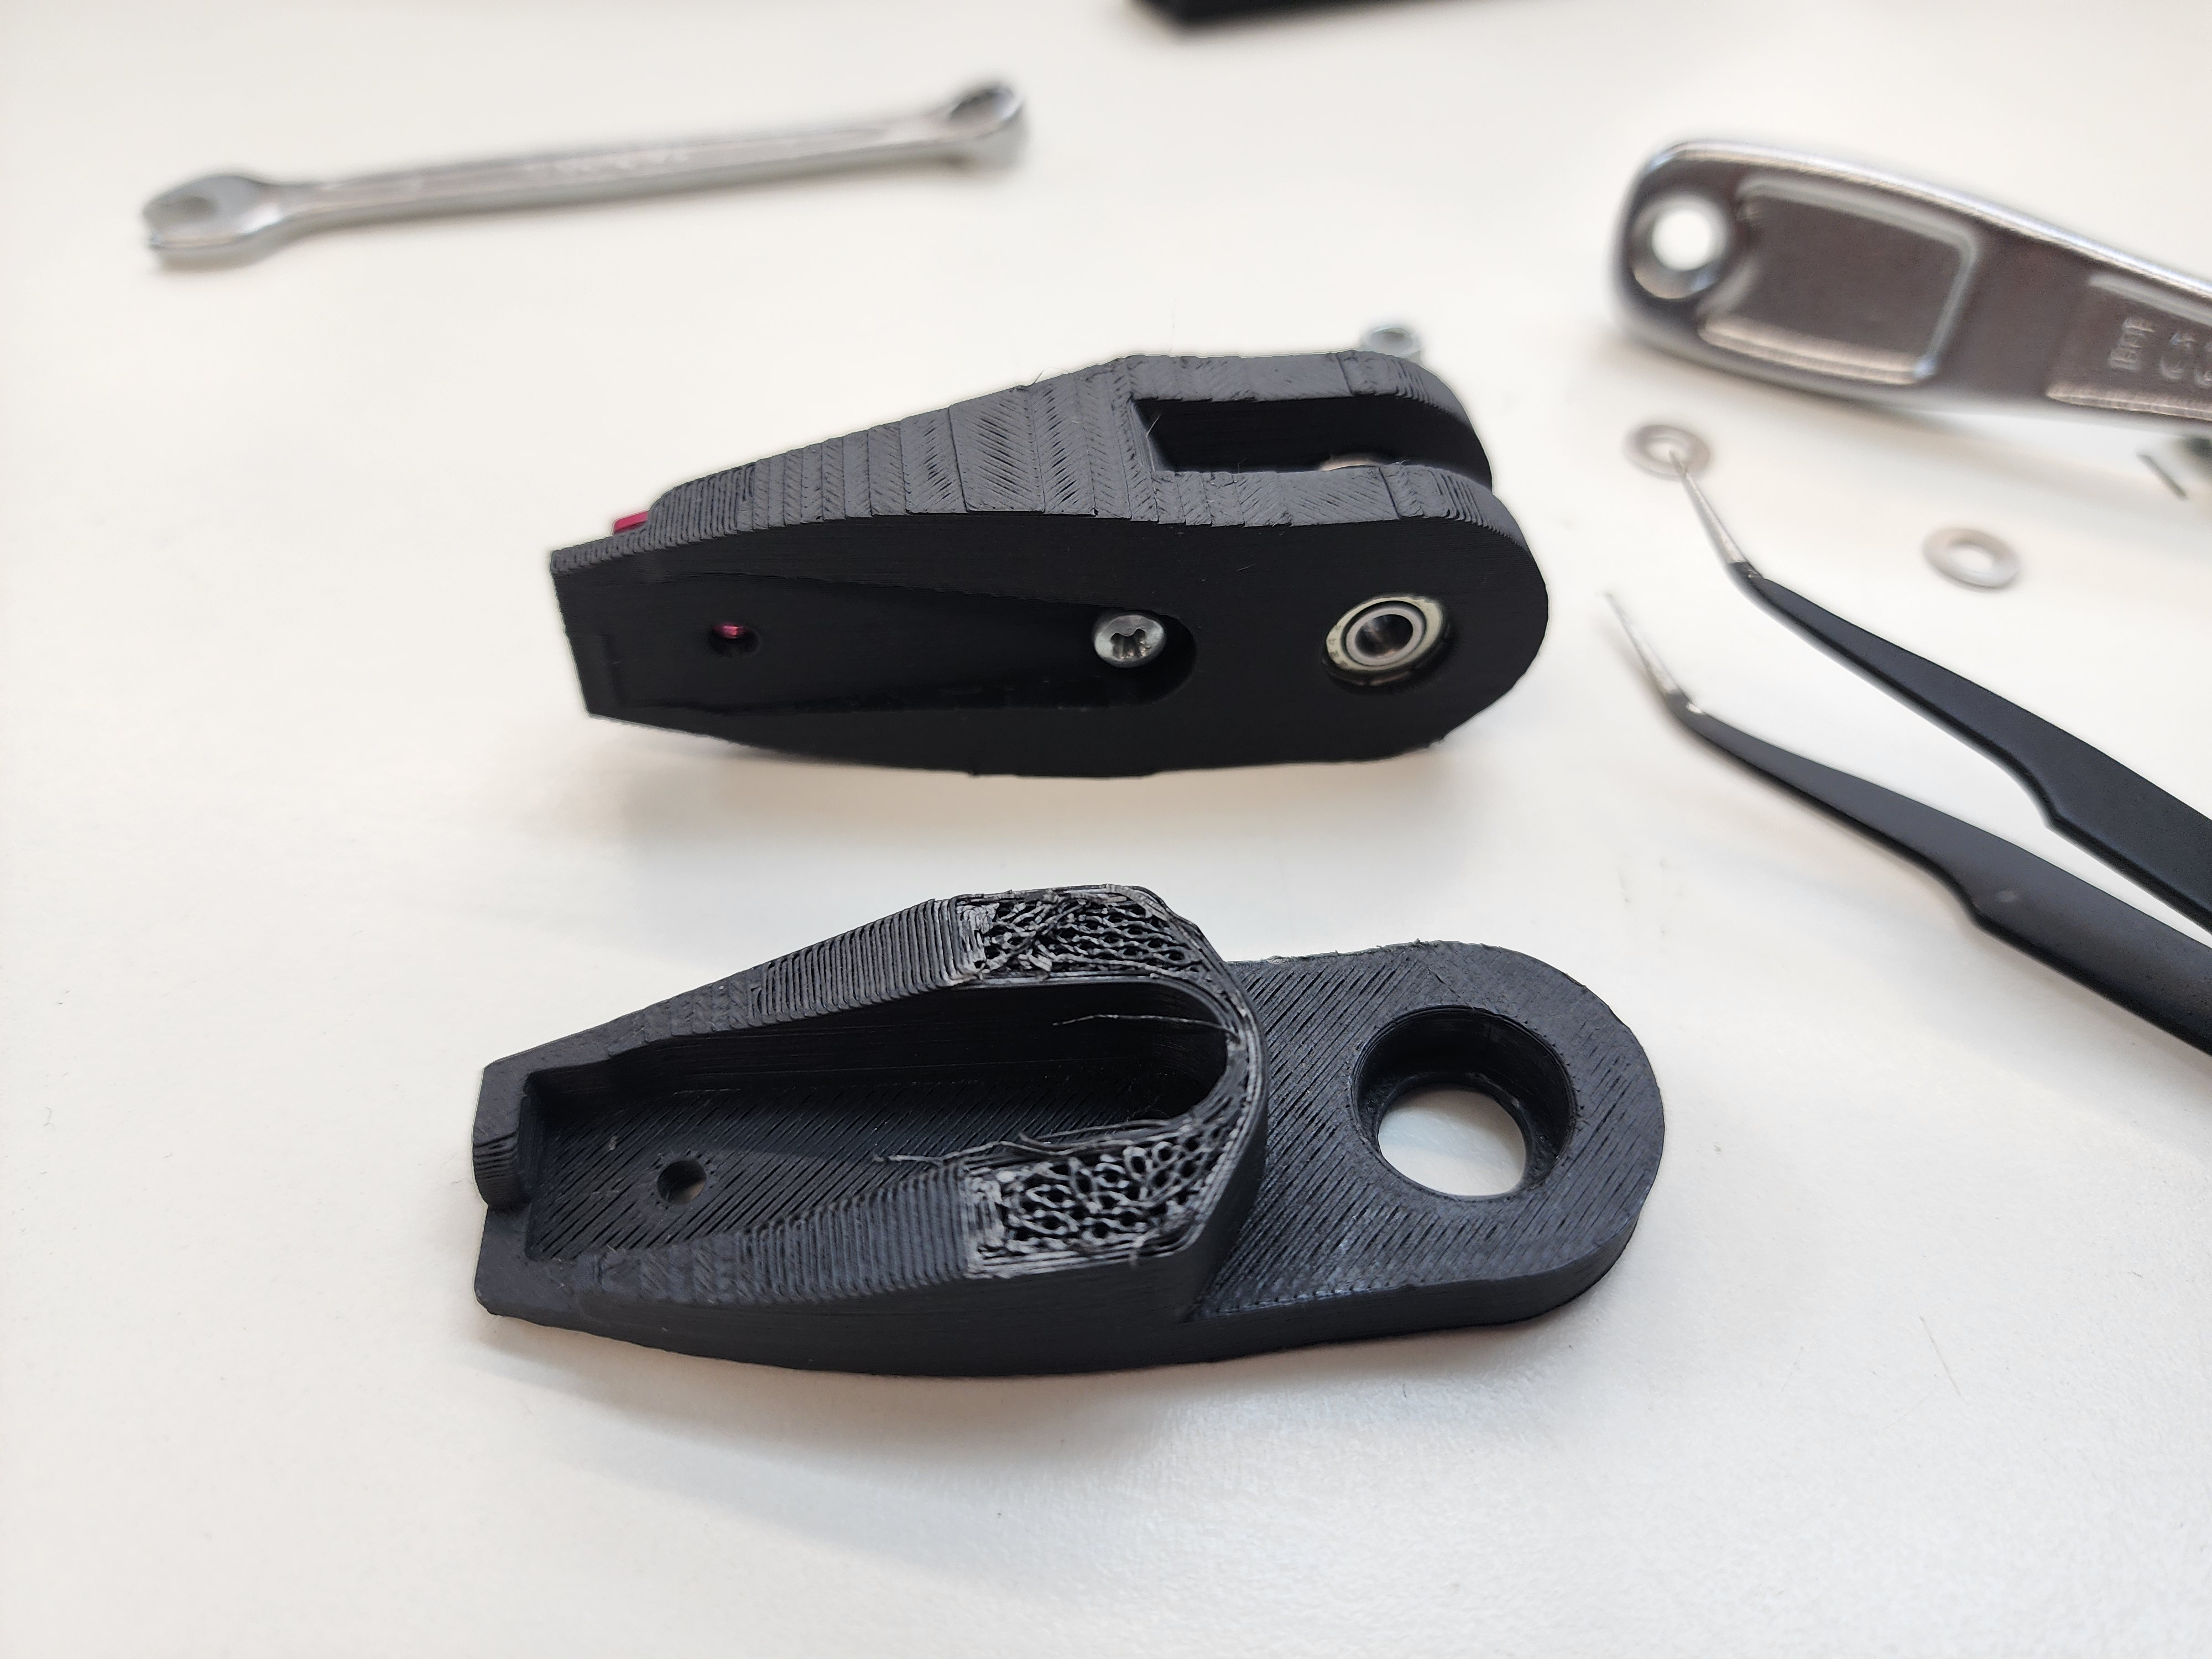
\includegraphics[width=\textwidth]{Images/HeadArmFailure (3).jpg}
        \caption{Servo Side Bearing Connection Failure}
        \label{fig:servo_bearing_failure}
    \end{minipage}
    \hfill
    \begin{minipage}{0.45\textwidth}
        \centering
        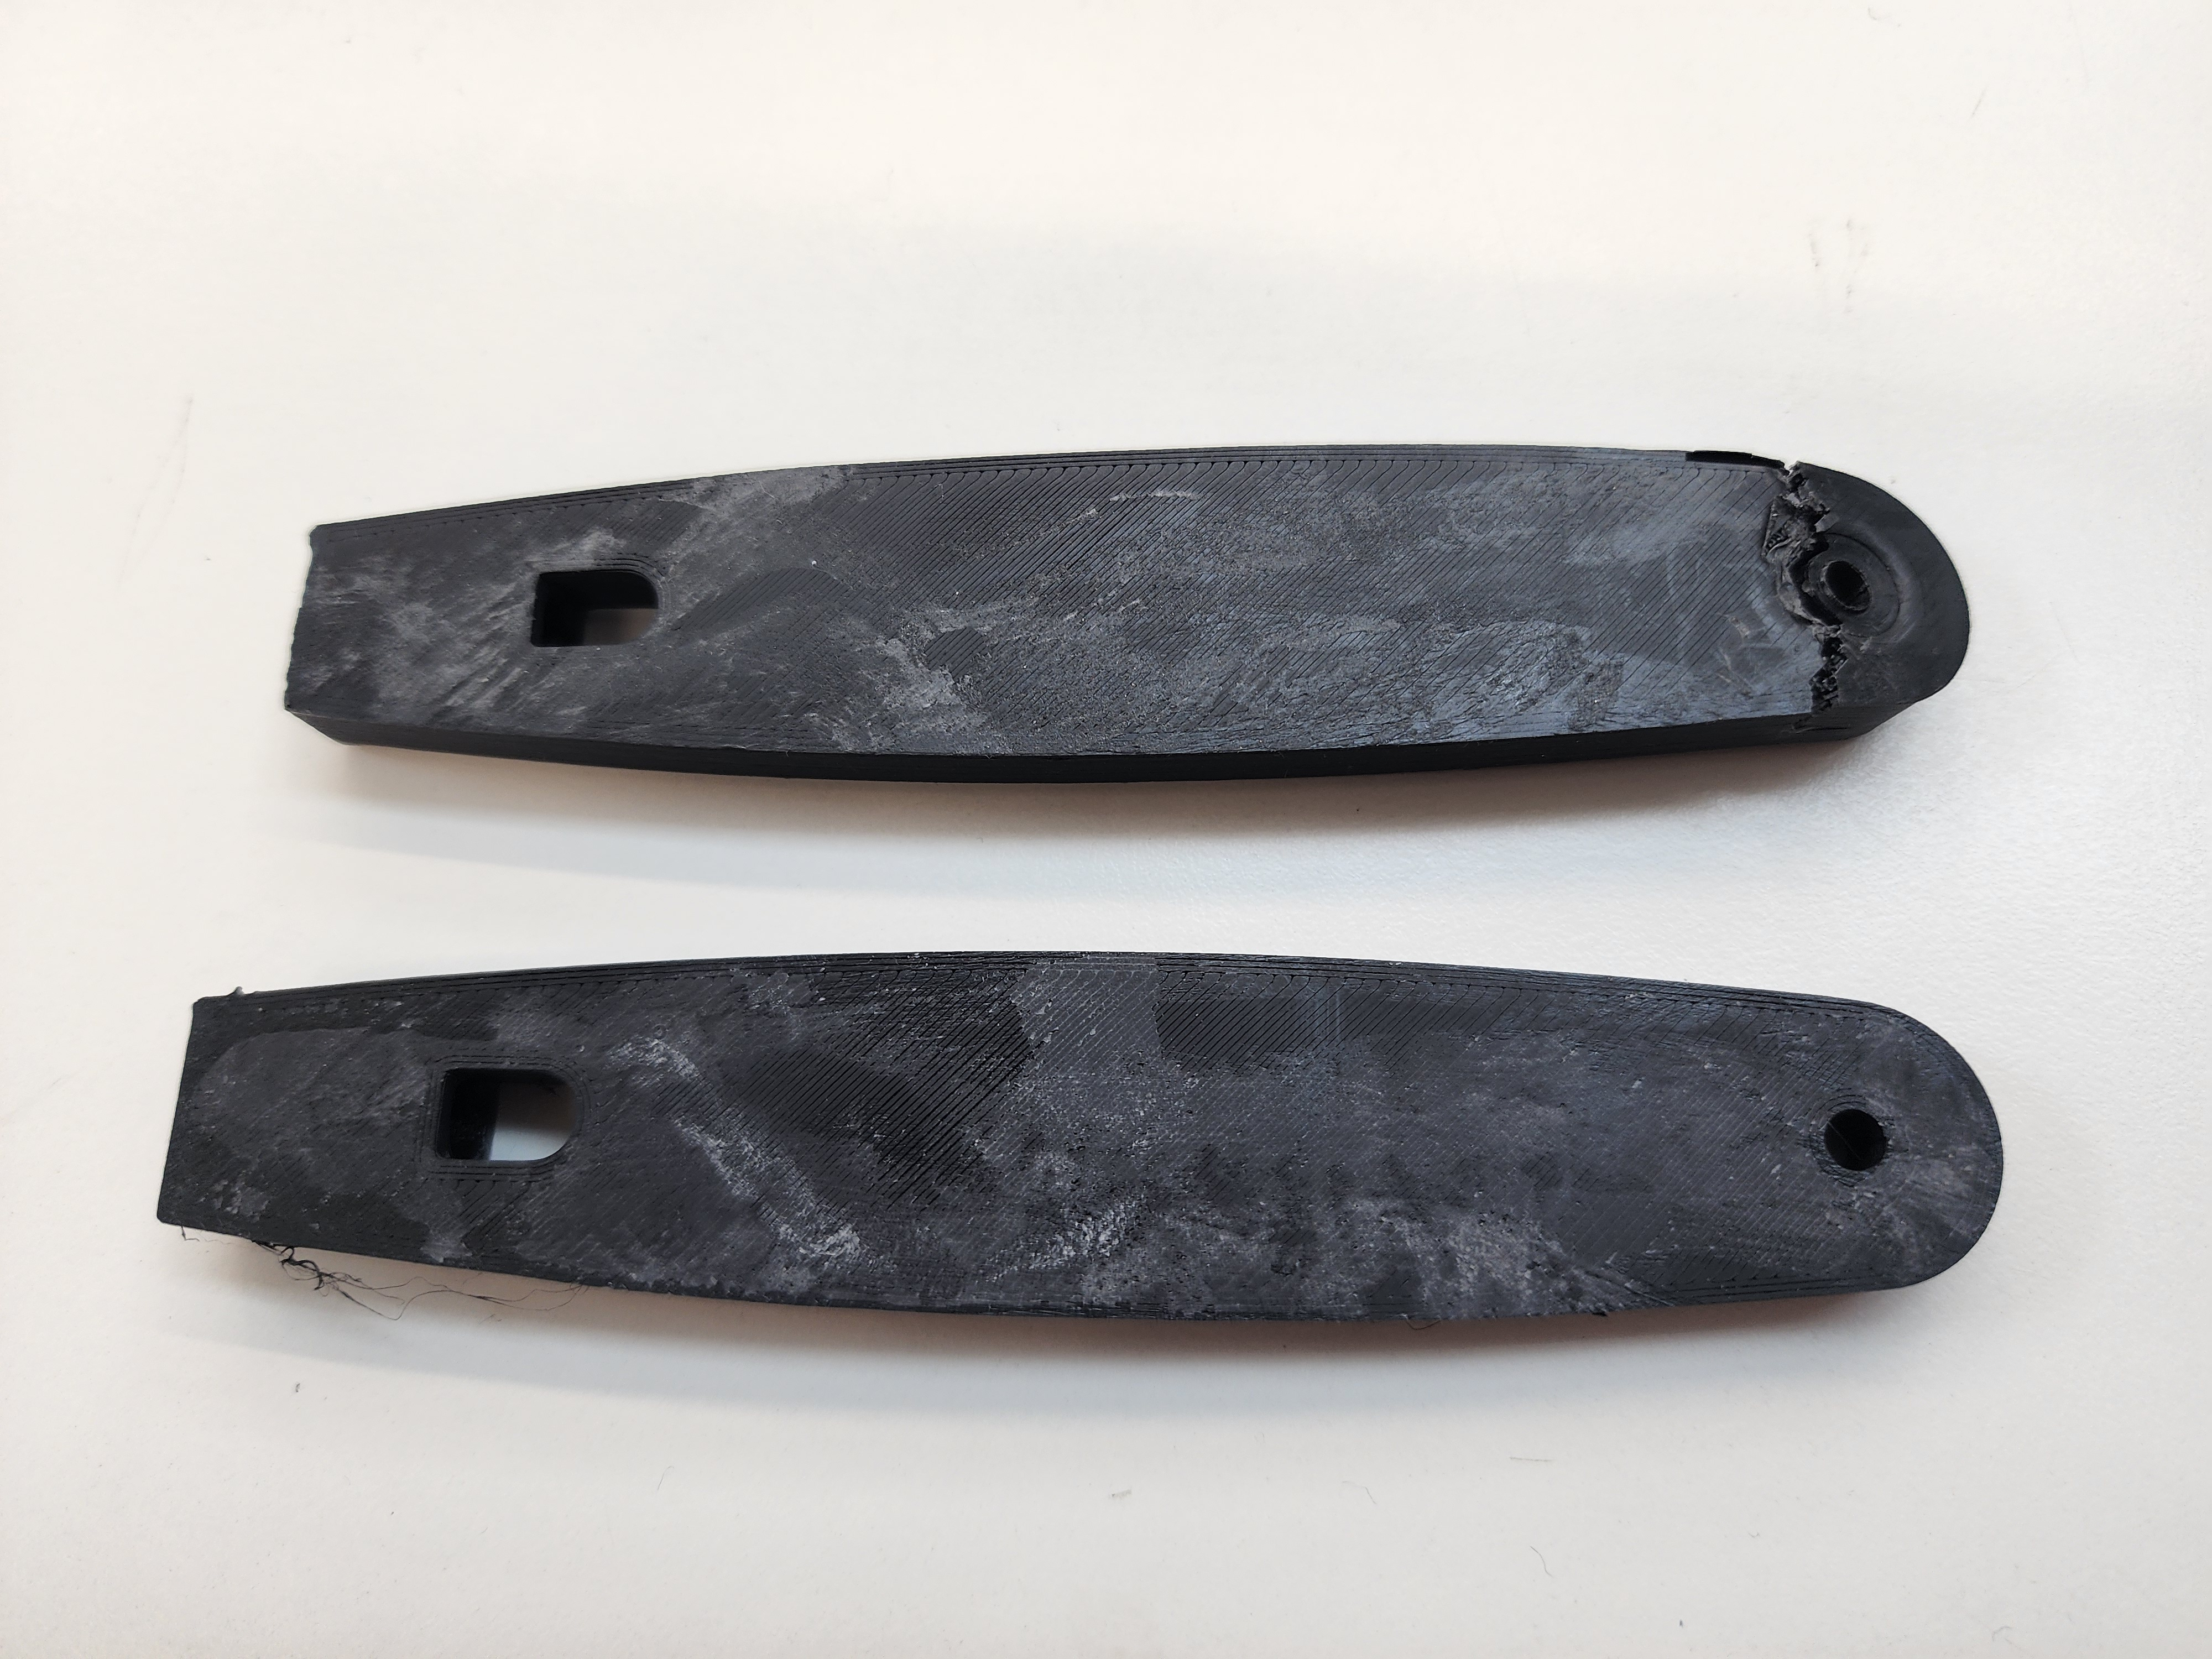
\includegraphics[width=\textwidth]{Images/HeadArmFailure.jpg}
        \caption{Head Arm Failure after Extended Use}
        \label{fig:head_arm_failure_alt}
    \end{minipage}
\end{figure}

\subsubsection{Rod End Solution Implementation}

The fundamental limitation resided in the conflict between smooth articulation requirements and structural rigidity within 3D printed PLA construction constraints. Research into Stewart platform best practices identified rod end connections as the standard solution for eliminating binding while allowing proper articulation throughout the movement range, leading to the final design iteration that adopted rod end (heim joint) connections on both ends of each Stewart platform arm.

\begin{figure}[H]
    \centering
    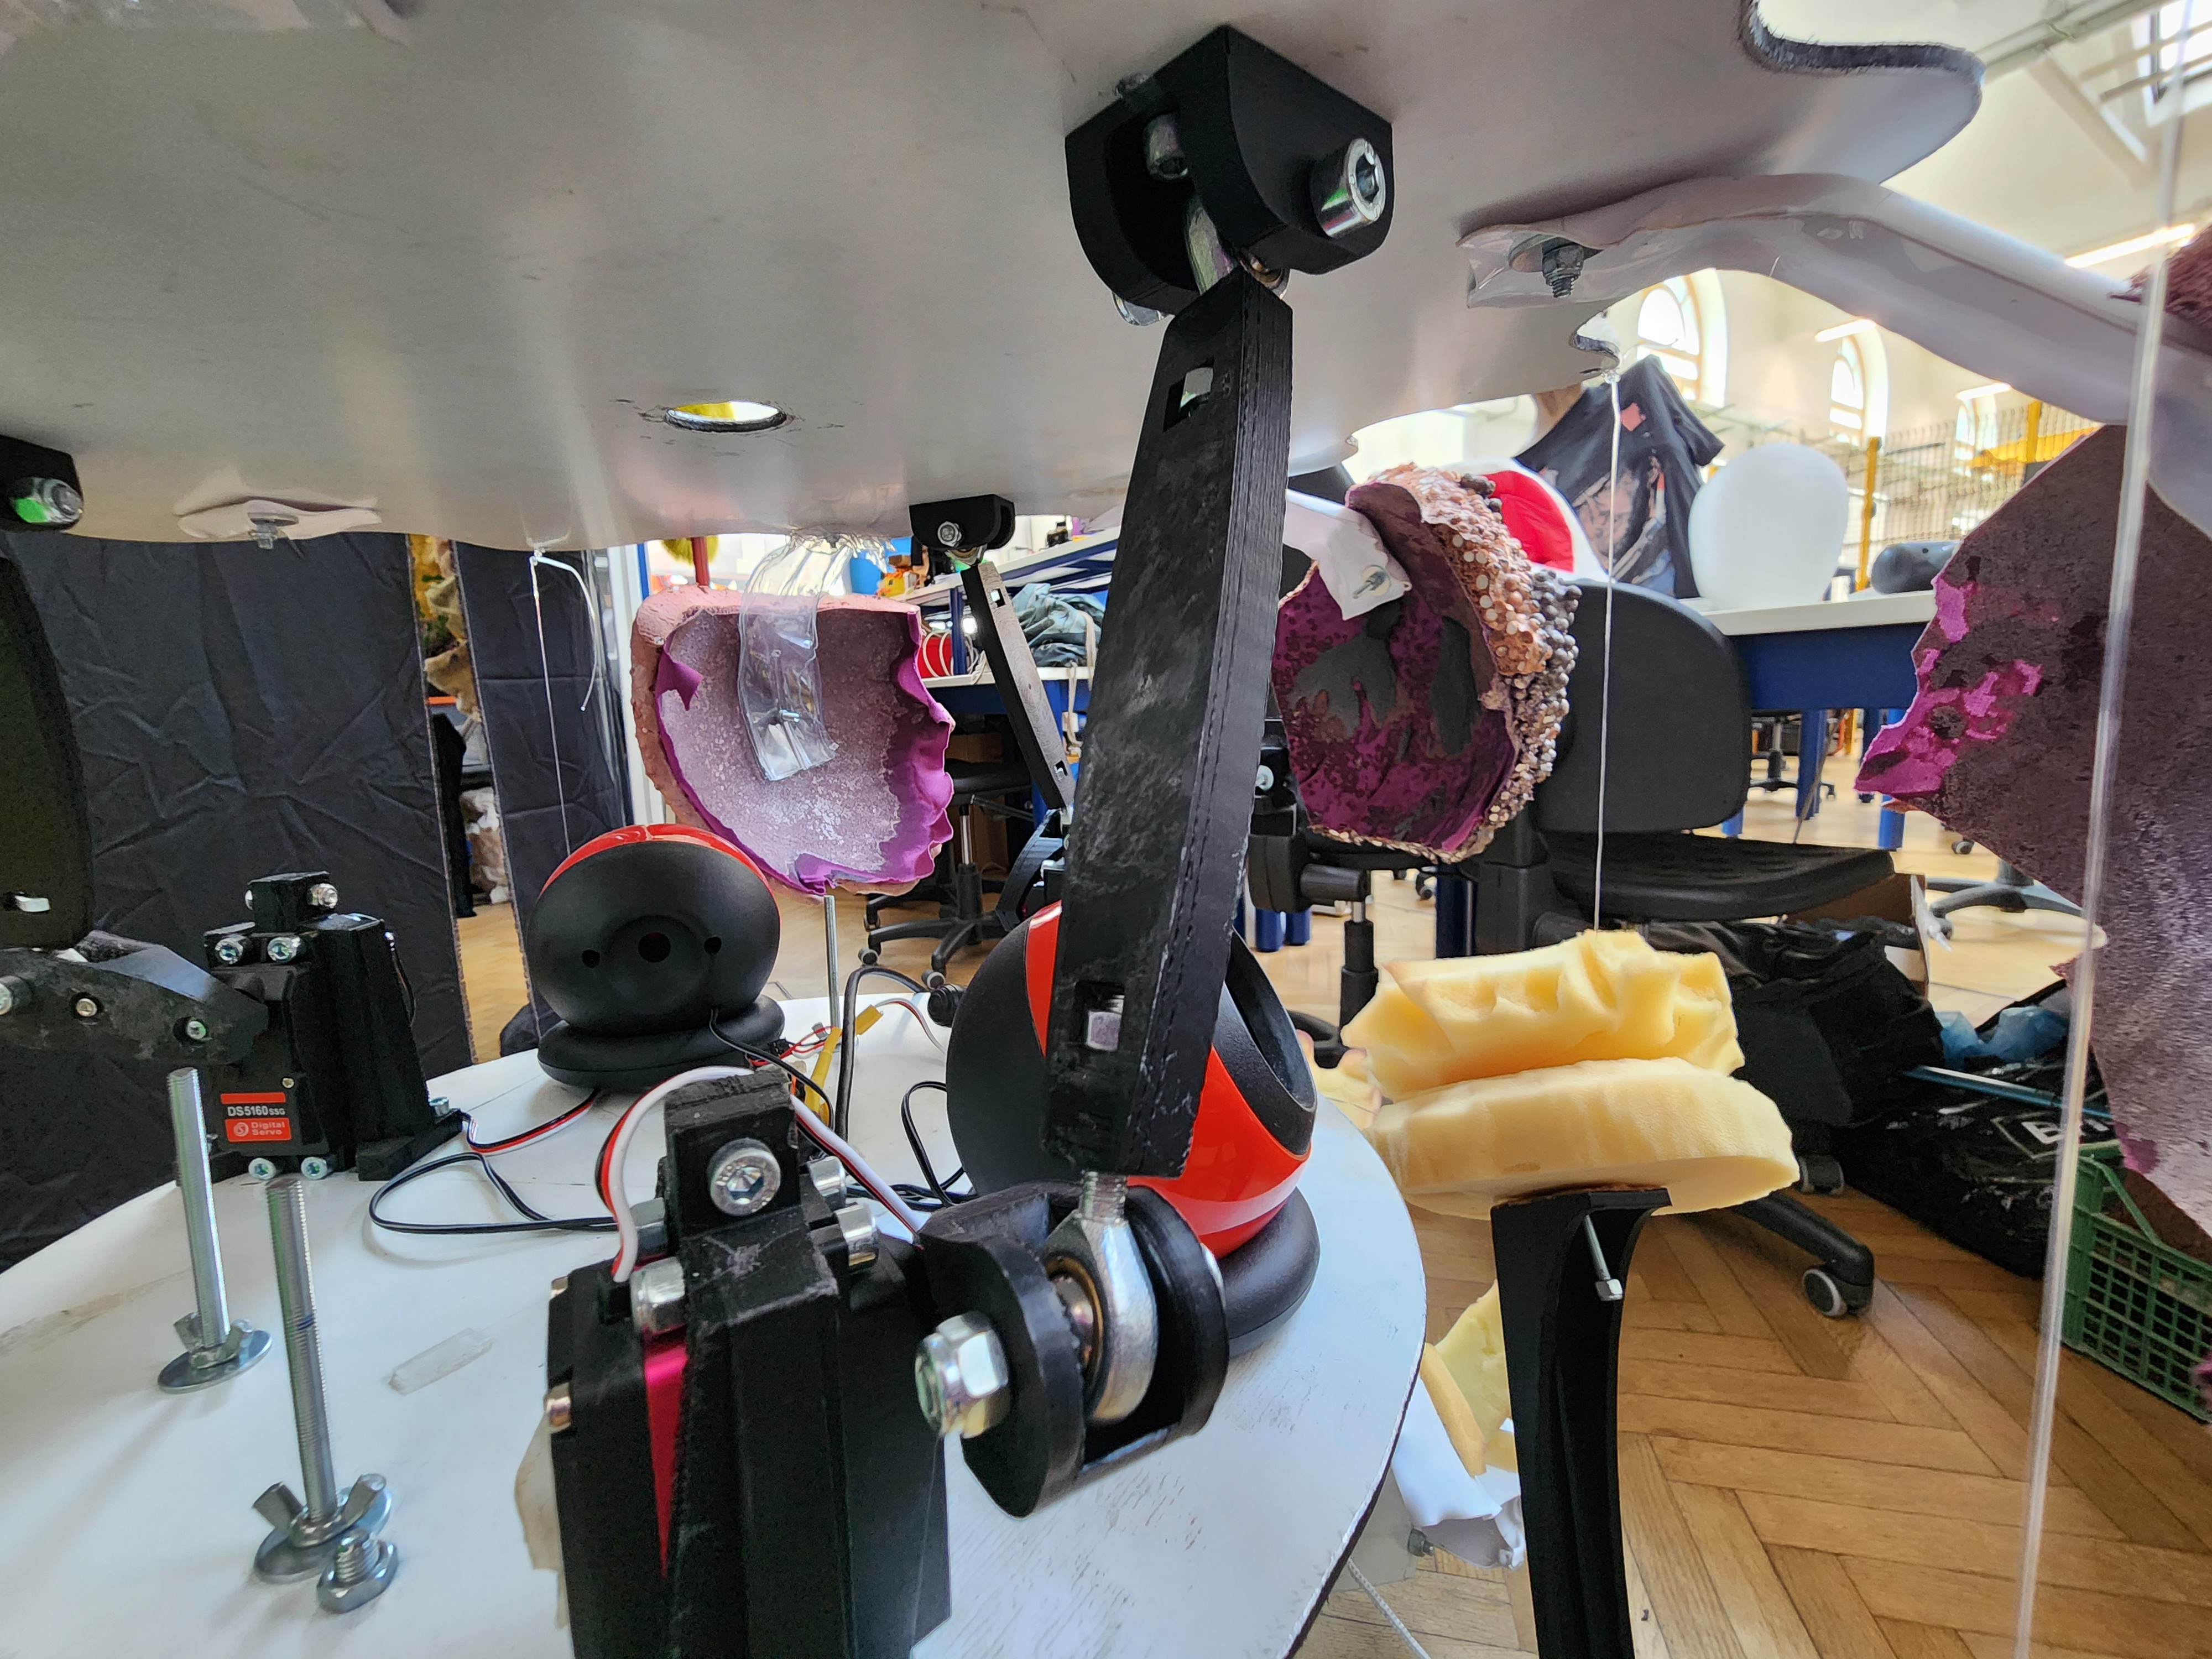
\includegraphics[height=6cm]{Images/NewHeadDoubleJoint (4).jpg}
    \caption{Head Arm V2 Design with Rod Ends}
    \label{fig:head_arm_v2}
\end{figure}

The rod end implementation utilizes metal heim joints that provide superior strength and durability compared to the original bearing system, with metal construction eliminating the brittleness and wear issues encountered with printed bearing housings. Joint articulation characteristics enable free rotation in all necessary axes while providing positive mechanical connection between arm segments, eliminating binding forces that contributed to servo stress and movement precision issues.

Mechanical trade-offs include acceptable head wobble during stationary periods due to free articulation provided by the heim joints, though analysis indicates this wobble may actually enhance Tino's expressive capabilities by providing natural movement characteristics. Structural strength analysis demonstrates significant improvement in mechanical robustness and load-bearing capability while accepting reduced precision during stationary periods.

\begin{figure}[H]
    \centering
    \begin{minipage}{0.45\textwidth}
        \centering
        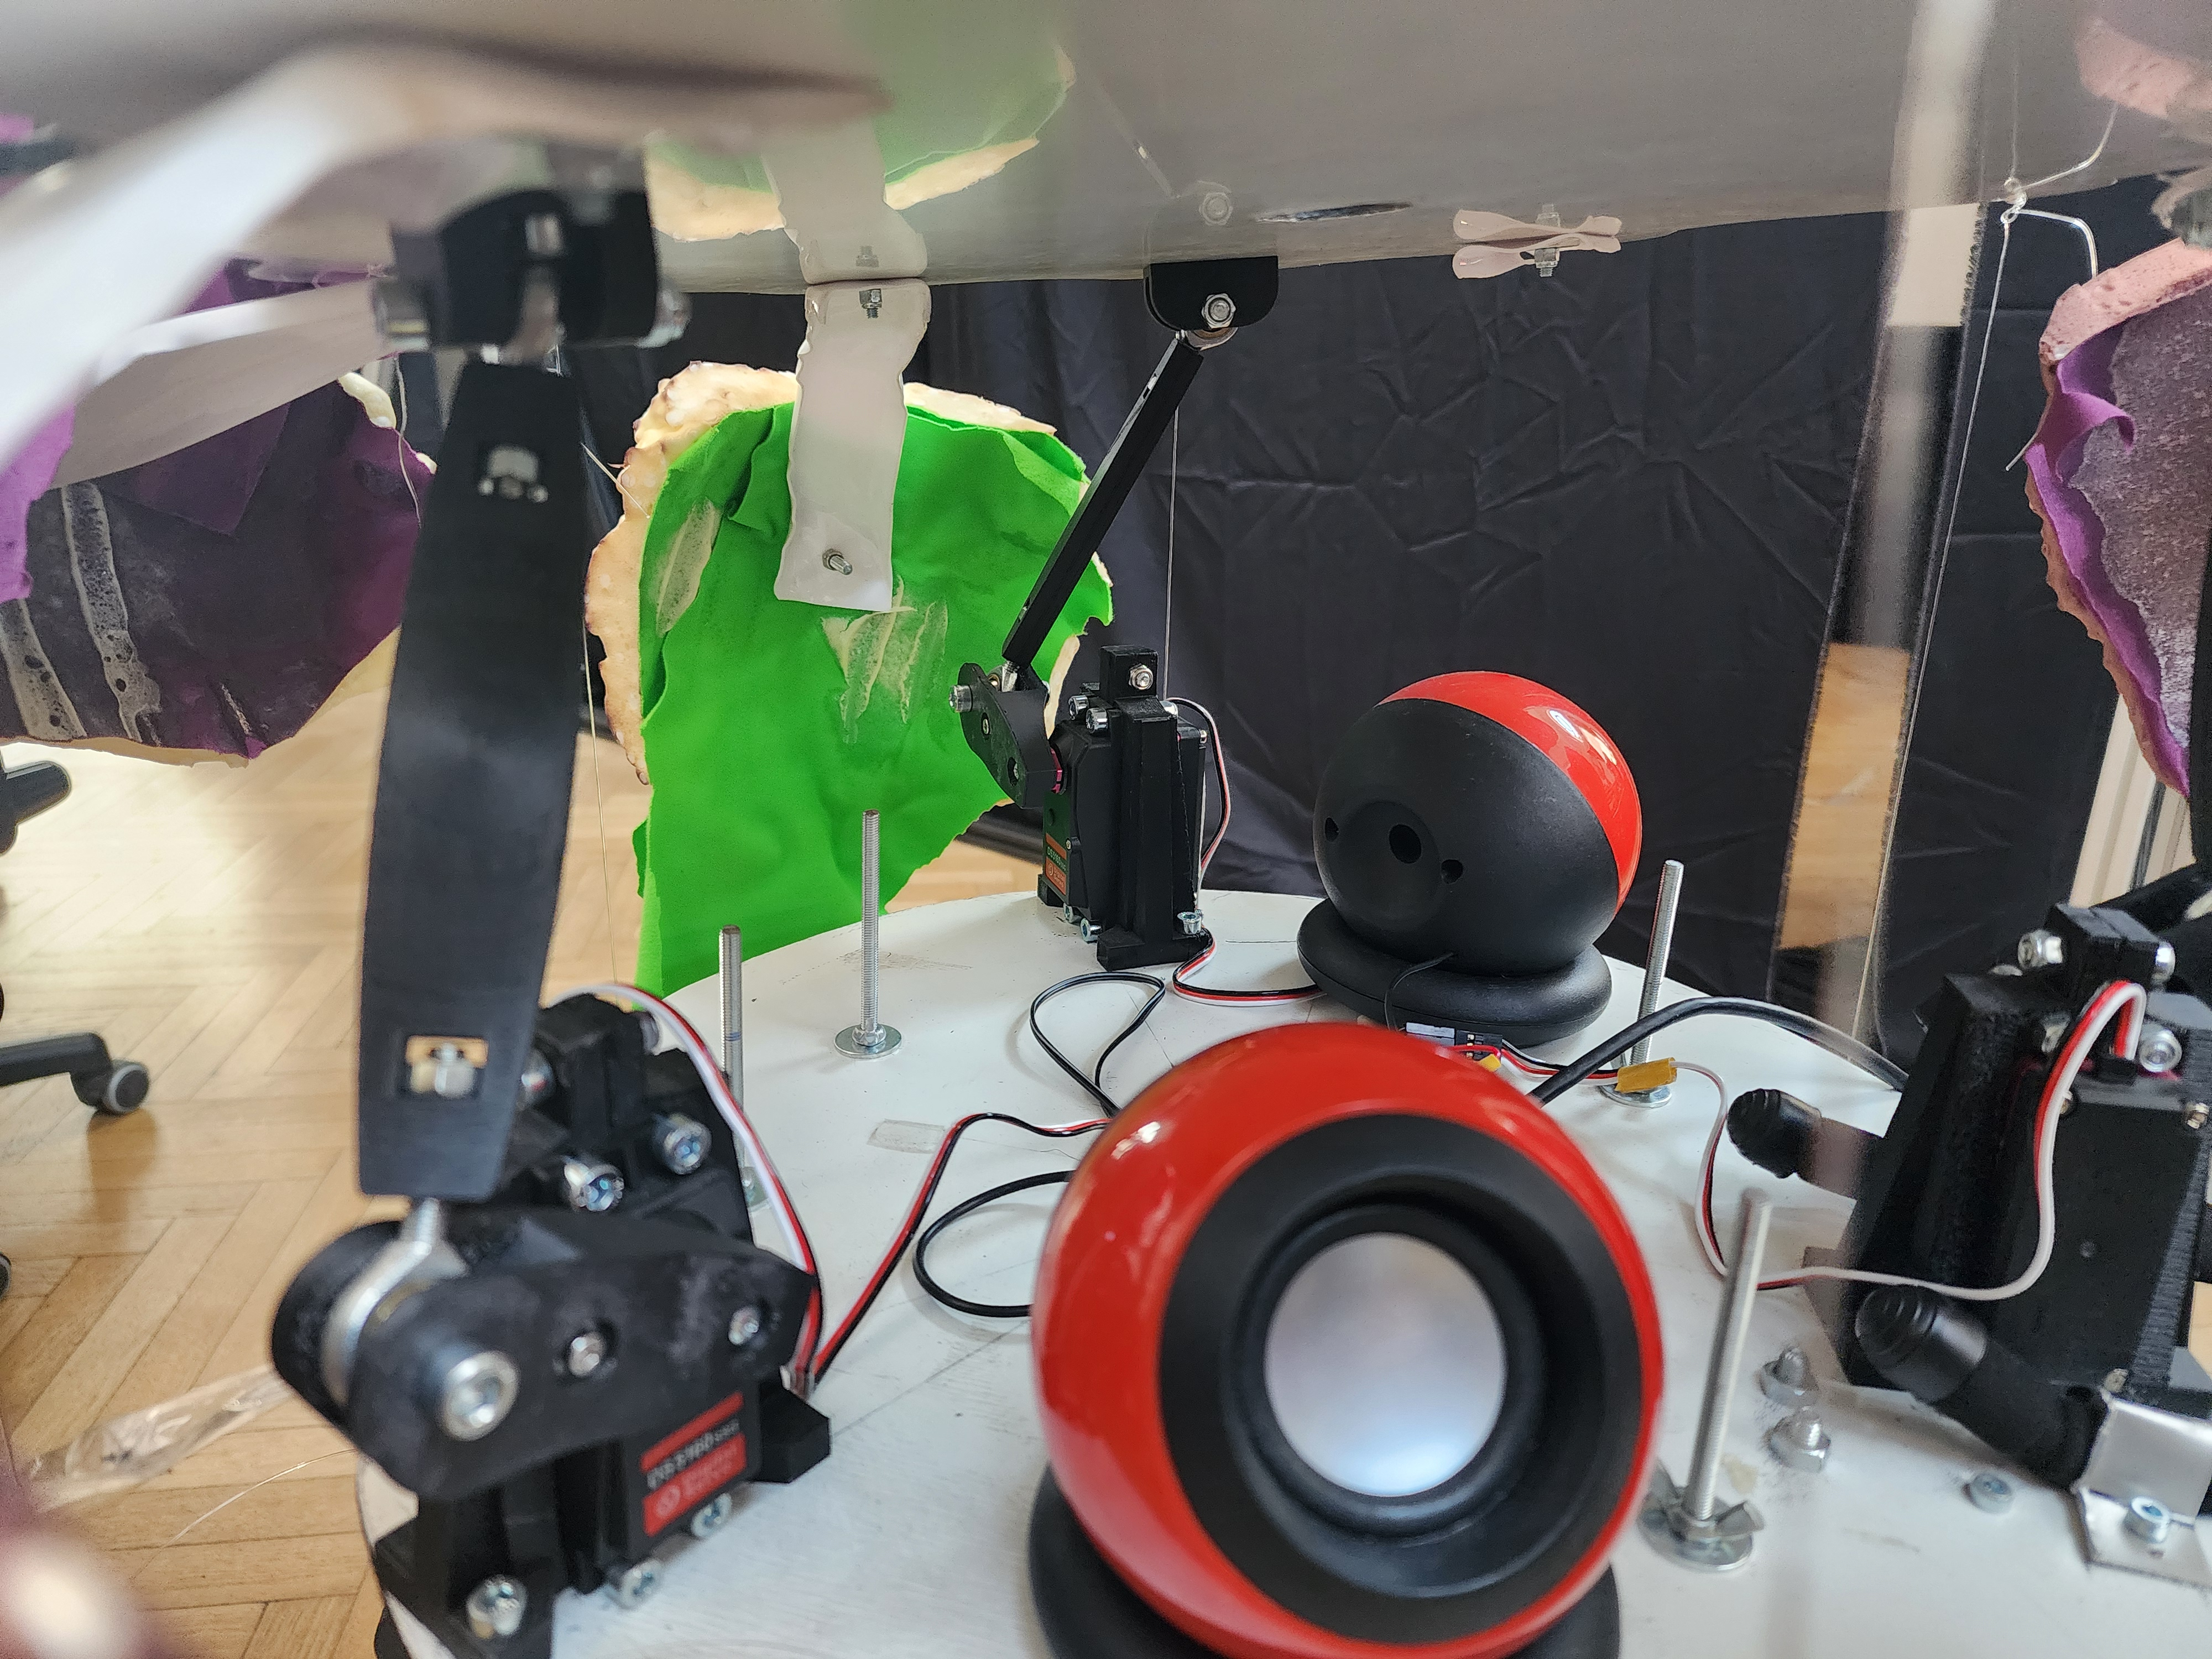
\includegraphics[width=\textwidth]{Images/NewHeadDoubleJoint (6).jpg}
        \caption{Head Arm with Rod Ends (Sway to right)}
        \label{fig:head_arm_rod_end_right}
    \end{minipage}
    \hfill
    \begin{minipage}{0.45\textwidth}
        \centering
        \includegraphics[width=\textwidth]{Images/NewHeadDoubleJoint (2).jpg}
        \caption{Head Arm with Rod Ends (Sway to left)}
        \label{fig:head_arm_rod_end_left}
    \end{minipage}
\end{figure}

The final implementation combines 3D printed structural components with metal heim joints to achieve optimal balance between cost, performance, and maintainability. Load capacity testing validates the enhanced design's capability to handle operational loads without component failure, with longevity testing demonstrating sustained performance under extended operational scenarios typical of social robot research applications. This reliable head control mechanism provided the stable platform necessary for sophisticated camera integration detailed in the subsequent section.

% REORG_TAG: moved here from Camera Integration and Mounting Solutions
\subsection{Camera Integration and Mounting}

The integration of the Oak-D Pro camera within Tino's soft fabric structure presented unique challenges requiring stable mechanical mounting while maintaining the robot's aesthetic characteristics and preventing the camera from becoming a prominent visual feature. The original Raspberry Pi camera mount exhibited excessive flexibility and vibration issues that compromised image quality, necessitating a complete redesign approach that balanced stability, concealment, and operational requirements.

\subsubsection{Tripod Mounting System and Structural Integration}

The camera mounting solution utilizes a tripod-based support system with simple brackets to create fixed and stable camera support that eliminates flexibility and vibration issues. The tripod mounting system provides significant improvement in camera positioning stability compared to the flexible original mount, with static deflection testing validating adequate stiffness for high-quality image acquisition during movement. The camera mounting system operates independently from the Stewart platform head mechanism, providing dedicated stable positioning for the Oak-D Pro camera without mechanical coupling to head movements.

\begin{figure}[H]
    \centering
    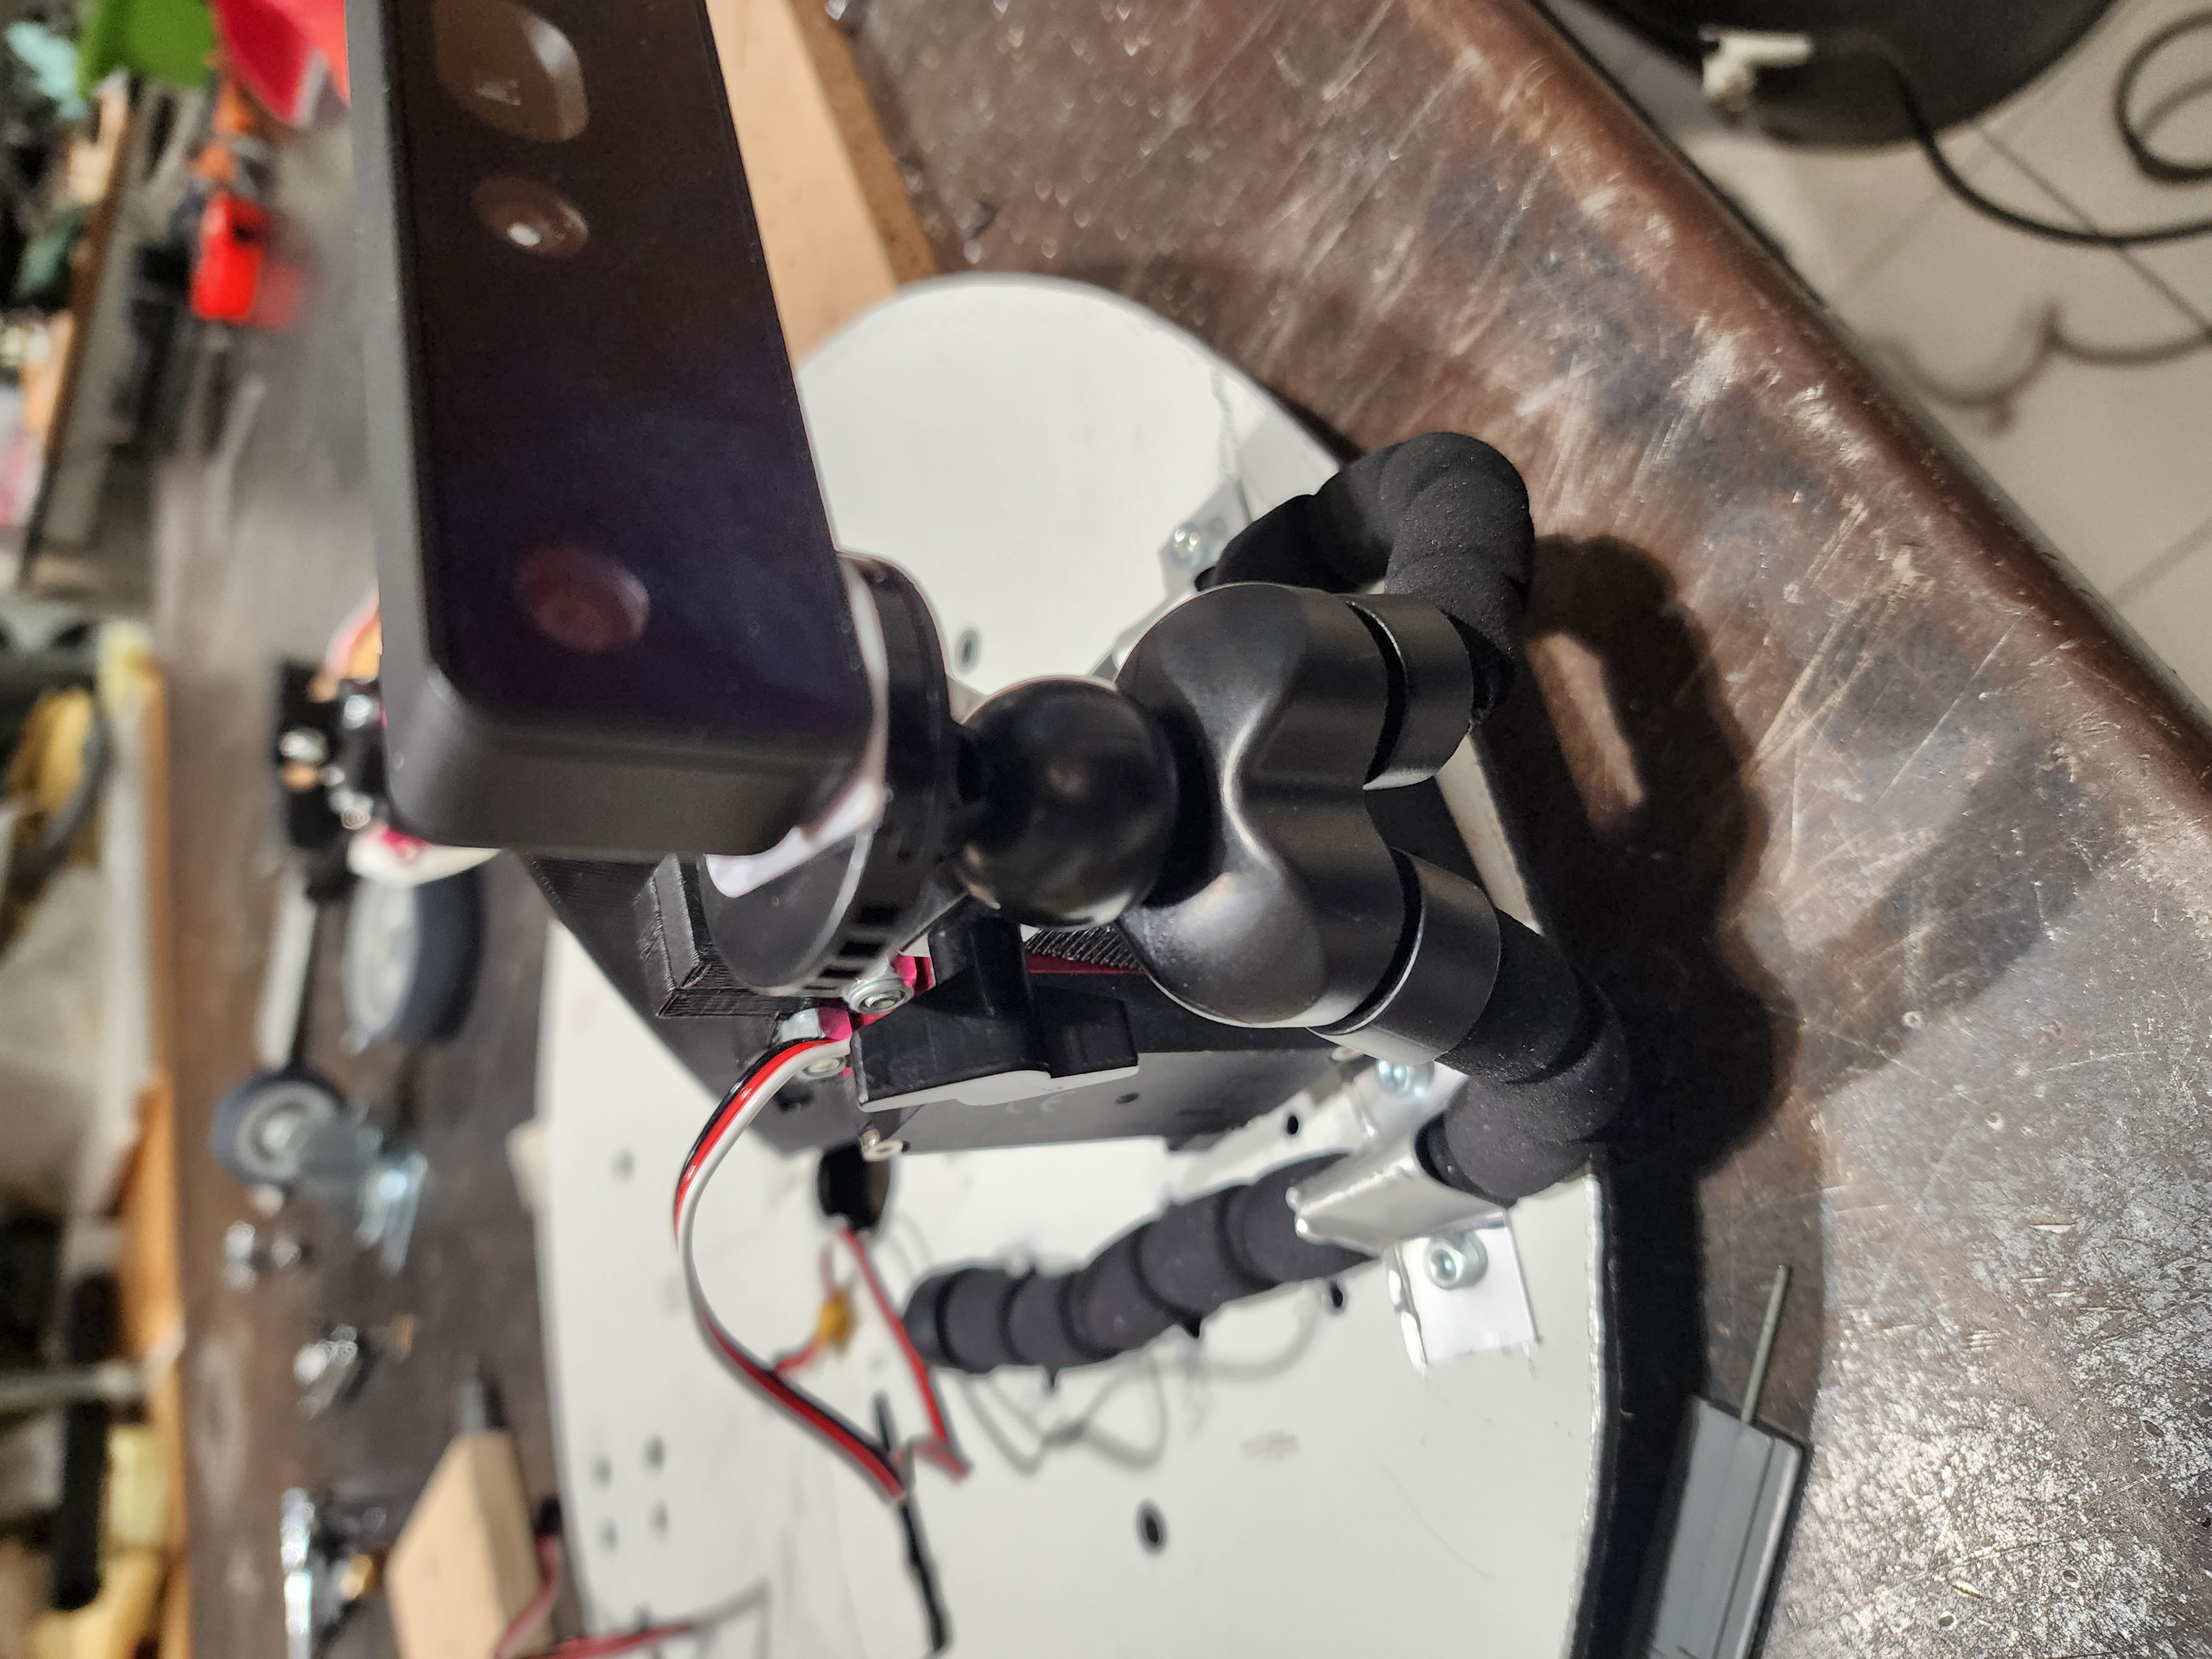
\includegraphics[width=0.6\textwidth, angle=-90]{Images/TripodOnHeadCamera.jpg}
    \caption{Oak-D Pro Camera Mounted on Tripod System}
    \label{fig:tripod_camera_mount}
\end{figure}

The mounting system accommodates the existing servo head geometry while providing secure attachment points for the Oak-D Pro camera, with geometric constraints requiring custom bracket design that works within available space while providing adequate support. Mechanical interfaces utilize standard mounting hardware enabling camera removal for maintenance without requiring bracket system modification.

\begin{figure}[H]
    \centering
    \begin{minipage}{0.45\textwidth}
        \centering
        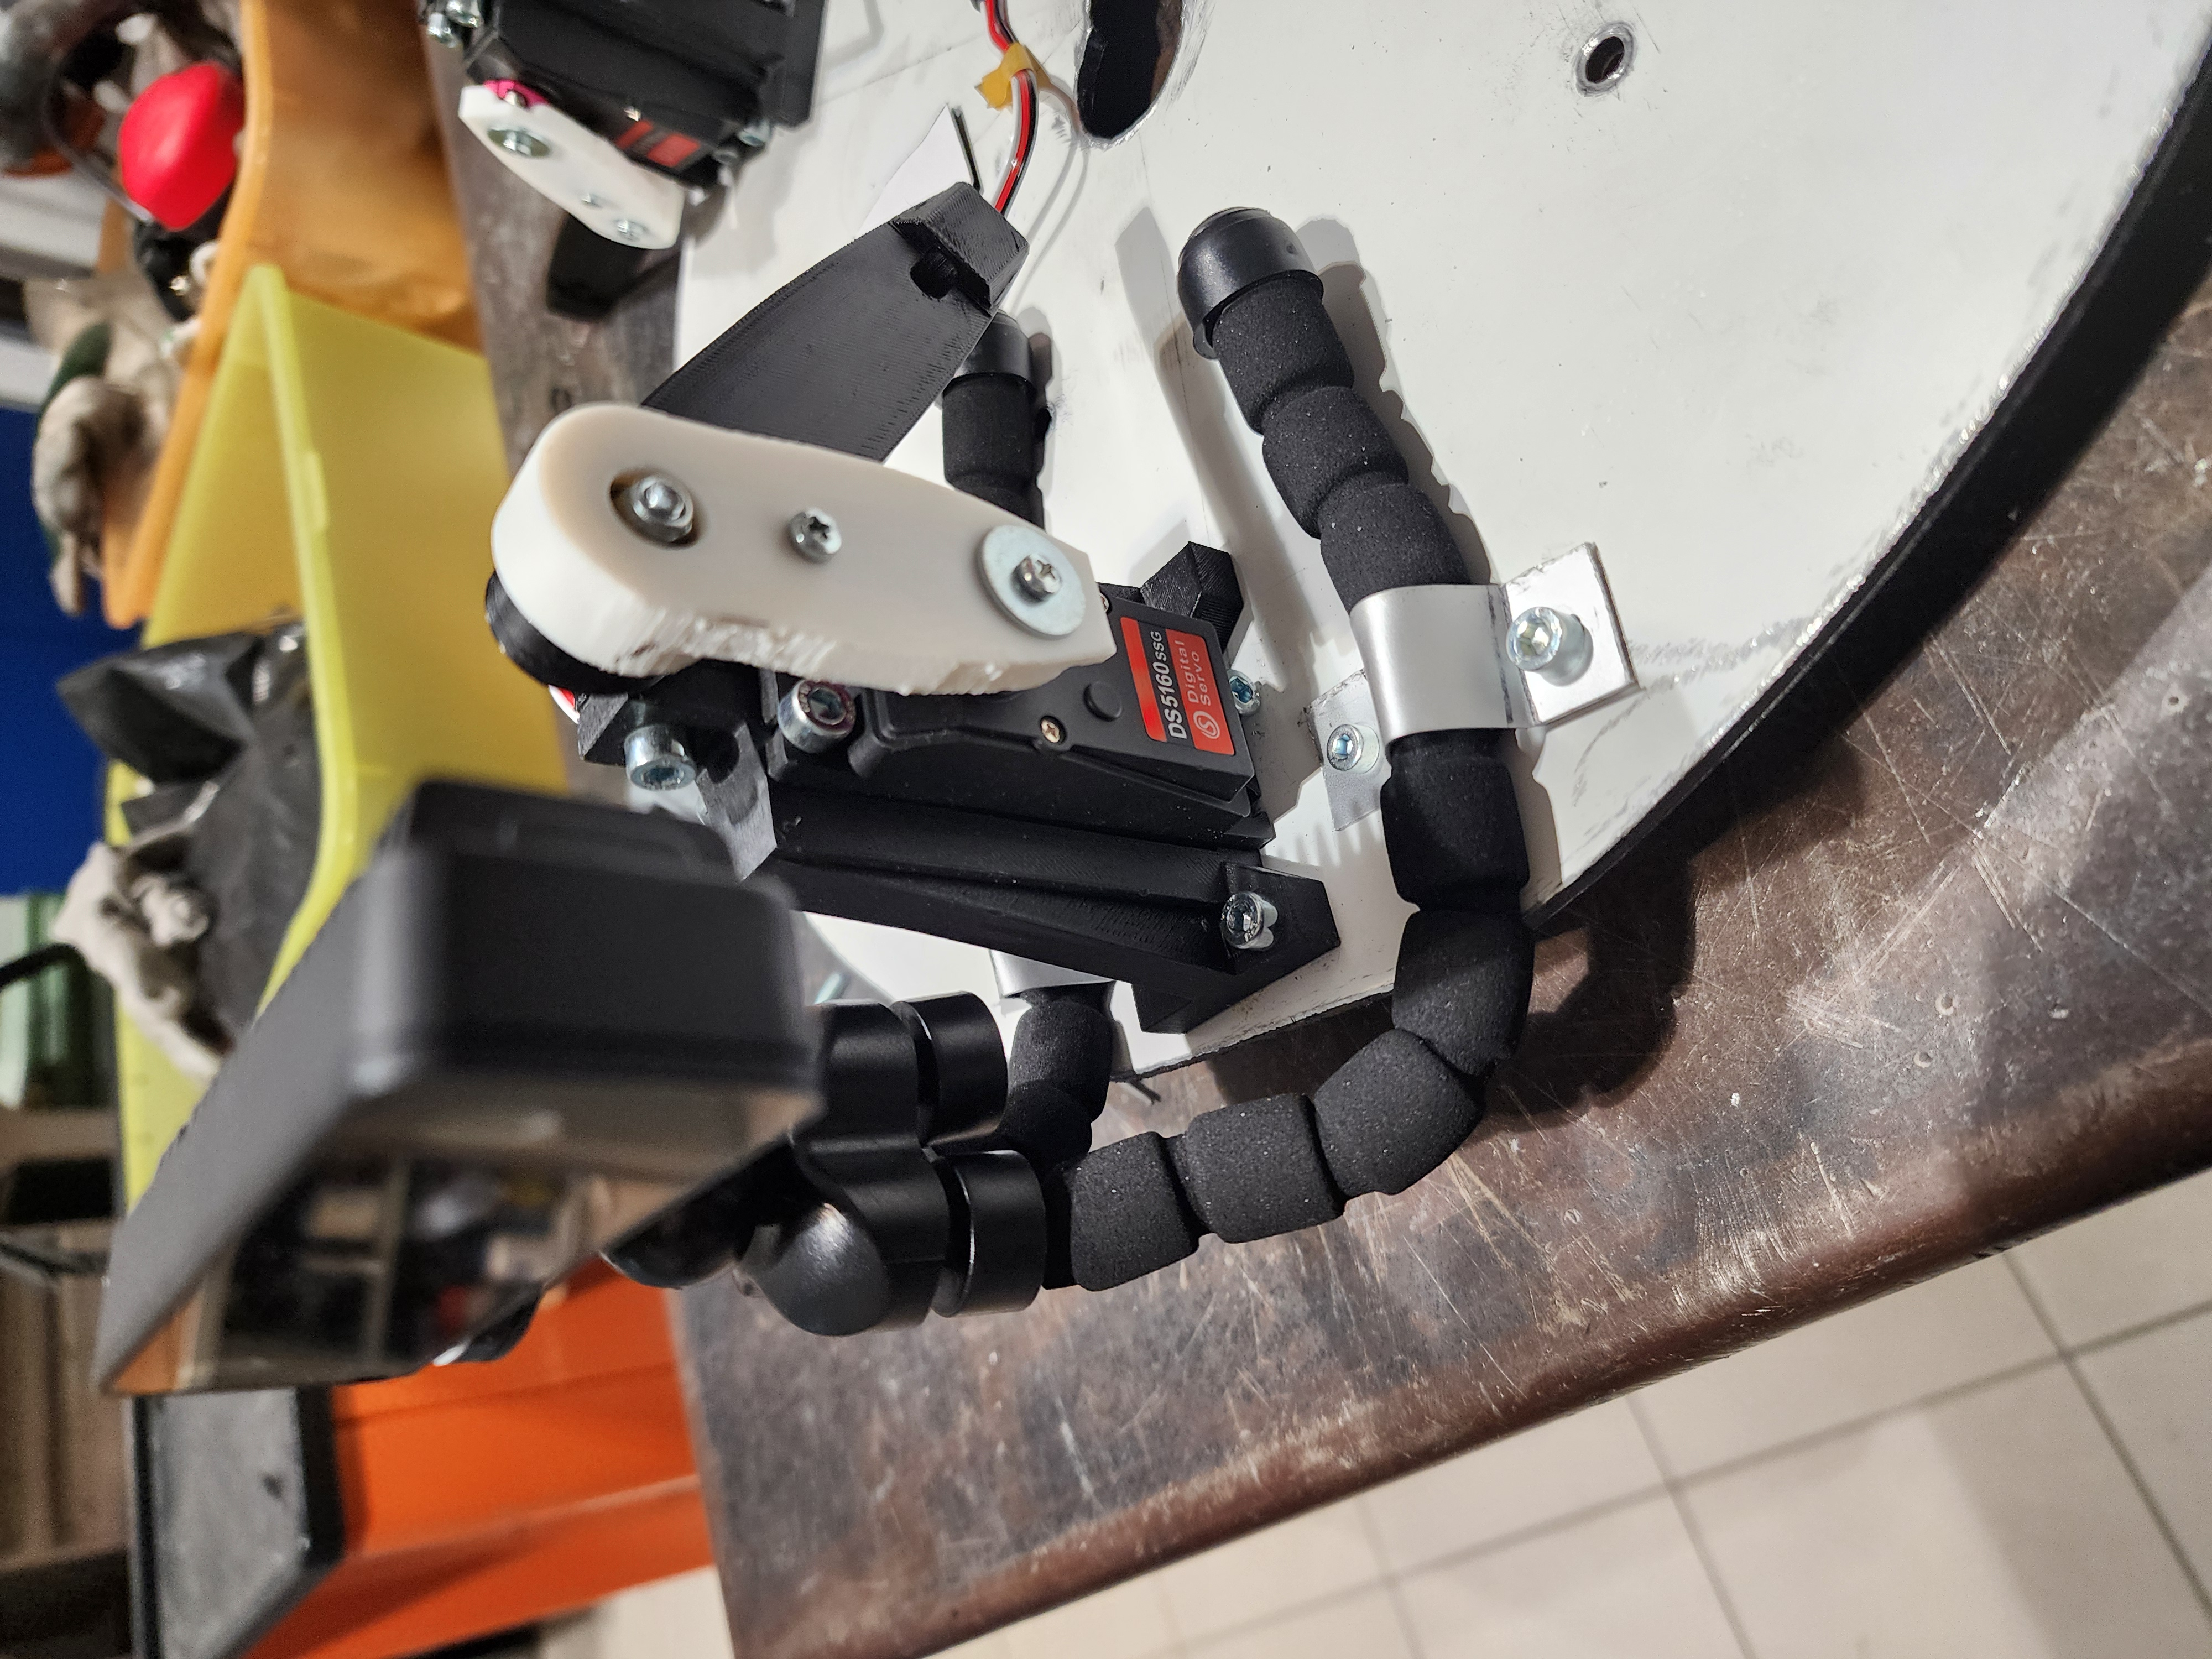
\includegraphics[width=\textwidth, angle=-90]{Images/TripodOnHeadCamera (3).jpg}
        \caption{Oak-D Pro Camera Mounted on Tripod System (Side View)}
        \label{fig:tripod_camera_mount_side}
    \end{minipage}
    \hfill
    \begin{minipage}{0.45\textwidth}
        \centering
        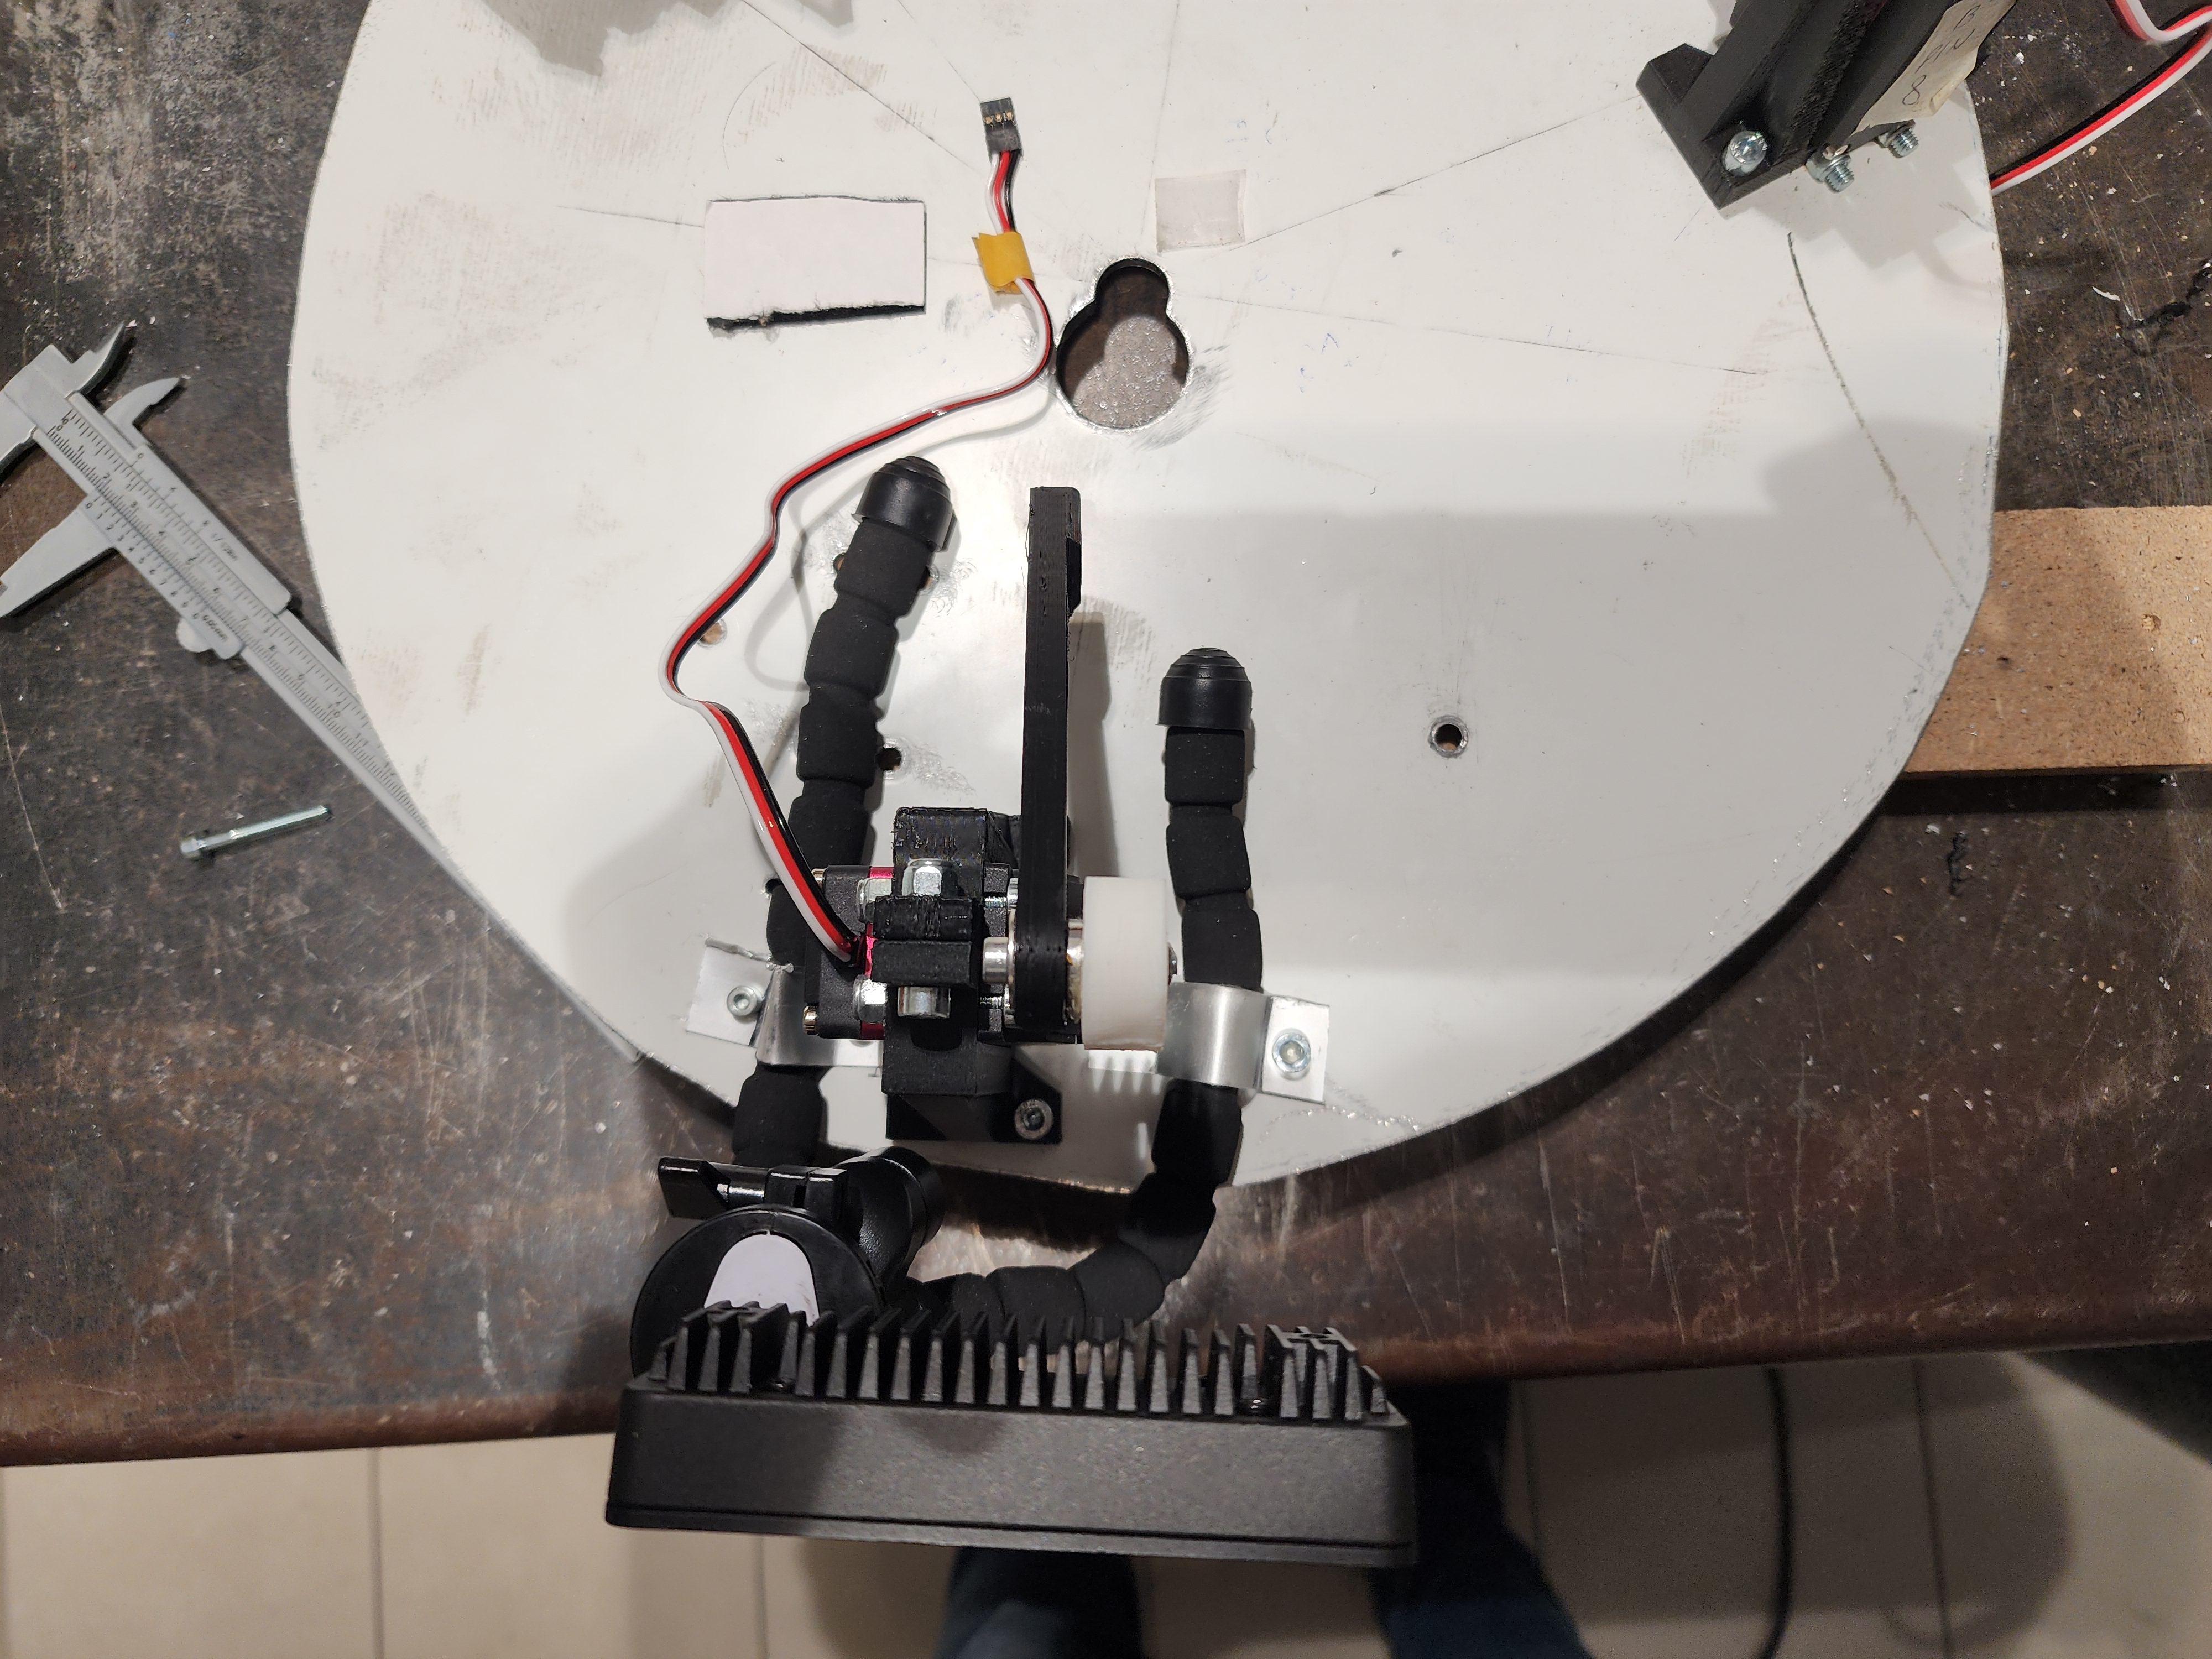
\includegraphics[width=\textwidth]{Images/TripodOnHeadCamera (2).jpg}
        \caption{Oak-D Pro Camera Mounted on Tripod System (Top View)}
        \label{fig:tripod_camera_mount_top}
    \end{minipage}
\end{figure}

\subsubsection{Fabric Integration and Camera Concealment System}

The fabric integration challenge required maintaining camera visibility while preserving Tino's fabric aesthetic and protecting sensitive camera components. Fabric positioning strategies prevent interference with camera sensing through velcro attachment systems that provide secure fabric positioning, preventing fabric drift into camera field of view during operational periods. Testing procedures validate fabric positioning effectiveness under various operational scenarios including head movement, robot locomotion, and extended operational periods.

\begin{figure}[H]
    \centering
    \begin{minipage}{0.45\textwidth}
        \centering
        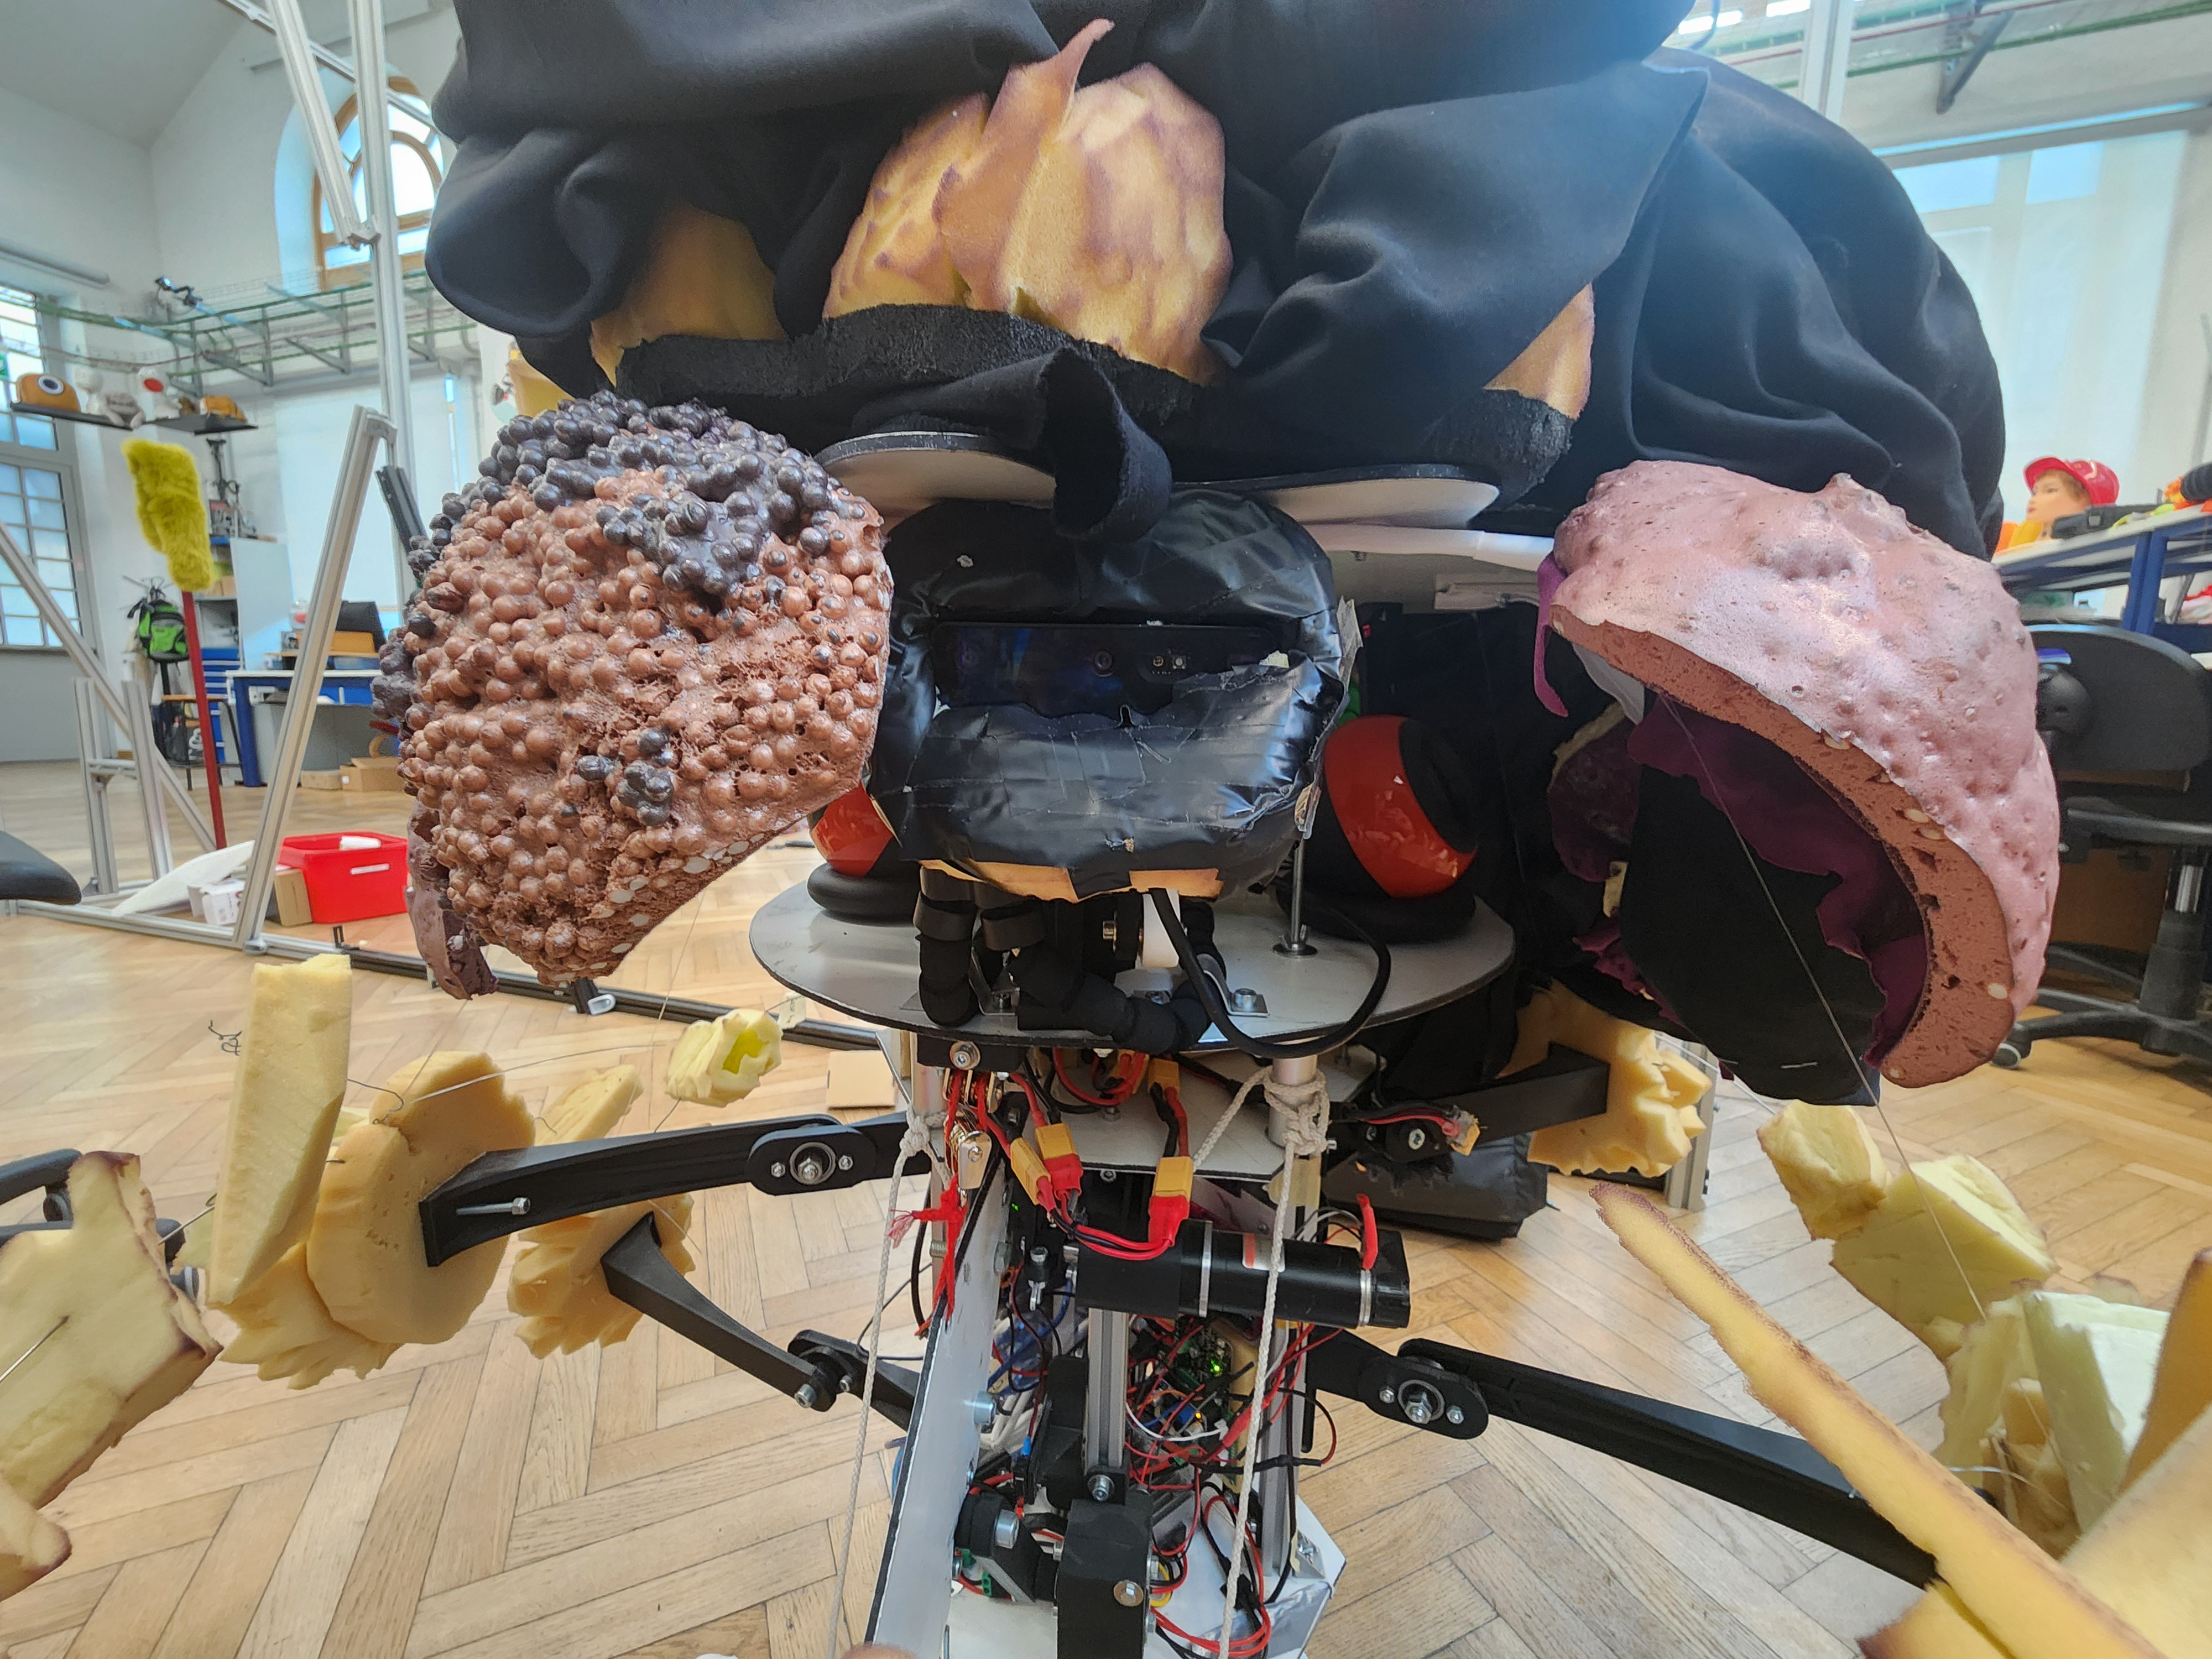
\includegraphics[width=\textwidth]{Images/FirstTryCameraHiding.jpg}
        \caption{Initial Camera Concealment Attempt (Front View)}
        \label{fig:first_try_camera_hiding}
    \end{minipage}
    \hfill
    \begin{minipage}{0.45\textwidth}
        \centering
        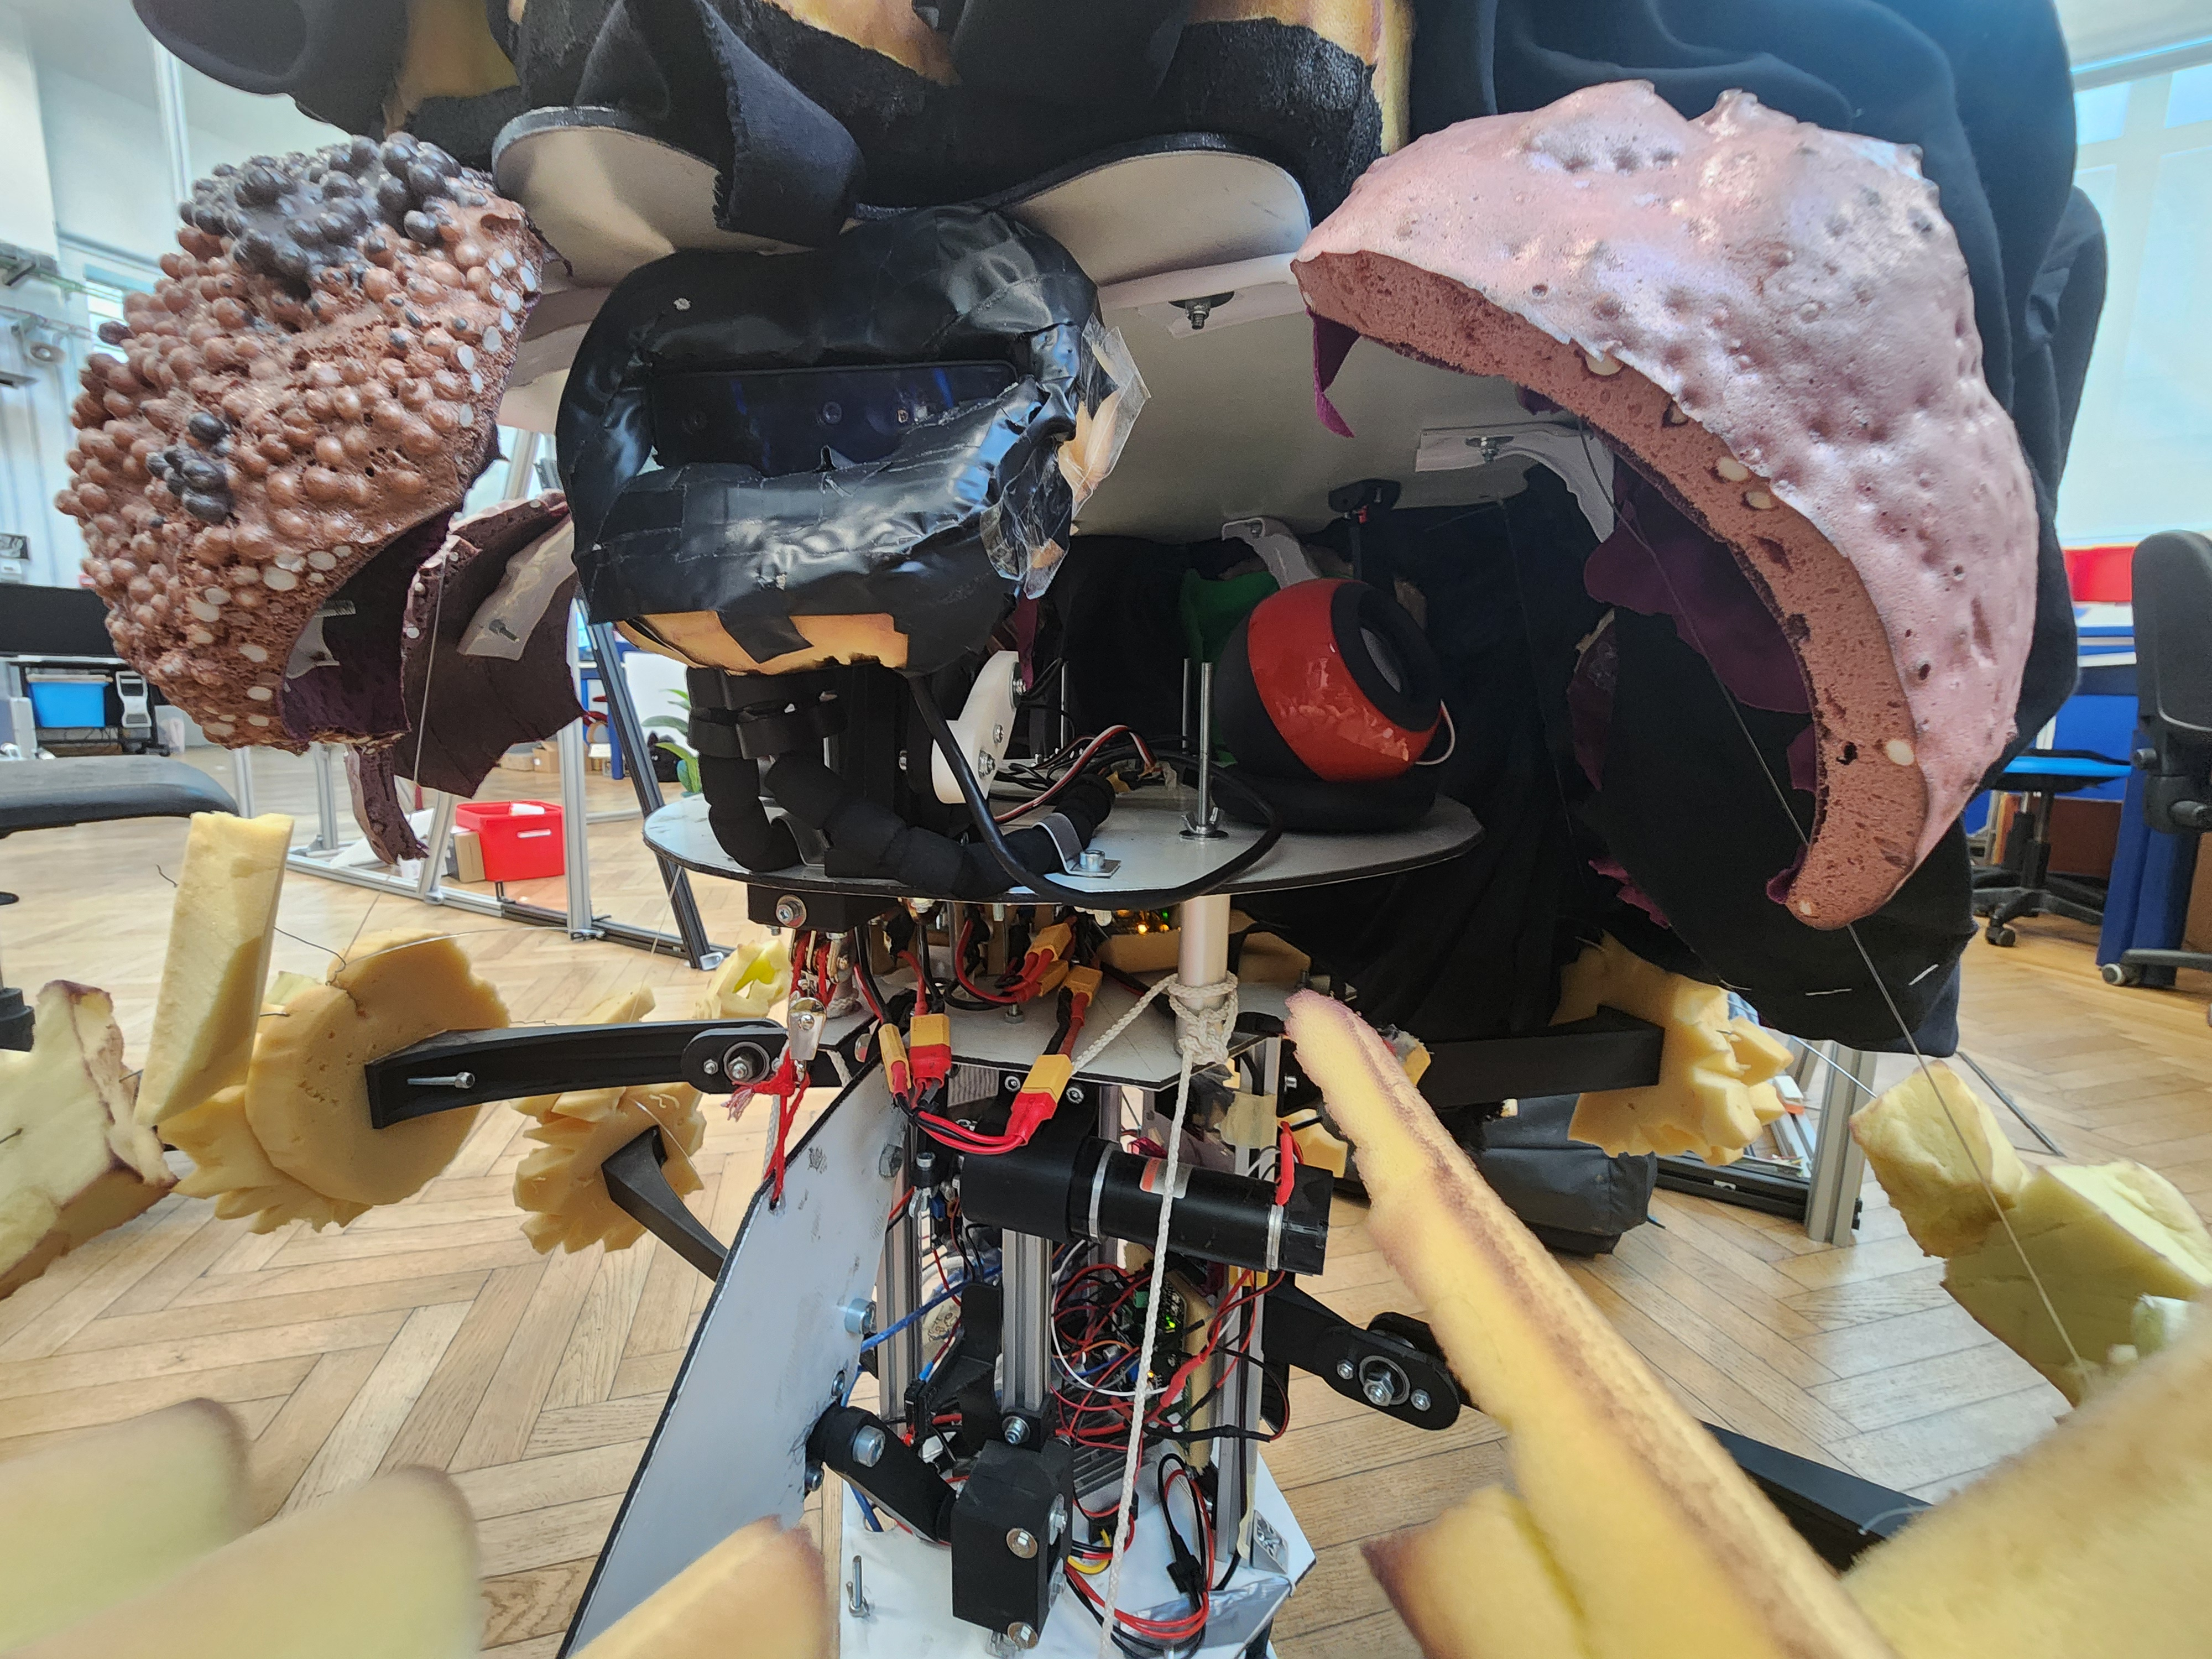
\includegraphics[width=\textwidth]{Images/FirstTryCameraHiding (3).jpg}
        \caption{Initial Camera Concealment Attempt (Side View)}
        \label{fig:camera_hiding_mesh}
    \end{minipage}
\end{figure}

The comprehensive camera shell system provides protection and fabric integration while maintaining optimal camera performance and heat dissipation characteristics. The custom shell design provides camera protection through strategic ventilation openings that enable heat dissipation without compromising environmental protection, with shell geometry optimizing airflow characteristics while minimizing dust ingress.

\begin{figure}[H]
    \centering
    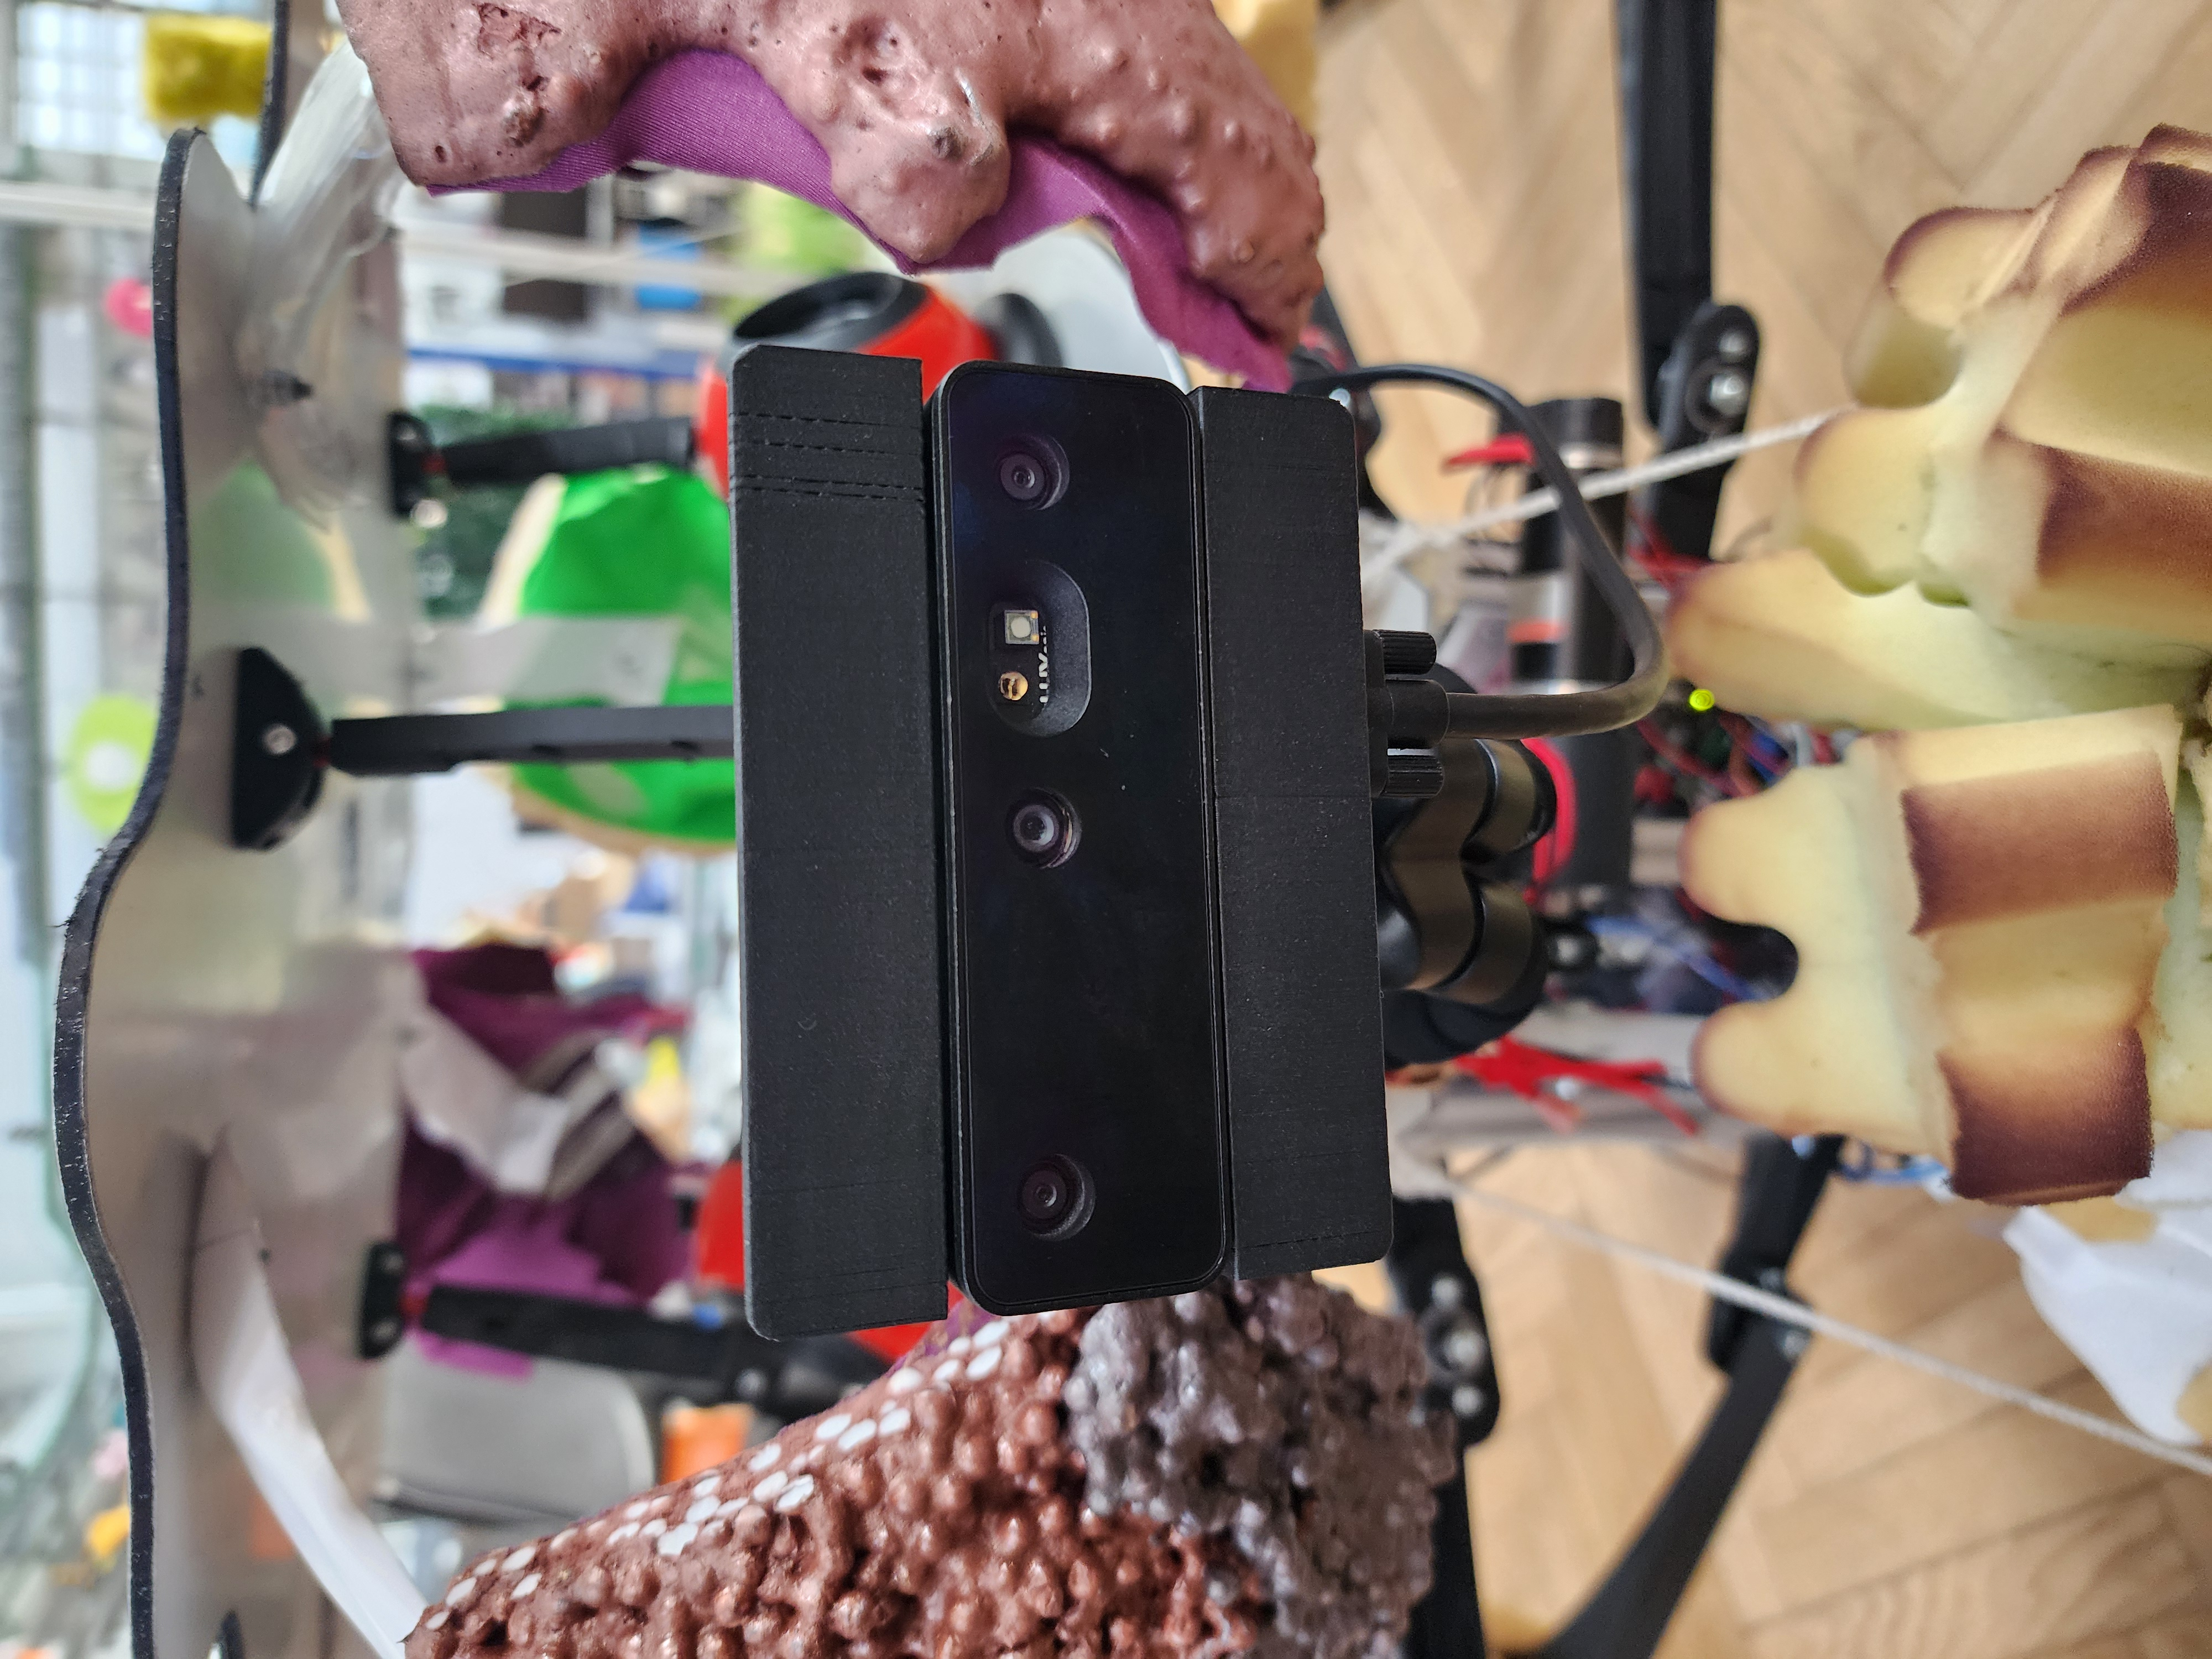
\includegraphics[height=8cm, angle=-90]{Images/CameraCasingNoMesh.jpg}
    \caption{Camera Casing without Mesh Covering}
    \label{fig:camera_casing_no_mesh}
\end{figure}

Attachment integration with the tripod mounting system provides secure shell mounting that enables camera access for maintenance while providing operational protection. Thermal management considerations ensure adequate heat dissipation during extended operation periods, particularly during high-resolution stereo processing that generates significant thermal loads.

\begin{figure}[H]
    \centering
    \begin{minipage}{0.45\textwidth}
        \centering
        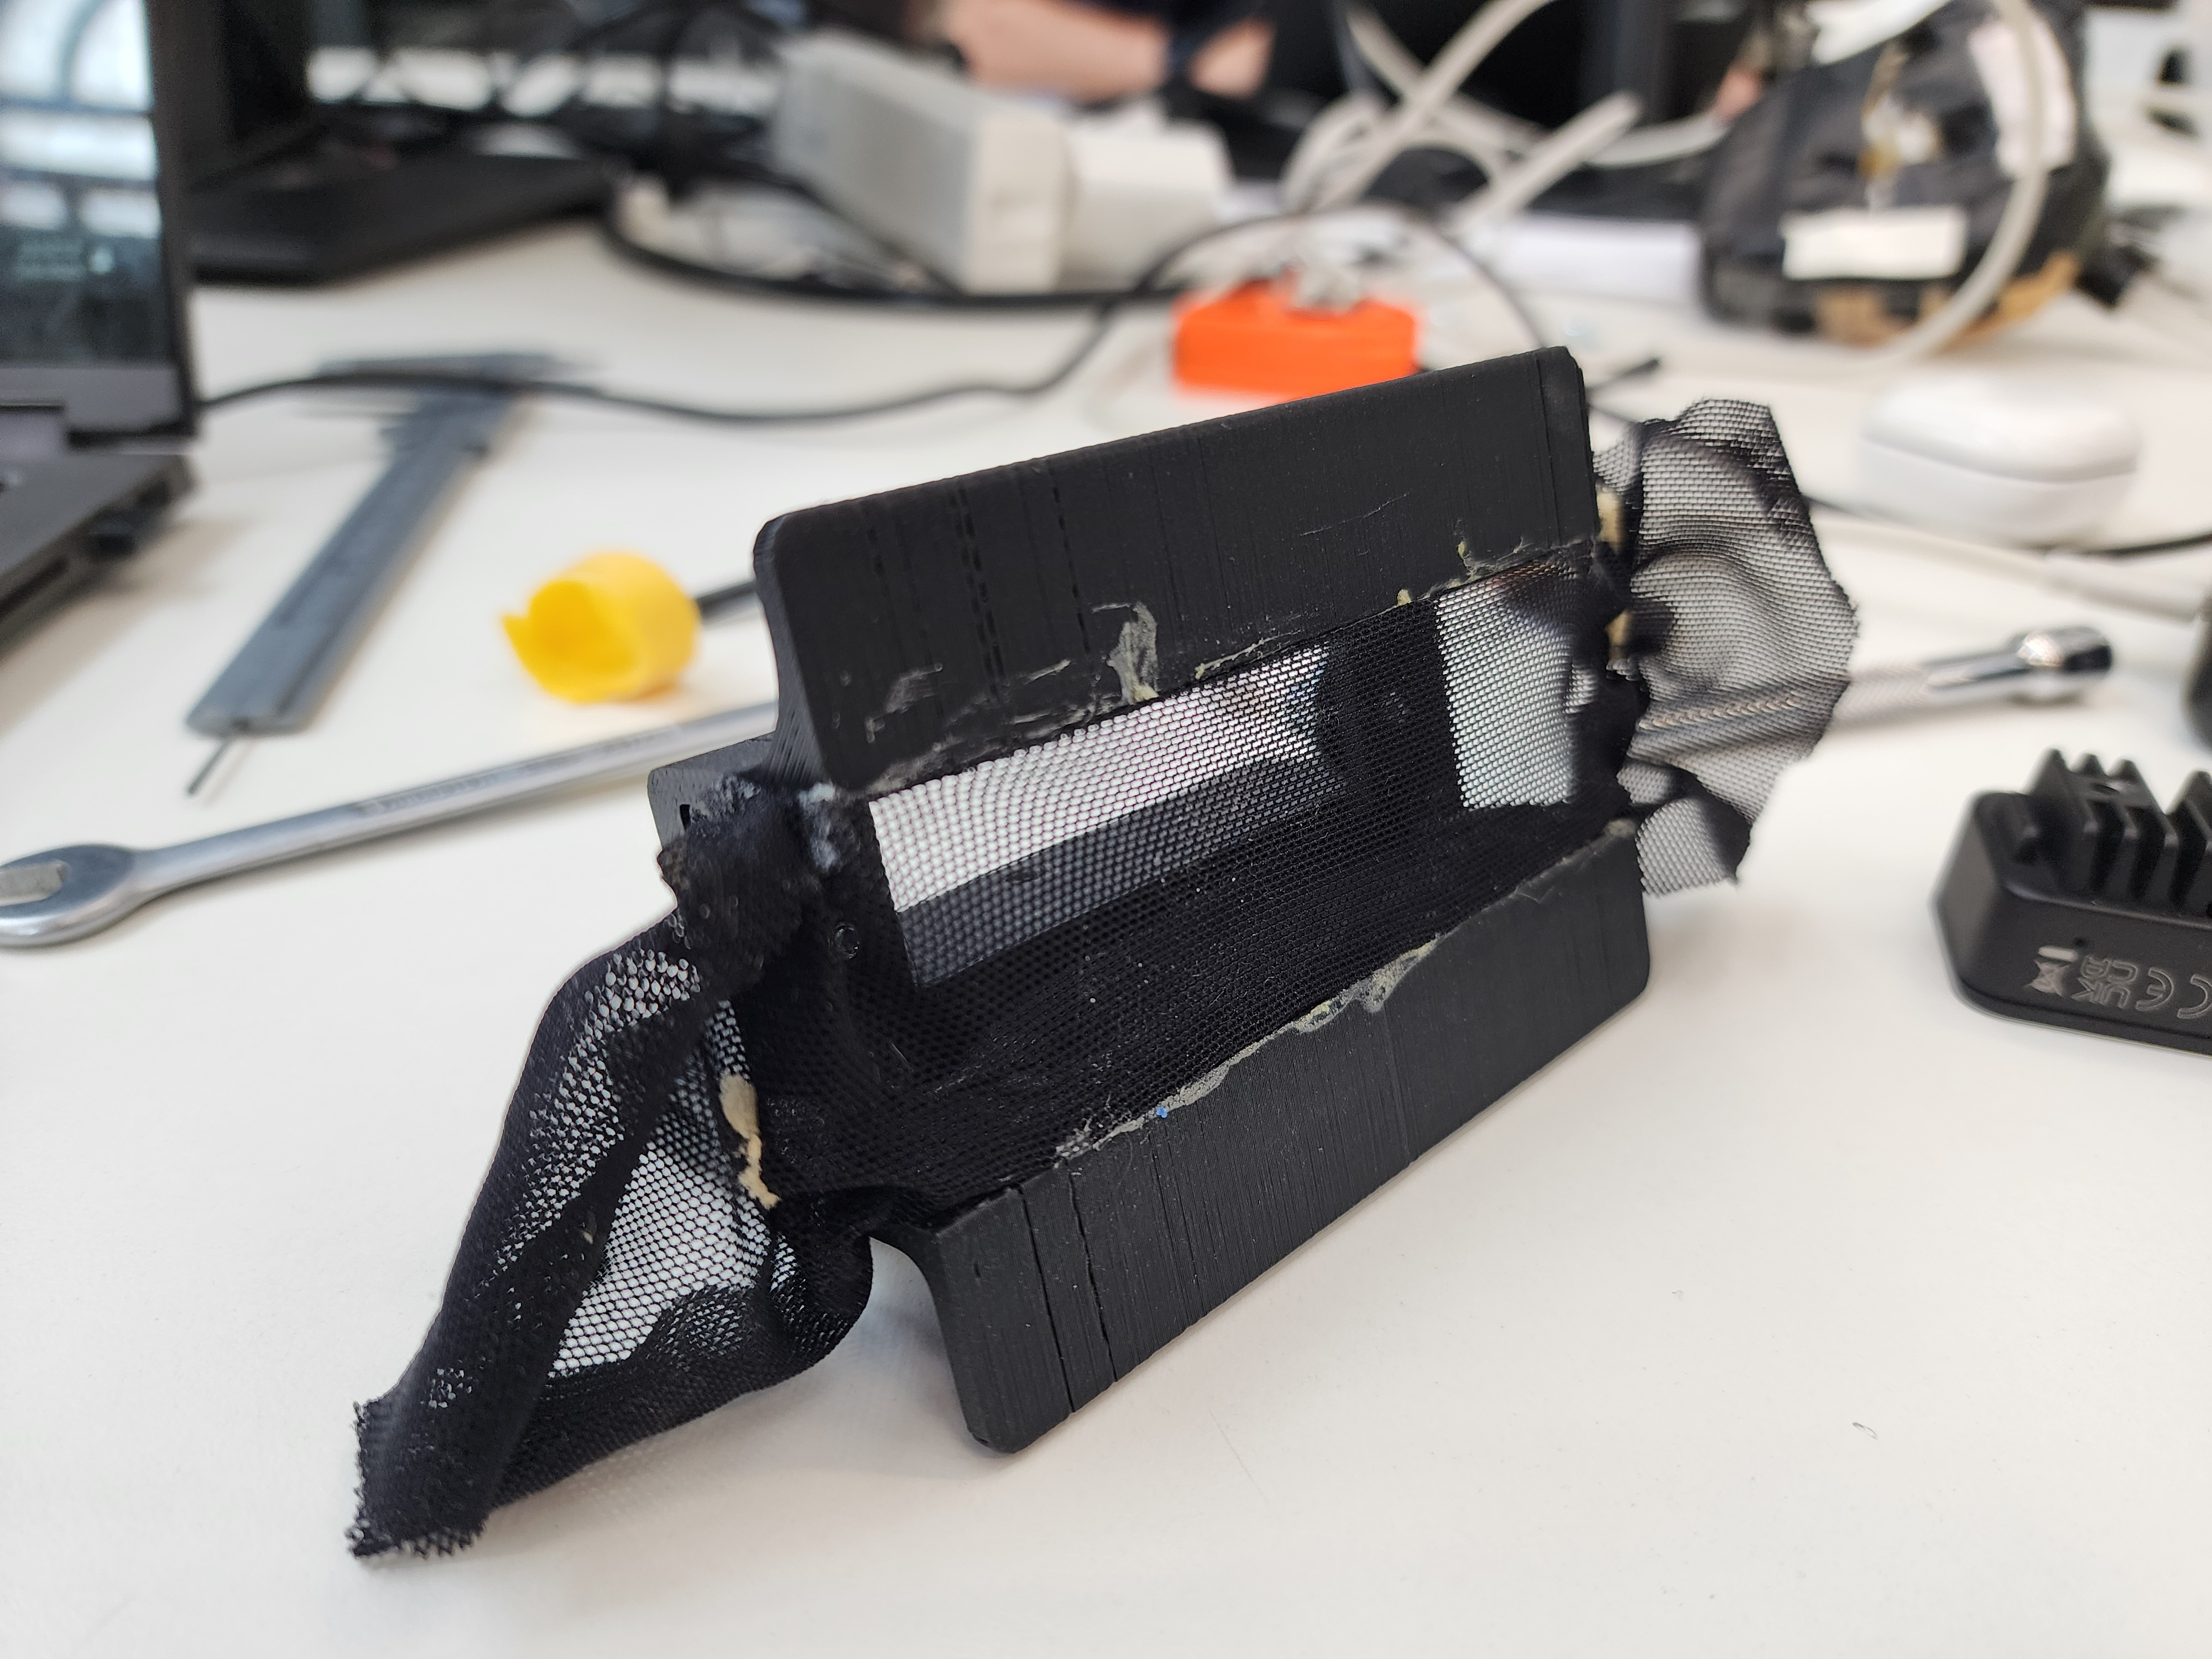
\includegraphics[width=0.8\textwidth]{Images/CameraCasingMesh.jpg}
        \caption{Camera Casing with Mesh Covering (No camera)} 
        \label{fig:camera_casing_mesh}
    \end{minipage}
    \hfill
    \begin{minipage}{0.45\textwidth}
        \centering
        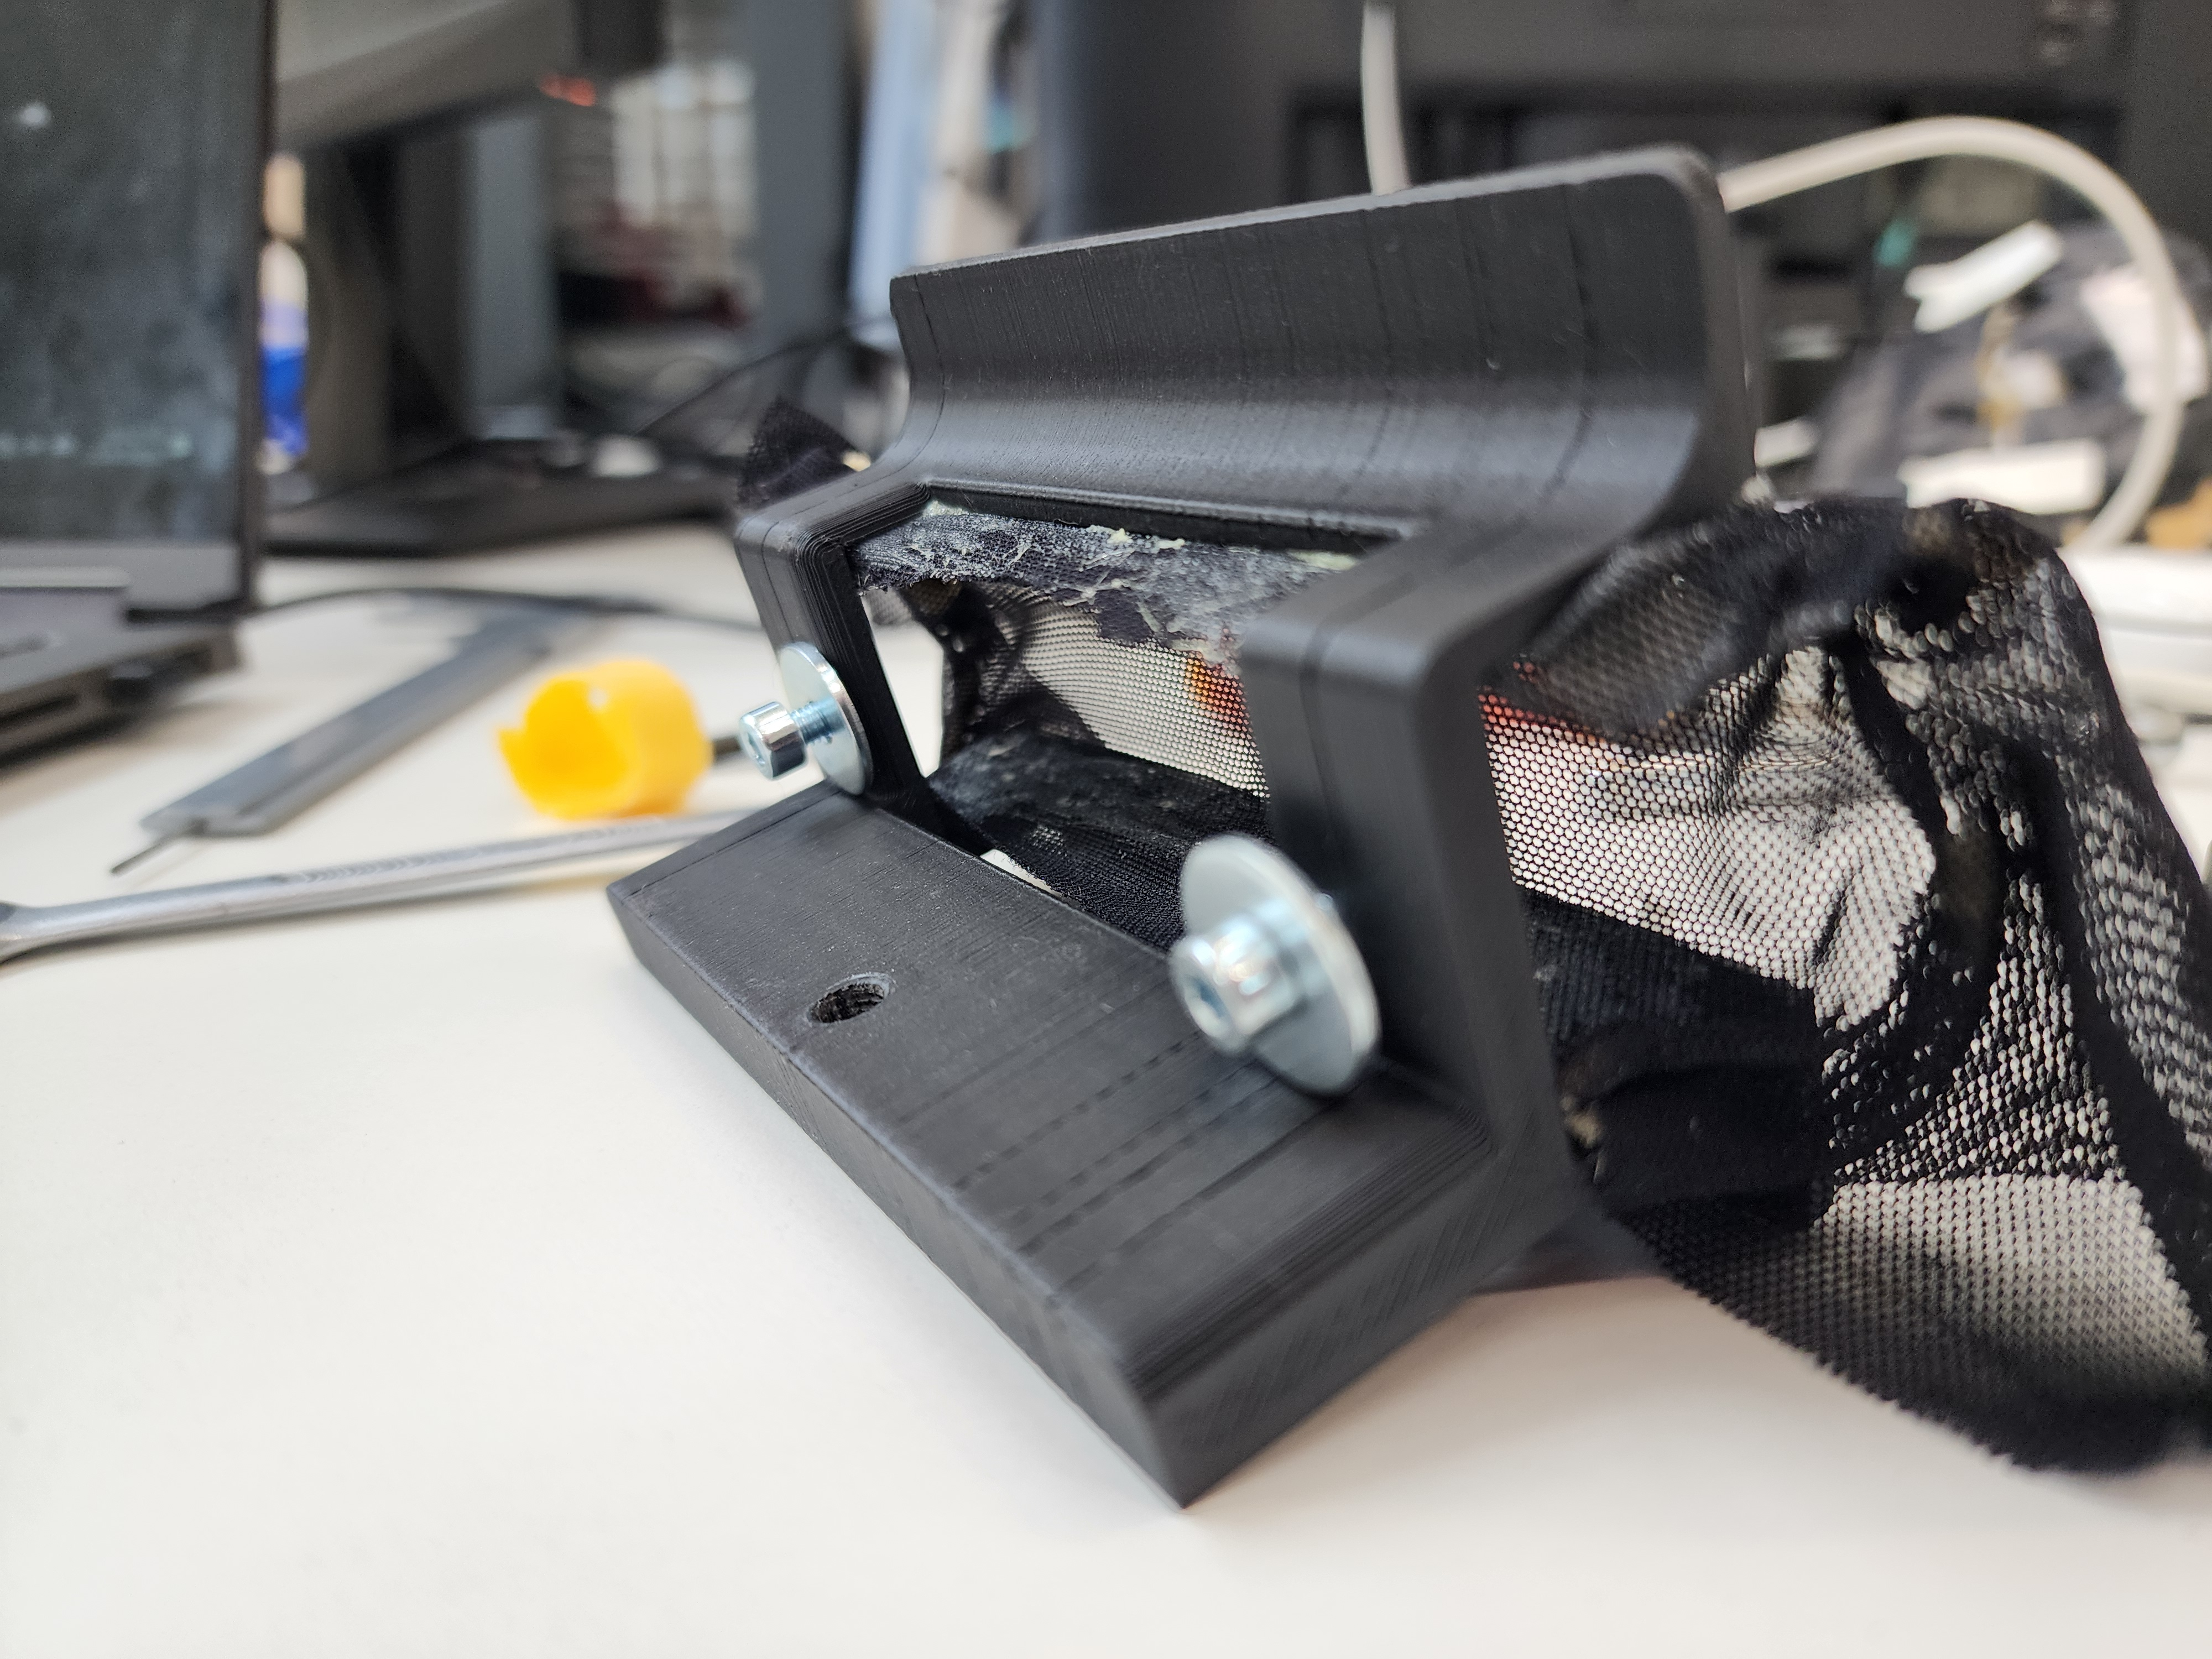
\includegraphics[width=0.8\textwidth]{Images/CameraCasingMesh (2).jpg}
        \caption{Camera Casing with Mesh Covering (No camera)}
        \label{fig:camera_casing_mesh_back}
    \end{minipage}
\end{figure}

The fabric control system utilizes velcro attachments integrated with shell flaps to provide positive fabric positioning control, with velcro implementation including both shell-mounted components and fabric-sewn counterparts that provide reliable attachment while enabling fabric removal for maintenance. Mesh covering implementation conceals camera presence from casual observation while maintaining full optical transmission characteristics, with optical testing validating maintained image quality and depth sensing performance through the concealment system.

\begin{figure}[H]
    \centering
    \begin{minipage}{0.45\textwidth}
        \centering
        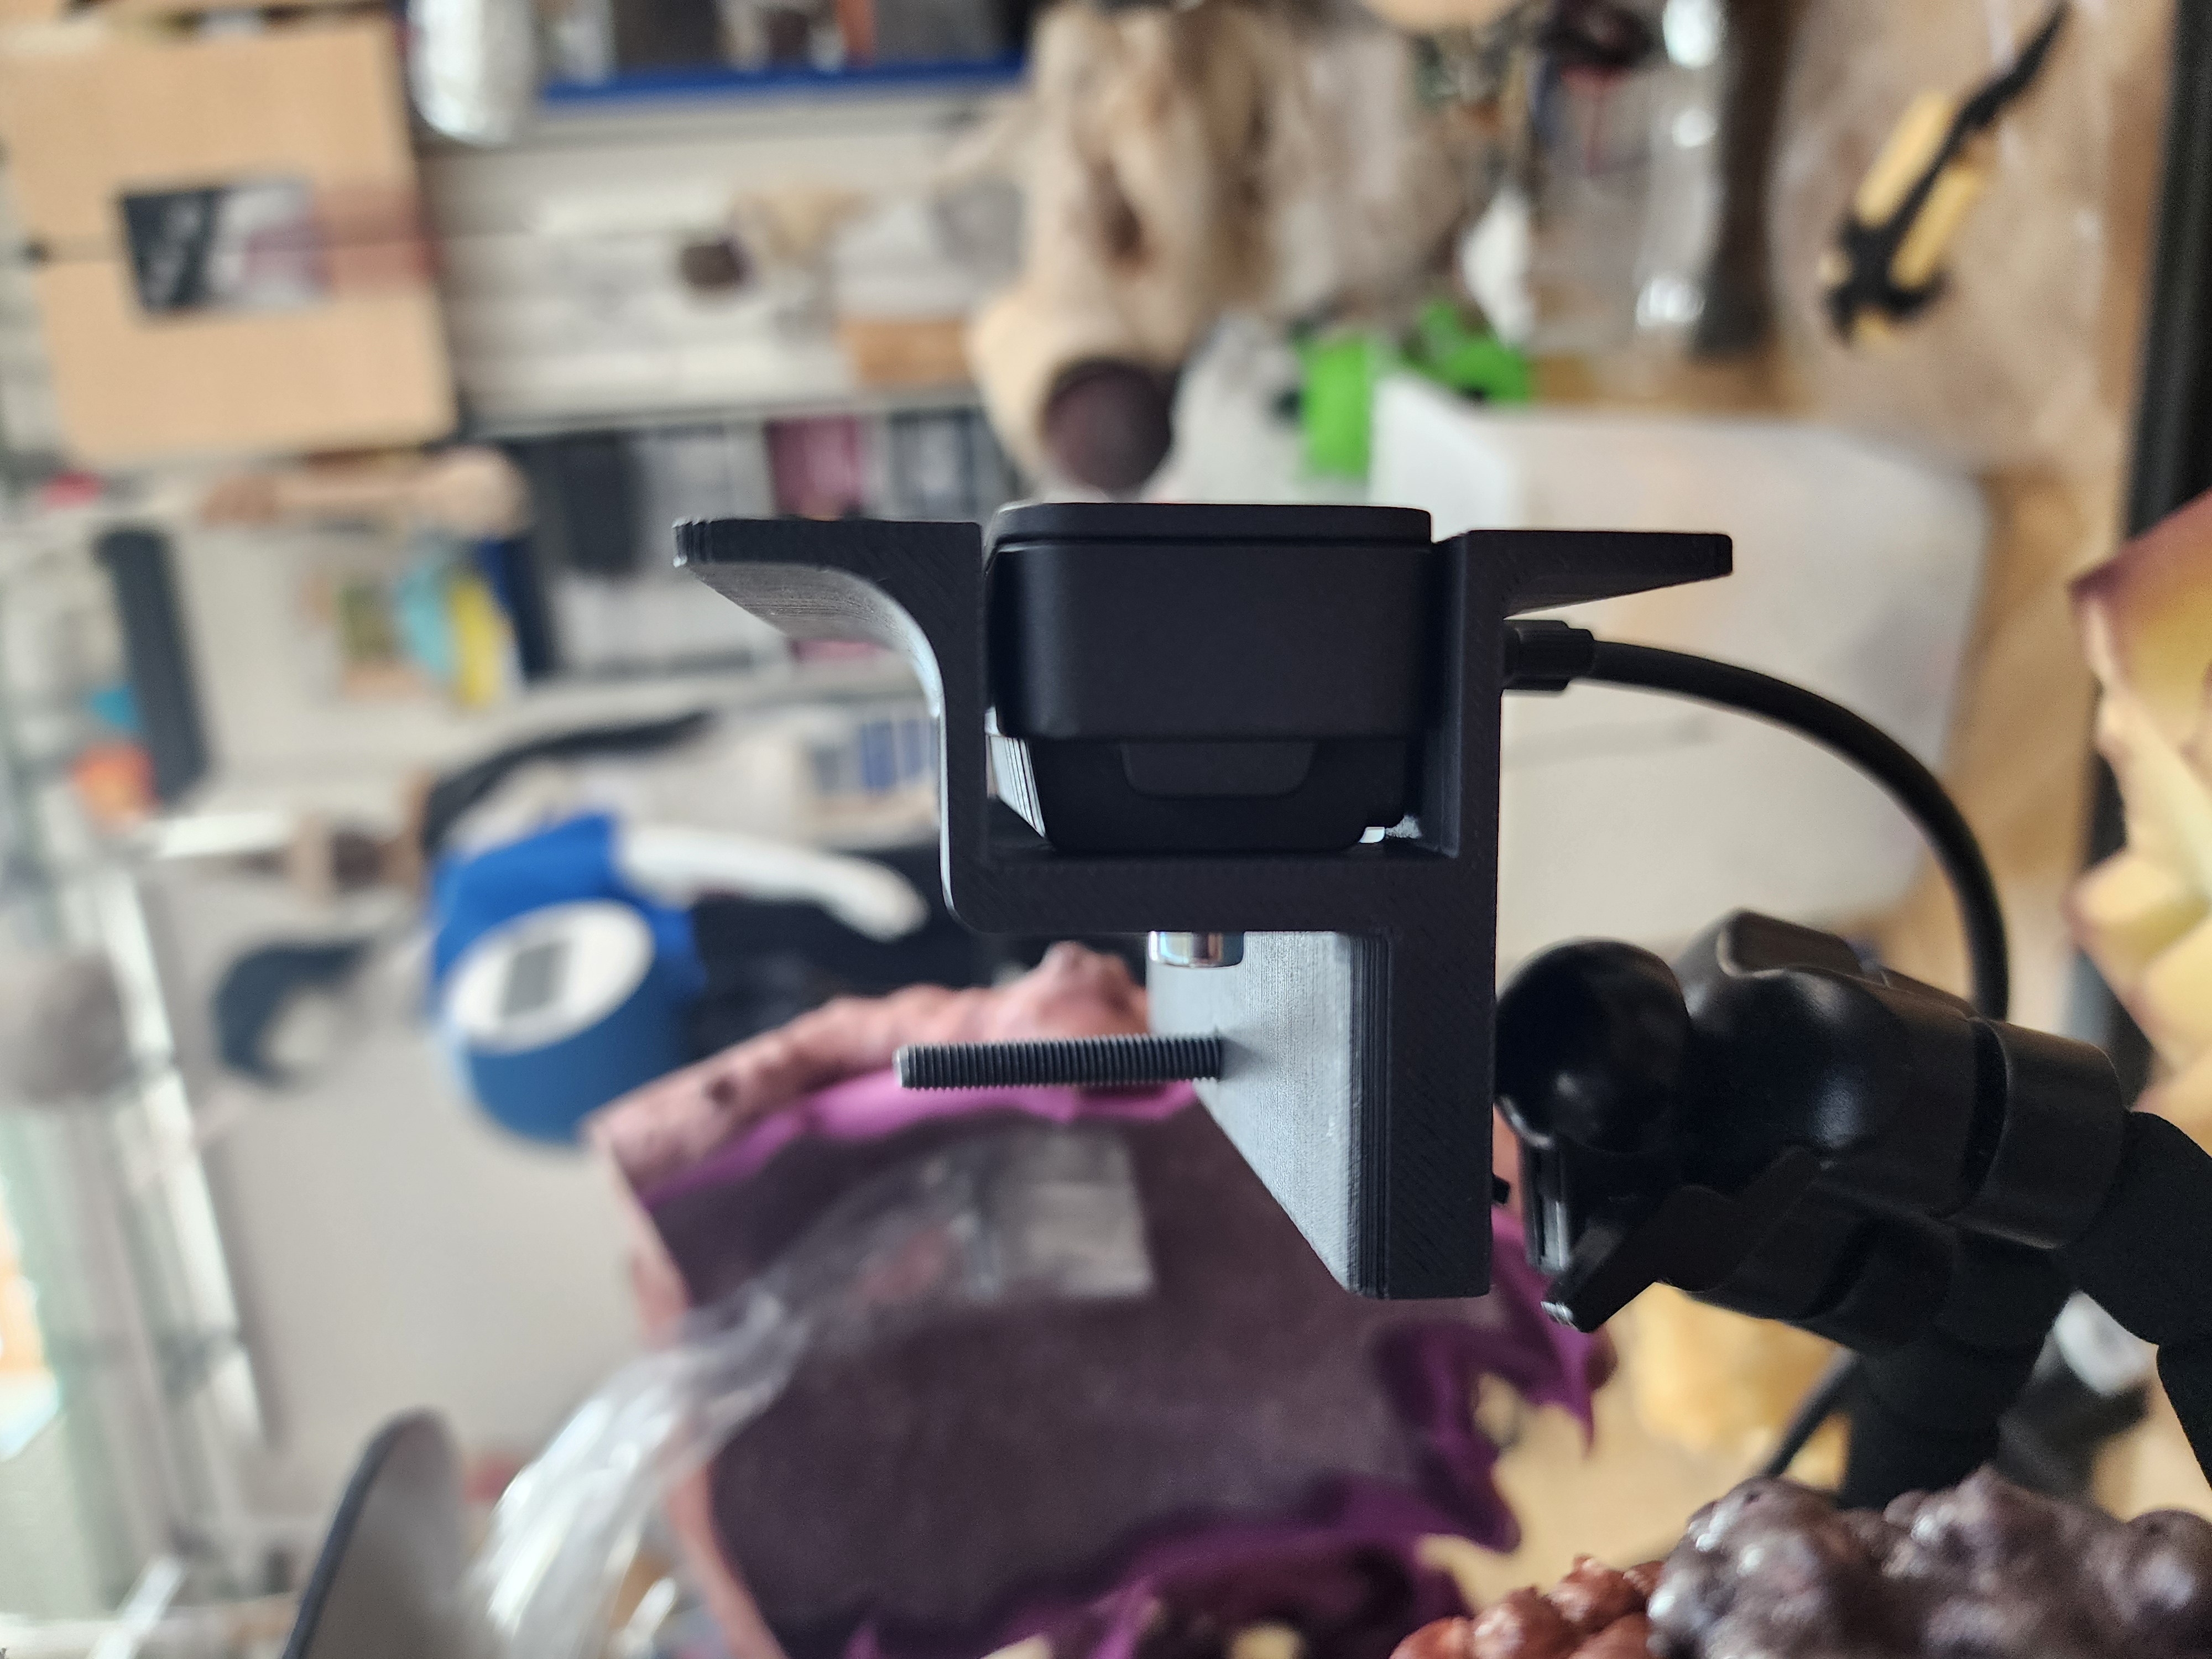
\includegraphics[width=\textwidth, angle=-90]{Images/CameraCasingNoMesh (4).jpg}
        \caption{Camera Casing without Mesh Covering (Side View)}
        \label{fig:camera_casing_no_mesh_side}
    \end{minipage}
    \hfill
    \begin{minipage}{0.45\textwidth}
        \centering
        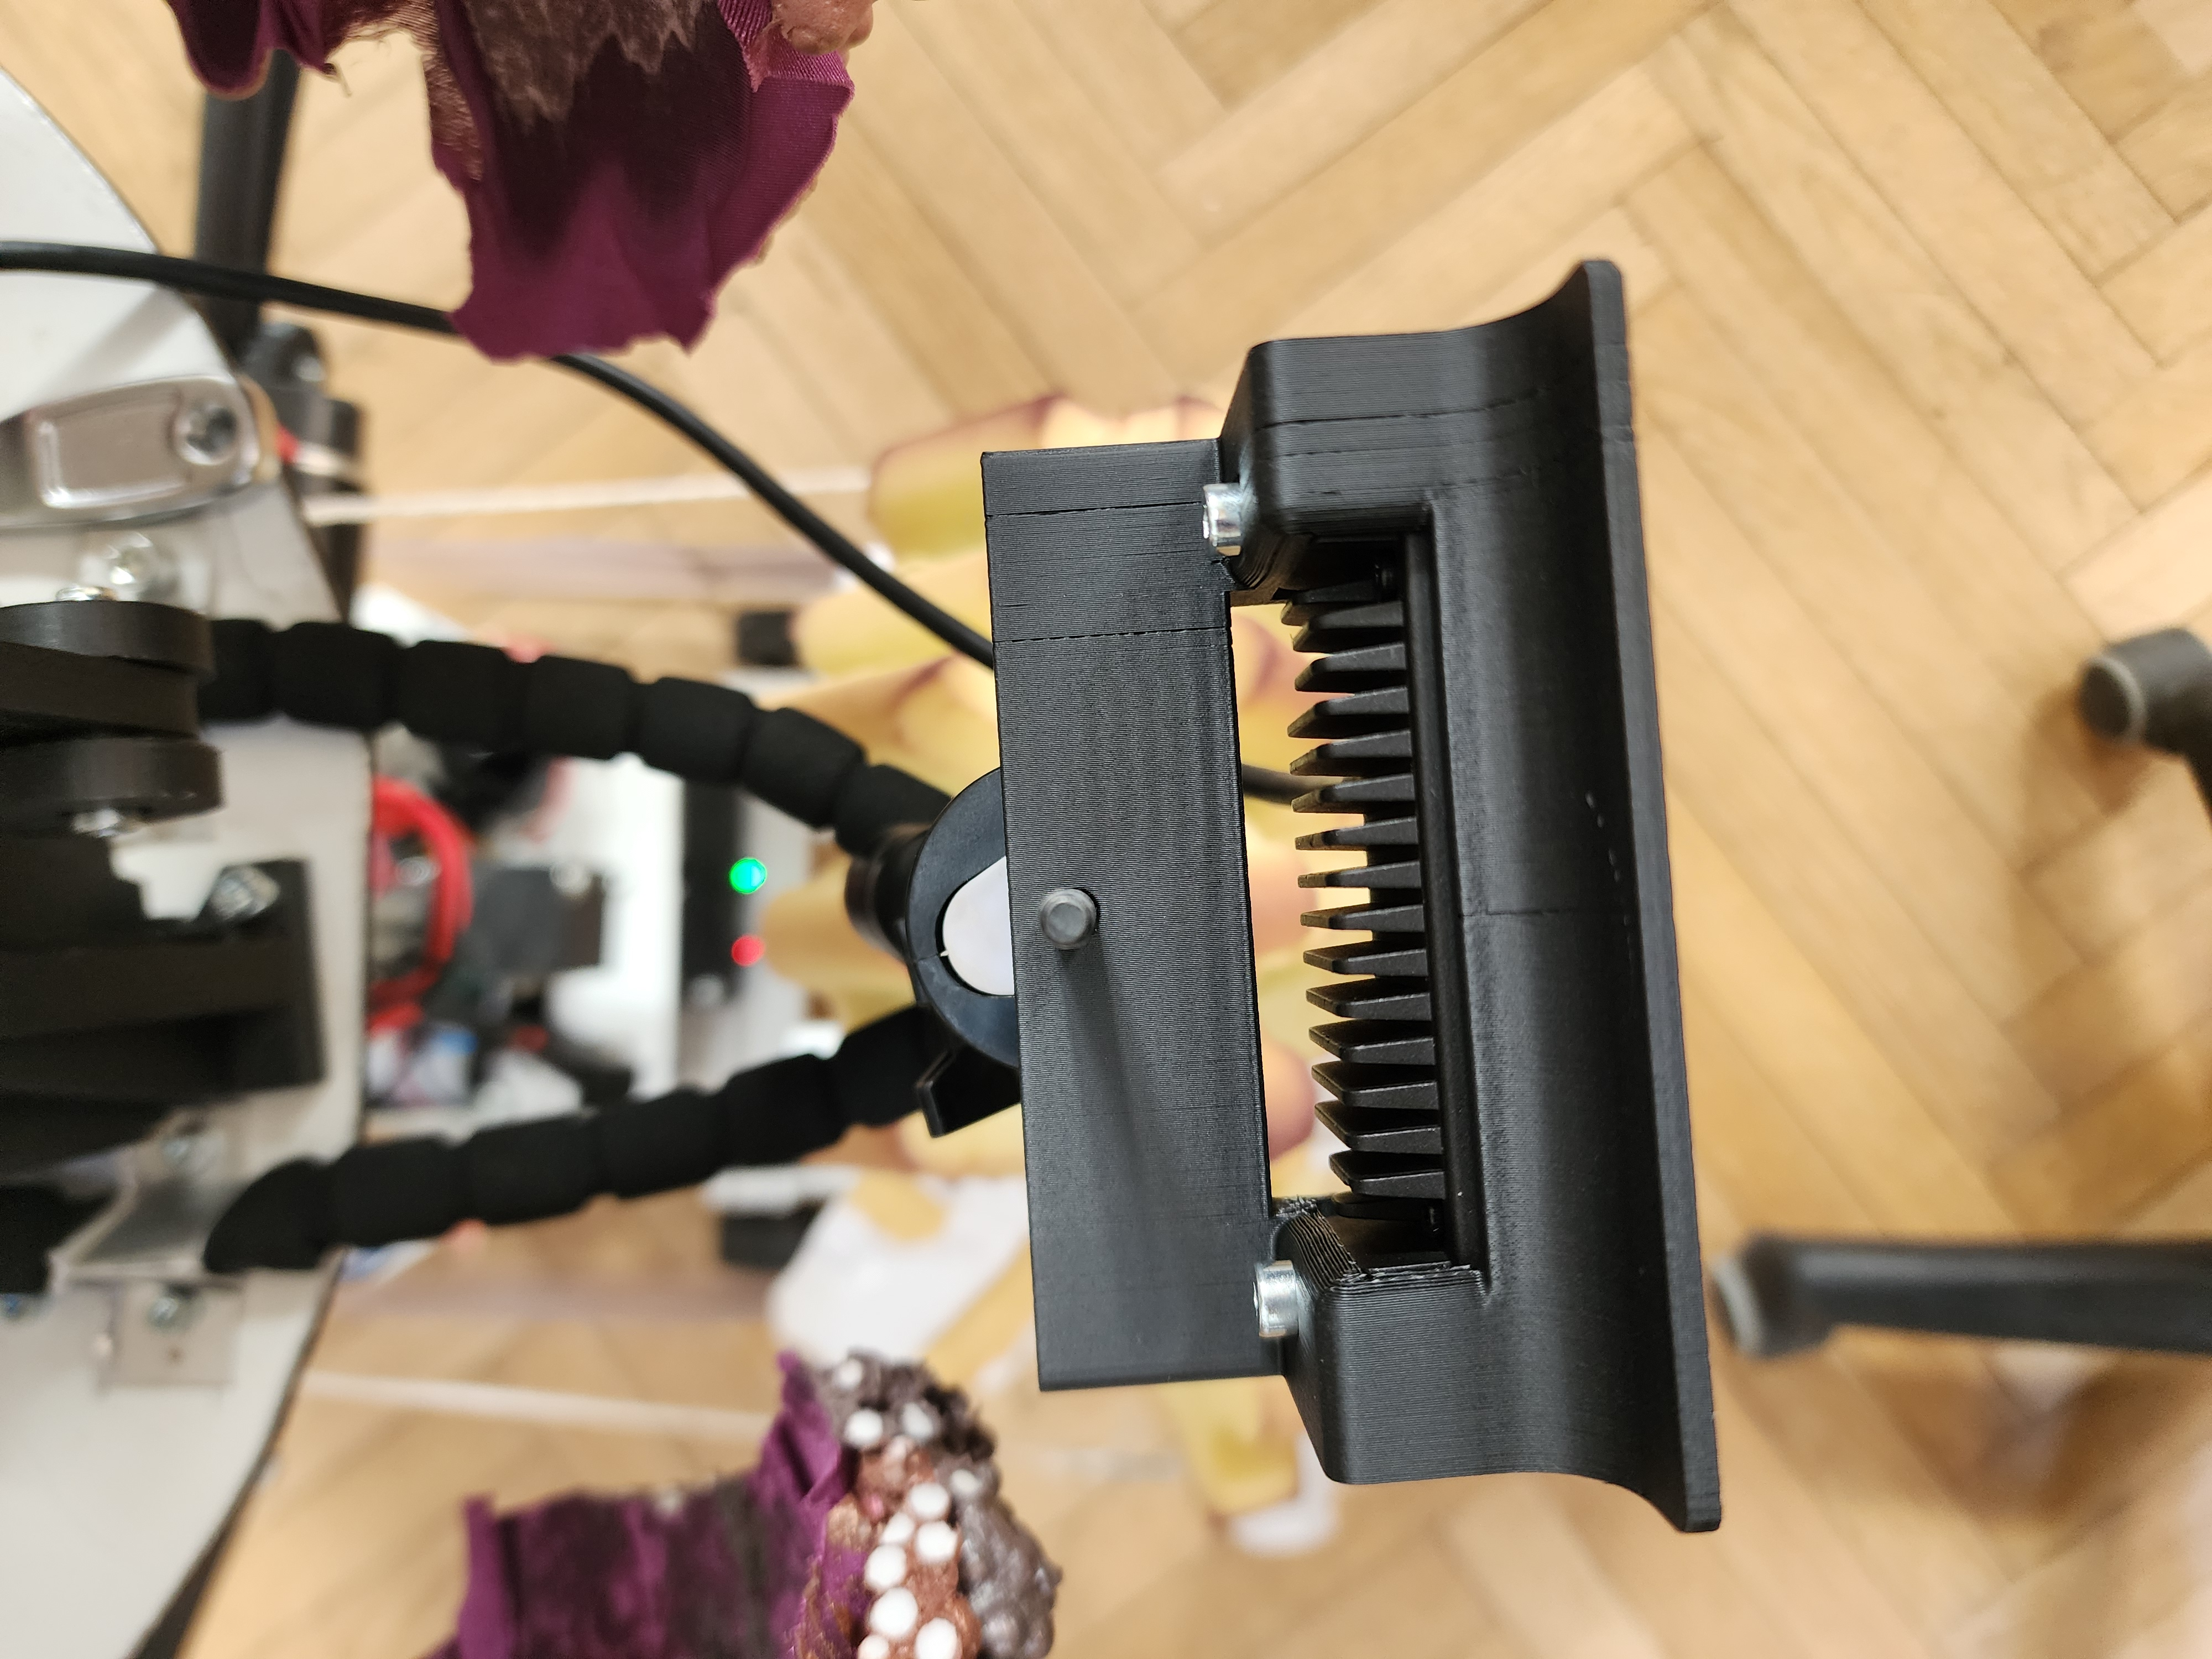
\includegraphics[width=\textwidth, angle=-90]{Images/CameraCasingNoMesh (3).jpg}
        \caption{Camera Casing without Mesh Covering (Top View)}
        \label{fig:camera_casing_no_mesh_top}
    \end{minipage}
\end{figure}

Field testing validates velcro system effectiveness during extended operational periods including various robot movements and interaction scenarios, ensuring consistent camera performance throughout typical social interaction scenarios while maintaining minimal image quality degradation.

% REORG_TAG: moved here from Audio System Integration
\subsection{Audio System Integration}

The audio system integration enables comprehensive bidirectional communication capabilities for VR integration and enhanced human-robot interaction, addressing the need for high-quality audio capture and dynamic sound generation that supports Tino's social presence and character expression. The system required careful hardware selection and sophisticated software implementation to achieve seamless integration with Tino's existing systems while maintaining acoustic performance within the constrained head environment.

\subsubsection{Hardware Implementation and Acoustic Design}

The audio hardware selection prioritized high-quality bidirectional communication capability while maintaining integration compatibility with Tino's system architecture and space constraints. The iTalk-01 omnidirectional microphone provides 360-degree audio capture capability suitable for social robot interaction scenarios where human positioning varies continuously, with microphone positioning optimization balancing audio quality against mechanical protection and aesthetic integration requirements through strategic fabric modifications.

The speaker system selection prioritized clear audio reproduction within the geometric and weight constraints of Tino's head assembly, with speaker placement within the servo head maximizing available space utilization while providing optimal acoustic coupling. Integration with existing head systems ensures speaker mounting does not interfere with Stewart platform operation, camera mounting, or other head-mounted systems.

\subsubsection{Speaker Mounting System Implementation}

The speaker system implementation prioritizes clear audio reproduction while addressing the practical requirements of maintenance access and acoustic optimization within Tino's constrained head geometry. The mounting solution utilizes industrial-grade velcro strips to secure speakers within the servo head structure, providing a robust yet flexible attachment system that enables quick realignment and maintenance without requiring complete head disassembly.

The velcro mounting system addresses several critical design challenges inherent in social robot audio integration. Primary considerations include vibration isolation to prevent mechanical noise transmission to the head structure, precise positioning control for optimal acoustic coupling, and maintenance accessibility for speaker replacement or cable management. The hook-and-loop fastener approach provides sufficient holding force to maintain speaker position during normal operation while enabling tool-free removal for system maintenance.

Speaker positioning optimization balances acoustic performance against space utilization within the head assembly. The mounting location maximizes available internal volume while ensuring speaker drivers remain clear of the Stewart platform mechanism, camera mounting hardware, and power distribution systems. Strategic positioning enables optimal sound projection through the fabric head covering while maintaining the structural integrity required for head articulation operations.

The velcro implementation includes strategic placement of adhesive-backed hook strips on the internal head structure and corresponding loop strips attached to custom speaker brackets. This configuration distributes mounting forces across multiple contact points, reducing stress concentration that could lead to attachment failure during extended operation. The system accommodates thermal expansion differences between speaker components and head structure materials while maintaining consistent acoustic coupling.

Installation procedures ensure proper alignment verification through acoustic testing and mechanical clearance validation. The removable nature of the velcro system enables rapid speaker replacement in field conditions, supporting efficient maintenance workflows that minimize robot downtime. Cable management integration ensures speaker wires remain secured and protected during head movement operations while maintaining accessibility for troubleshooting.

\begin{figure}[H]
    \centering
    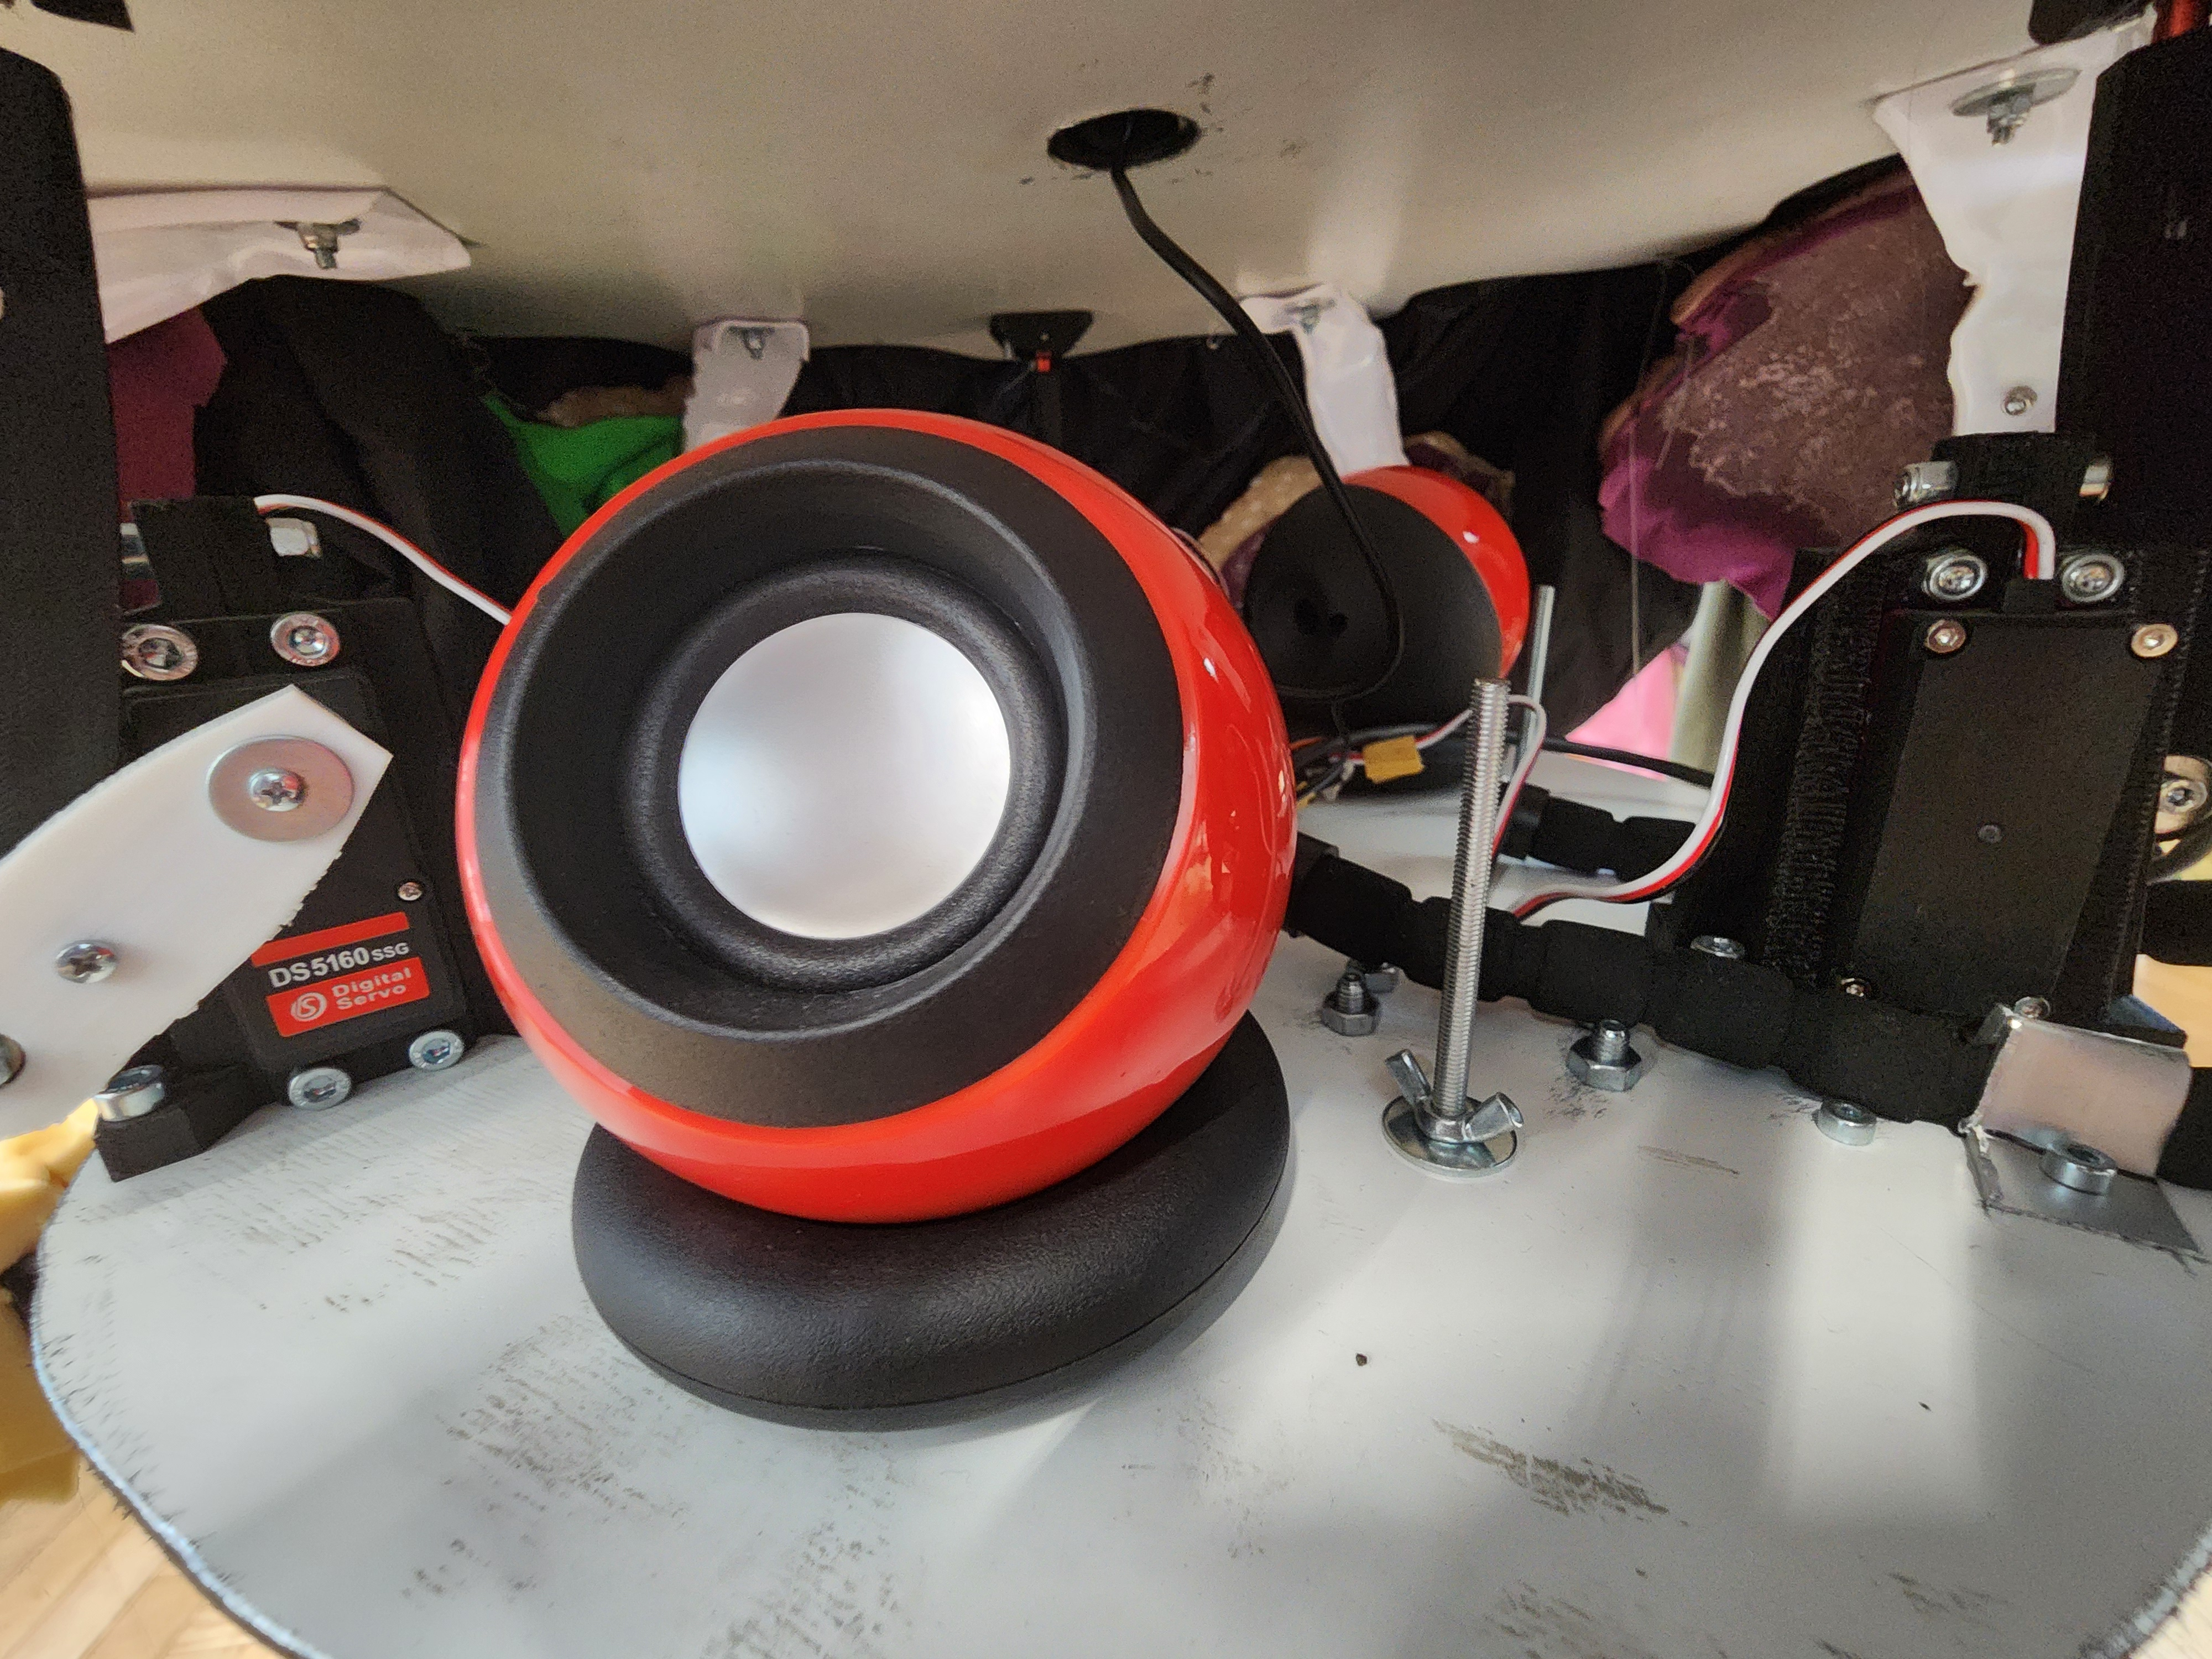
\includegraphics[height=6cm]{Images/SpeakerSetup (2).jpg}
    \caption{Speaker Mounted within Servo Head Structure}
    \label{fig:speaker_mount}
\end{figure}

\subsection{External Appearance Impact Assessment}

Throughout the comprehensive Tino V2 hardware implementation encompassing kinematic base redesign, power system overhaul, Stewart platform improvements, camera integration, and audio system enhancements, the robot's external aesthetic appearance has been deliberately preserved to maintain its distinctive character and proven social interaction capabilities.

The extensive internal modernization—from the fundamental shift to differential drive kinematics and enhanced power distribution to the complete redesign of head mechanisms and sensor integration—was strategically executed to operate within Tino's established external form factor. Each hardware upgrade was carefully engineered to enhance technical capabilities while preserving the approachable aesthetic that defines Tino's social robotics effectiveness. The fabric integration system, camera concealment mechanisms, and audio hardware placement all prioritize maintaining the robot's visual identity while enabling advanced functionality.

\begin{figure}[H]
    \centering
    \begin{minipage}{0.45\textwidth}
        \centering
        \includegraphics[width=\textwidth, angle=-90]{Images/TinoBefore.jpg}
        \caption{Tino Before V2 Implementation}
        \label{fig:tino_before_upgrade}
    \end{minipage}
    \hfill
    \begin{minipage}{0.45\textwidth}
        \centering
        \includegraphics[width=\textwidth, angle=-90]{Images/FinalTino.jpg}
        \caption{Tino After Complete V2 Upgrade}
        \label{fig:tino_after_upgrade}
    \end{minipage}
\end{figure}

The preservation of Tino's external design language validates the holistic engineering approach that achieved dramatic internal technological advancement while maintaining the established visual identity essential for consistent human-robot interaction research. This balance between comprehensive technical modernization and aesthetic continuity ensures that the V2 platform delivers enhanced capabilities without compromising the social robotics research foundation established by the original design, enabling seamless transition to the upgraded system while maintaining research validity and experimental continuity.

The comprehensive hardware implementation detailed throughout this section establishes the foundational platform that enables Tino V2's advanced capabilities. The kinematic base redesign provides the mobility precision required for sophisticated navigation algorithms, while the enhanced power distribution system supports the computational demands of modern perception and control systems. The redesigned Stewart platform head mechanism enables the fine-grained articulation necessary for natural social interaction, and the integrated camera system provides the visual input essential for advanced human-robot interaction. Most critically, the meticulously engineered audio hardware foundation—from microphone positioning for optimal capture to the velcro-mounted speaker system for maintenance accessibility—enables the sophisticated dynamic audio generation and VR integration capabilities that define Tino's enhanced social presence. This hardware foundation directly enables the advanced ROS2 software architecture, real-time VR integration, and intelligent audio generation algorithms detailed in the following chapter, where hardware capabilities transform into sophisticated robot behaviors that push the boundaries of social robotics.

